\RequirePackage[l2tabu,orthodox]{nag}

% TODO: decide if one-sided/two-sided
\documentclass[headsepline,footsepline,footinclude=false,fontsize=11pt,paper=a4,listof=totoc,bibliography=totoc,BCOR=12mm,DIV=12]{scrbook} % two-sided
% \documentclass[headsepline,footsepline,footinclude=false,oneside,fontsize=11pt,paper=a4,listof=totoc,bibliography=totoc]{scrbook} % one-sided
% \documentclass[headsepline,footsepline,footinclude=false,oneside,fontsize=11pt,paper=a4,listof=totoc,bibliography=totoc,DIV=12]{scrbook} 

\PassOptionsToPackage{table,svgnames,dvipsnames}{xcolor}

\usepackage[utf8]{inputenc}
\usepackage[T1]{fontenc}
\usepackage[sc]{mathpazo}
\usepackage[ngerman,english]{babel}
\usepackage[autostyle]{csquotes}
\usepackage[%
  backref=true,
  backend=biber,
  url=true,
  style=numeric,
  sorting=none,
  maxnames=4,
  minnames=3,
  maxbibnames=99,
  giveninits,
  uniquename=init]{biblatex}

\DefineBibliographyStrings{english}{%
  backrefpage = {page},% originally "cited on page"
  backrefpages = {pages},% originally "cited on pages"
}

\usepackage{graphicx}
\usepackage{scrhack} 
\usepackage{listings}
\usepackage{lstautogobble}
\usepackage{tikz}
\usepackage{pgfplots}
\usepackage{pgfplotstable}
\usepackage{booktabs} % for better looking table creations, but bad with vertical lines by design (package creator despises vertical lines)
\usepackage[final]{microtype}

\usepackage{caption}
\usepackage{subcaption}
\usepackage[font={small,it}, labelfont=bf]{caption}
\usepackage[hidelinks]{hyperref} 
% \usepackage{hyperref}
\hypersetup{
    colorlinks=true,
    linkcolor=black,
    citecolor=blue,
    filecolor=magenta,      
    urlcolor=cyan,
}

\usepackage{pdftexcmds} 
\usepackage{paralist} 
% \usepackage{subfig} 

\usepackage{siunitx}
\usepackage{multirow} 
\usepackage[normalem]{ulem}
\useunder{\uline}{\ul}{}
\usepackage{array} 
\usepackage{makecell}
\usepackage{pdfpages}
\usepackage{adjustbox}
\usepackage{tablefootnote}
\usepackage{threeparttable}

% % Figures .ps
% \usepackage{auto-pst-pdf}
% \usepackage{epsf} 
\usepackage{float}


\usepackage{amssymb}
\usepackage{pifont}
\newcommand{\cmark}{\ding{51}}
\newcommand{\xmark}{\ding{55}}


\usepackage[acronym,xindy,toc]{glossaries}
\makeglossaries
\loadglsentries{pages/glossary.tex} 


\bibliography{bibliography}

\setkomafont{disposition}{\normalfont\bfseries} 
\linespread{1.05} 
\setlength{\parskip}{0.75em}
% \setlength{\parskip}{0pt}
% \setlength{\parsep}{0pt}
% \setlength{\headsep}{0pt}
% \setlength{\topskip}{0pt}
% \setlength{\topmargin}{0pt}
% \setlength{\topsep}{0pt}
% \setlength{\partopsep}{0pt}

\BeforeTOCHead[toc]{{\cleardoublepage\pdfbookmark[0]{\contentsname}{toc}}}

% Define TUM corporate design colors
% Taken from http://portal.mytum.de/corporatedesign/index_print/vorlagen/index_farben
\definecolor{TUMBlue}{HTML}{0065BD}
\definecolor{TUMSecondaryBlue}{HTML}{005293}
\definecolor{TUMSecondaryBlue2}{HTML}{003359}
\definecolor{TUMBlack}{HTML}{000000}
\definecolor{TUMWhite}{HTML}{FFFFFF}
\definecolor{TUMDarkGray}{HTML}{333333}
\definecolor{TUMGray}{HTML}{808080}
\definecolor{TUMLightGray}{HTML}{CCCCC6}
\definecolor{TUMAccentGray}{HTML}{DAD7CB}
\definecolor{TUMAccentOrange}{HTML}{E37222}
\definecolor{TUMAccentGreen}{HTML}{A2AD00}
\definecolor{TUMAccentLightBlue}{HTML}{98C6EA}
\definecolor{TUMAccentBlue}{HTML}{64A0C8}

% Settings for pgfplots
\pgfplotsset{compat=newest}
\pgfplotsset{
  cycle list={TUMBlue\\TUMAccentOrange\\TUMAccentGreen\\TUMSecondaryBlue2\\TUMDarkGray\\},
}

% Settings for lstlistings
\definecolor{codegreen}{rgb}{0,0.6,0}
\definecolor{codegray}{rgb}{0.5,0.5,0.5}
\definecolor{codepurple}{rgb}{0.58,0,0.82}
\definecolor{backcolour}{rgb}{0.95,0.95,0.92}
 
\lstdefinestyle{mystyle}{
    backgroundcolor=\color{backcolour},   
    commentstyle=\color{codegreen},
    keywordstyle=\color{magenta},
    numberstyle=\tiny\color{codegray},
    stringstyle=\color{codepurple},
    basicstyle=\ttfamily\footnotesize,
    breakatwhitespace=false,         
    breaklines=true,                 
    captionpos=b,                    
    keepspaces=true,                 
    numbers=left,                    
    numbersep=5pt,                  
    showspaces=false,                
    showstringspaces=false,
    showtabs=false,                  
    tabsize=2
}

% Use this for basic highlighting
\lstset{%
  style=mystyle,
  basicstyle=\ttfamily,
  columns=fullflexible,
  autogobble,
  keywordstyle=\bfseries\color{TUMBlue},
  stringstyle=\color{TUMAccentGreen}
}

% Settings for search order of pictures
\graphicspath{
    {logos/}
    {figures/}
}

% Set up hyphenation rules for the language package when mistakes happen
\babelhyphenation[english]{
an-oth-er
ex-am-ple
}


\newcommand{\todo}[1]{{\bfseries{\scshape{\color{TUMAccentOrange}[(TODO: #1)]}}}} % for multiple paragraphs
\newcommand{\done}[1]{{\itshape{\scshape{\color{TUMAccentBlue}[(Done: #1)]}}}}

\newcommand{\tabitem}{~~\llap{\textbullet}~~}

\newcolumntype{P}[1]{>{\centering\arraybackslash}p{#1}} % for horizontal alignment with limited column width
\newcolumntype{M}[1]{>{\centering\arraybackslash}m{#1}} % for horizontal and vertical alignment with limited column width
\newcolumntype{L}[1]{>{\raggedright\arraybackslash}m{#1}} % for vertical alignment left with limited column width
\newcolumntype{R}[1]{>{\raggedleft\arraybackslash}m{#1}} % for vertical alignment right with limited column width

\newcommand*{\getUniversity}{Technische Universität München}
\newcommand*{\getFaculty}{Department of Informatics}
\newcommand*{\getTitle}{Distributed Deep Reinforcement Learning for Large Scale Robotic Simulations}
\newcommand*{\getTitleGer}{Titel der Abschlussarbeit}
\newcommand*{\getAuthor}{Amr Mohamed Kayid}
\newcommand*{\getDoctype}{Bachelor's Thesis in Informatics}
\newcommand*{\getAdvisor}{Benedikt Feldotto M.Sc.}
\newcommand*{\getSupervisor}{Prof. Dr.-Ing. Alois Christian Knoll}
\newcommand*{\getSubmissionDate}{August 8, 2019}
\newcommand*{\getSubmissionLocation}{Munich}

\begin{document}

\pagenumbering{alph}

\begin{titlepage}

  \oddsidemargin=\evensidemargin\relax
  \textwidth=\dimexpr\paperwidth-2\evensidemargin-2in\relax
  \hsize=\textwidth\relax

  \centering

  % \begin{center}
  %   \setlength{\tabcolsep}{0pt}
  %   \begin{tabular}{>{\raggedleft}m{2.5cm}>{\centering}m{\dimexpr\textwidth - 5cm\relax}>{\raggedright}m{2.5cm}}
  %   
\includegraphics[width=\linewidth]{logos/humanbrainproject.jpg}%
  %   &%
  %   \textbf{\large Human Brain Project} \\[5pt]%
  %   \textbf{\large Neurorobotics Platform}%
  %   &%
  %   
\includegraphics[width=\linewidth]{logos/nrp.png} %
  %   \end{tabular}
  % \end{center}

  \IfFileExists{logos/tum.png}{%
    
\includegraphics[height=20mm]{logos/tum.png}
  }{%
    \vspace*{20mm}
  }

  \vspace{5mm}
  {\huge\MakeUppercase{\getFaculty{}}}\\

  \vspace{5mm}
  {\large\MakeUppercase{\getUniversity{}}}\\

  \vspace{20mm}
  {\Large \getDoctype{}}

  \vspace{15mm}
  {\huge\bfseries \getTitle{}}

  \vspace{75mm}
  {\huge \getAuthor{}}

  \IfFileExists{logos/faculty.png}{%
    \vfill{}
    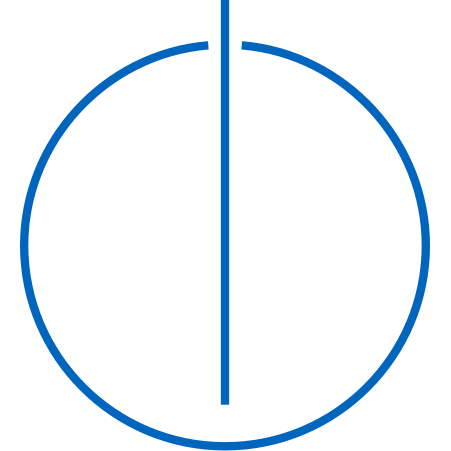
\includegraphics[height=20mm]{logos/faculty.png}
  }{}
  
\end{titlepage}


\frontmatter{}

\begin{titlepage}

  \centering

  \IfFileExists{logos/tum.png}{%
    
\includegraphics[height=20mm]{logos/tum.png}
  }{%
    \vspace*{20mm}
  }

  \vspace{5mm}
  {\huge\MakeUppercase{\getFaculty{}}}\\

  \vspace{5mm}
  {\large\MakeUppercase{\getUniversity{}}}\\

  \vspace{20mm}
  {\Large \getDoctype{}}

  \makeatletter
  \vspace{15mm}
  {\huge\bfseries \getTitle{}}


  \vspace{20mm}
  {\huge\bfseries \foreignlanguage{english}{\getTitle{}}}
  }
  \makeatother

  \vspace{15mm}
  \begin{tabular}{l l}
    Author:          & \getAuthor{} \\
    Supervisors:      & \getSupervisorOne{} \\ & \getSupervisorTwo{} \\
    Submission Date: & \getSubmissionDate{} \\
  \end{tabular}

  \IfFileExists{logos/faculty.png}{%
    \vfill{}
    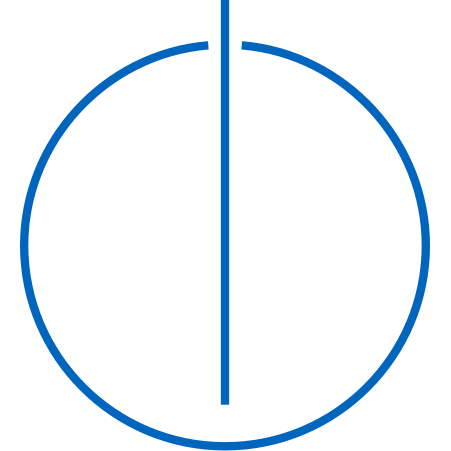
\includegraphics[height=20mm]{logos/faculty.png}
  }{}
  
\end{titlepage}

\cleardoublepage{}

\thispagestyle{empty}
\vspace*{0.8\textheight}
\noindent
{I confirm that this \MakeLowercase{\getDoctype{}} is my own work and I have documented all sources and material used.}

\vspace{15mm}
\noindent
\getSubmissionLocation{}, \getSubmissionDate{} \hspace{50mm} \getAuthor{}

\cleardoublepage{}

\addcontentsline{toc}{chapter}{Acknowledgments}
\thispagestyle{empty}

\vspace*{20mm}

\begin{center}
{\usekomafont{section} Acknowledgments}
\end{center}

\vspace{10mm}

% Acknowledgments
% Acknowledgments Acknowledgments Acknowledgments Acknowledgments Acknowledgments Acknowledgments Acknowledgments Acknowledgments Acknowledgments Acknowledgments Acknowledgments Acknowledgments Acknowledgments Acknowledgments Acknowledgments Acknowledgments Acknowledgments Acknowledgments Acknowledgments Acknowledgments Acknowledgments Acknowledgments Acknowledgments Acknowledgments Acknowledgments Acknowledgments Acknowledgments Acknowledgments Acknowledgments Acknowledgments Acknowledgments Acknowledgments Acknowledgments Acknowledgments Acknowledgments Acknowledgments Acknowledgments Acknowledgments Acknowledgments Acknowledgments Acknowledgments Acknowledgments Acknowledgments Acknowledgments Acknowledgments Acknowledgments Acknowledgments Acknowledgments Acknowledgments Acknowledgments Acknowledgments Acknowledgments Acknowledgments Acknowledgments Acknowledgments Acknowledgments Acknowledgments Acknowledgments Acknowledgments Acknowledgments Acknowledgments Acknowledgments Acknowledgments Acknowledgments Acknowledgments Acknowledgments Acknowledgments Acknowledgments Acknowledgments Acknowledgments Acknowledgments Acknowledgments Acknowledgments Acknowledgments Acknowledgments Acknowledgments Acknowledgments Acknowledgments Acknowledgments Acknowledgments Acknowledgments Acknowledgments Acknowledgments Acknowledgments Acknowledgments Acknowledgments Acknowledgments Acknowledgments Acknowledgments Acknowledgments 
% Acknowledgments Acknowledgments Acknowledgments Acknowledgments Acknowledgments Acknowledgments Acknowledgments Acknowledgments Acknowledgments Acknowledgments Acknowledgments Acknowledgments Acknowledgments Acknowledgments Acknowledgments Acknowledgments Acknowledgments Acknowledgments Acknowledgments Acknowledgments Acknowledgments Acknowledgments Acknowledgments Acknowledgments Acknowledgments Acknowledgments Acknowledgments Acknowledgments Acknowledgments Acknowledgments Acknowledgments Acknowledgments Acknowledgments Acknowledgments Acknowledgments Acknowledgments Acknowledgments Acknowledgments Acknowledgments Acknowledgments Acknowledgments Acknowledgments Acknowledgments Acknowledgments Acknowledgments Acknowledgments Acknowledgments Acknowledgments Acknowledgments Acknowledgments Acknowledgments Acknowledgments Acknowledgments Acknowledgments Acknowledgments Acknowledgments Acknowledgments Acknowledgments Acknowledgments Acknowledgments Acknowledgments Acknowledgments Acknowledgments Acknowledgments Acknowledgments Acknowledgments Acknowledgments Acknowledgments Acknowledgments Acknowledgments Acknowledgments Acknowledgments Acknowledgments Acknowledgments Acknowledgments Acknowledgments Acknowledgments Acknowledgments Acknowledgments Acknowledgments Acknowledgments Acknowledgments Acknowledgments Acknowledgments Acknowledgments Acknowledgments Acknowledgments Acknowledgments Acknowledgments Acknowledgments 
% Acknowledgments Acknowledgments Acknowledgments Acknowledgments Acknowledgments Acknowledgments Acknowledgments Acknowledgments Acknowledgments Acknowledgments Acknowledgments Acknowledgments Acknowledgments Acknowledgments Acknowledgments Acknowledgments Acknowledgments Acknowledgments Acknowledgments Acknowledgments Acknowledgments Acknowledgments Acknowledgments Acknowledgments Acknowledgments Acknowledgments Acknowledgments Acknowledgments Acknowledgments Acknowledgments Acknowledgments Acknowledgments Acknowledgments Acknowledgments Acknowledgments Acknowledgments Acknowledgments Acknowledgments Acknowledgments Acknowledgments Acknowledgments Acknowledgments Acknowledgments Acknowledgments Acknowledgments Acknowledgments Acknowledgments Acknowledgments Acknowledgments Acknowledgments Acknowledgments Acknowledgments Acknowledgments Acknowledgments Acknowledgments Acknowledgments Acknowledgments Acknowledgments Acknowledgments Acknowledgments Acknowledgments Acknowledgments Acknowledgments Acknowledgments Acknowledgments Acknowledgments Acknowledgments Acknowledgments Acknowledgments Acknowledgments Acknowledgments Acknowledgments Acknowledgments Acknowledgments Acknowledgments Acknowledgments Acknowledgments Acknowledgments Acknowledgments Acknowledgments Acknowledgments Acknowledgments Acknowledgments Acknowledgments Acknowledgments Acknowledgments Acknowledgments Acknowledgments Acknowledgments Acknowledgments 

% \cleardoublepage{}

\chapter{\abstractname}
Deep reinforcement learning enables algorithms to learn complex behavior, deal with continuous action spaces and find good strategies in environments with high dimensional state spaces. With deep reinforcement learning being an active area of research and many concurrent inventions, we decided to focus on a relatively simple robotic task to evaluate a set of ideas that might help to solve recent reinforcement learning problems. The focus on enabling distributed set up to execute and run an experiment with the least amount of time and benefit from the available computational power. Another focus is on the transferability between different physics engines, where we experiment on how to use a trained agent from one environment into another different environment with a different physics engine.

The purpose of this thesis is to unify the differences between different reinforcement learning environment by sharing a simple abstract API between the selected environments which can be extended to support more environment. With this, we focus only on setting and enabling distributed for training to reduce the time of the experiment. We select two of the state of the art reinforcement learning methods to train, evaluate and test the distributed and transferability. The goal of this strategy is to reduce training time and eventually help the algorithms to scale, collect experiences, and train the agents effectively. The concluding evaluation and results prove the general applicability of the described concepts by testing them using selected environments. These concepts might be reused for future experiments.

\microtypesetup{protrusion=false}
\tableofcontents{}
\microtypesetup{protrusion=true}


\mainmatter{}

% Chapters
% !TeX root = ../../main.tex
% Add the above to each chapter to make compiling the PDF easier in some editors.

\chapter{Setup and Implementation}\label{chapter:setup_and_implementation}

In this chapter, the full details of the setups will be introduced. First, the used software framework will be presented. Then, our environments architecture and integration with the framework will be explained. Then, a brief description for the agents and algorithms will be shown. Lastly, description for all the used environments in our experiments will be provided.

\section{Overview}

Our approach is to setup a distributed learning architecture to run multiple experiments between selected environment and compare the results between training in normal non-distributed and distributed modes. We selected relatively close environment to robotics simulation with continuous observation and action spaces. A new abstract classes is introduced to run with the selected framework and unify the differences between different environments and physics simulators. A selection of the state of the art algorithms is used to train our reinforcement learning agents and compare between the algorithm and the modes for each algorithm.

\section{Software}
\textbf{Ray Framework~\parencite{moritz2018ray}: } Ray is a fast and simple framework for building and running distributed applications. The same code can be run on a single machine to achieve efficient multiprocessing, and it can be used on a cluster for large computations. Ray provide high scalability and a unified API for a variety of applications which is very useful for our experiments. Ray executes tasks asynchronously to achieve parallelism enabling us to run multiple environments in the same experiment to benefit from collection more experiences and trajectories for the agent.

\textbf{OpenAI Gym~\parencite{brockman2016openai}: } openai gym is a toolkit for developing and comparing reinforcement learning algorithms. It supports teaching agents everything from walking to playing games like Pong or Pinball. It has an open source interface to reinforcement learning tasks which provides an easy-to-use suite of reinforcement learning tasks. 

The core gym interface is \textbf{Env}, which is the unified environment interface. 
The following are the methods for the abstracted gym Env:

\begin{itemize}
    \item \textit{\textbf{\colorbox{gray!20}{reset(self)}}}: Reset the environment's state. Returns observation.
    \item \textit{\textbf{\colorbox{gray!20}{step(self, action)}}}: Step the environment by one time-step. Returns observation, reward, done, info.
    \item \textit{\textbf{\colorbox{gray!20}{render(self, mode='human')}}}: Render one frame of the environment. The default mode will do something human friendly, such as pop up a window.
\end{itemize}

\textbf{Unity MLAgents~\parencite{juliani2018unity}: } unity mlagents toolkit is an open-source Unity plugin that enables games and simulations to serve as environments for training intelligent agents. It has more realistic and complex simulation environments. It provides the ability to flexibly configure
the simulation. By taking advantage of Unity as a simulation platform, the toolkit enables the development of learning environments which are rich in sensory and physical complexity, provide compelling cognitive challenges, and support dynamic multi-agent interaction. Agents can be trained using reinforcement learning, imitation learning, neuroevolution, or other machine learning methods through a simple-to-use Python API. They provide implementations of state-of-the-art algorithms to enable game developers and hobbyists to easily train intelligent agents for 2D, 3D and VR/AR games. We are using this to test running multiple agents in the same environment and compare the effect with one agent only. Also, to experiment the transferability between different physics simulators.

\section{Architecture}

At a high level, ray provides an \textbf{\colorbox{gray!20}{Trainer}} class which holds a policy for environment interaction. Through the trainer interface~\ref{fig:ray_trainer}, the policy can be trained, check-pointed, or an action computed. In multi-agent training, the trainer manages the querying and optimization of multiple policies at once. It provides custom resources configurations~\ref{fig:ray_config}, which can control the degree of parallelism used by setting the \colorbox{gray!20}{\texttt{num\_workers}} hyper-parameter for most algorithms. The number of GPUs the driver should use can be set via the \colorbox{gray!20}{\texttt{num\_gpus}} option. Similarly, the resource allocation to workers can be controlled via \colorbox{gray!20}{\texttt{num\_cpus\_per\_worker}}, \colorbox{gray!20}{\texttt{num\_gpus\_per\_worker}}, and \colorbox{gray!20}{\texttt{custom\_resources\_per\_worker}}. The number of GPUs can be a fractional quantity to allocate only a fraction of a GPU. For example, with DQN you can pack five trainers onto one GPU by setting \colorbox{gray!20}{\texttt{num\_gpus}: 0.2}.

\begin{figure}[H]
	\centering
	\begin{subfigure}[b]{0.4\textwidth}
		\centering
		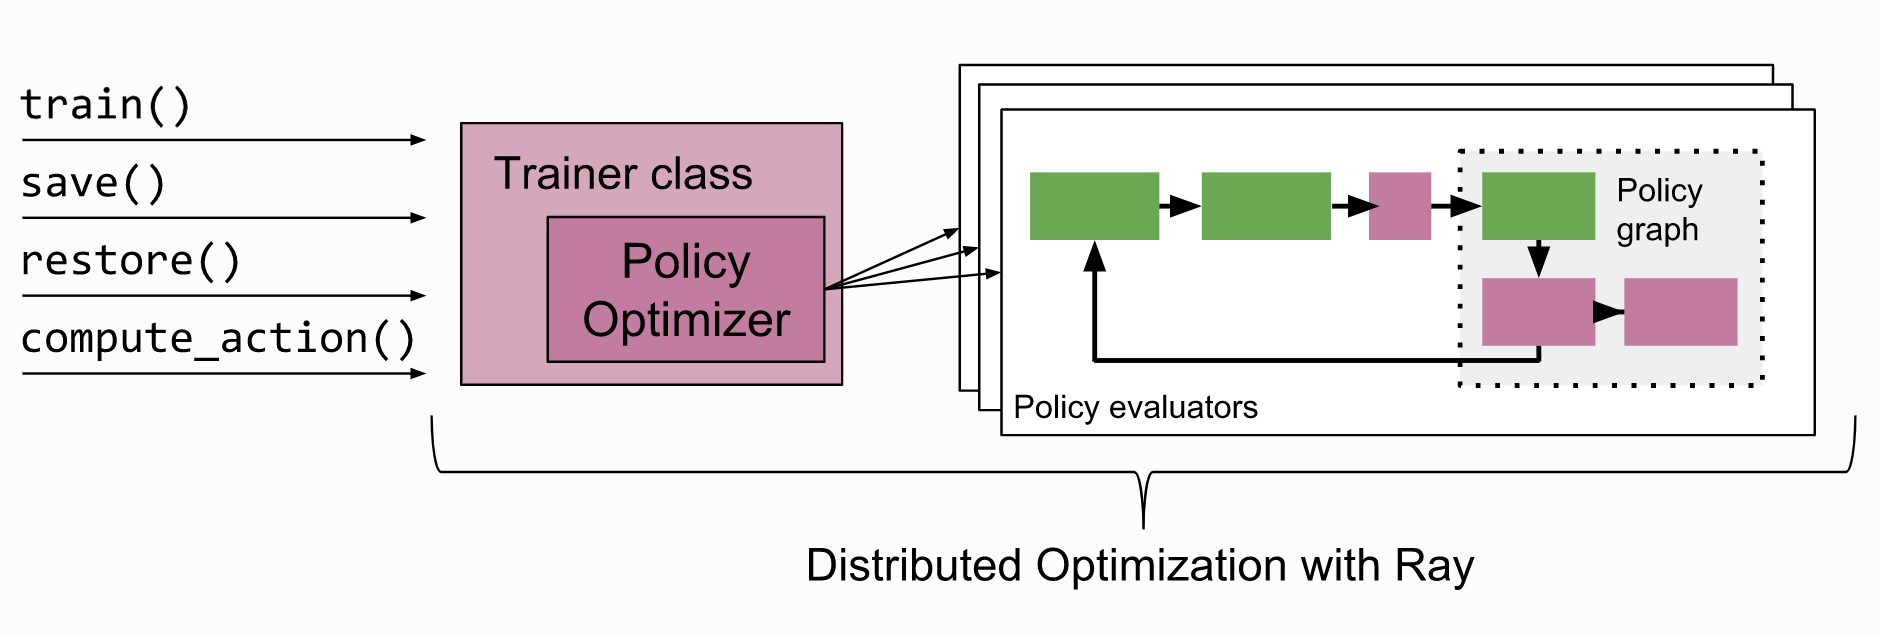
\includegraphics[width=\textwidth]{figures/architecture/ray_trainer.png}
		\caption{Ray Training Process}
		\label{fig:ray_trainer}
    \end{subfigure}
    \hfill
	\begin{subfigure}[b]{0.4\textwidth}
		\centering
		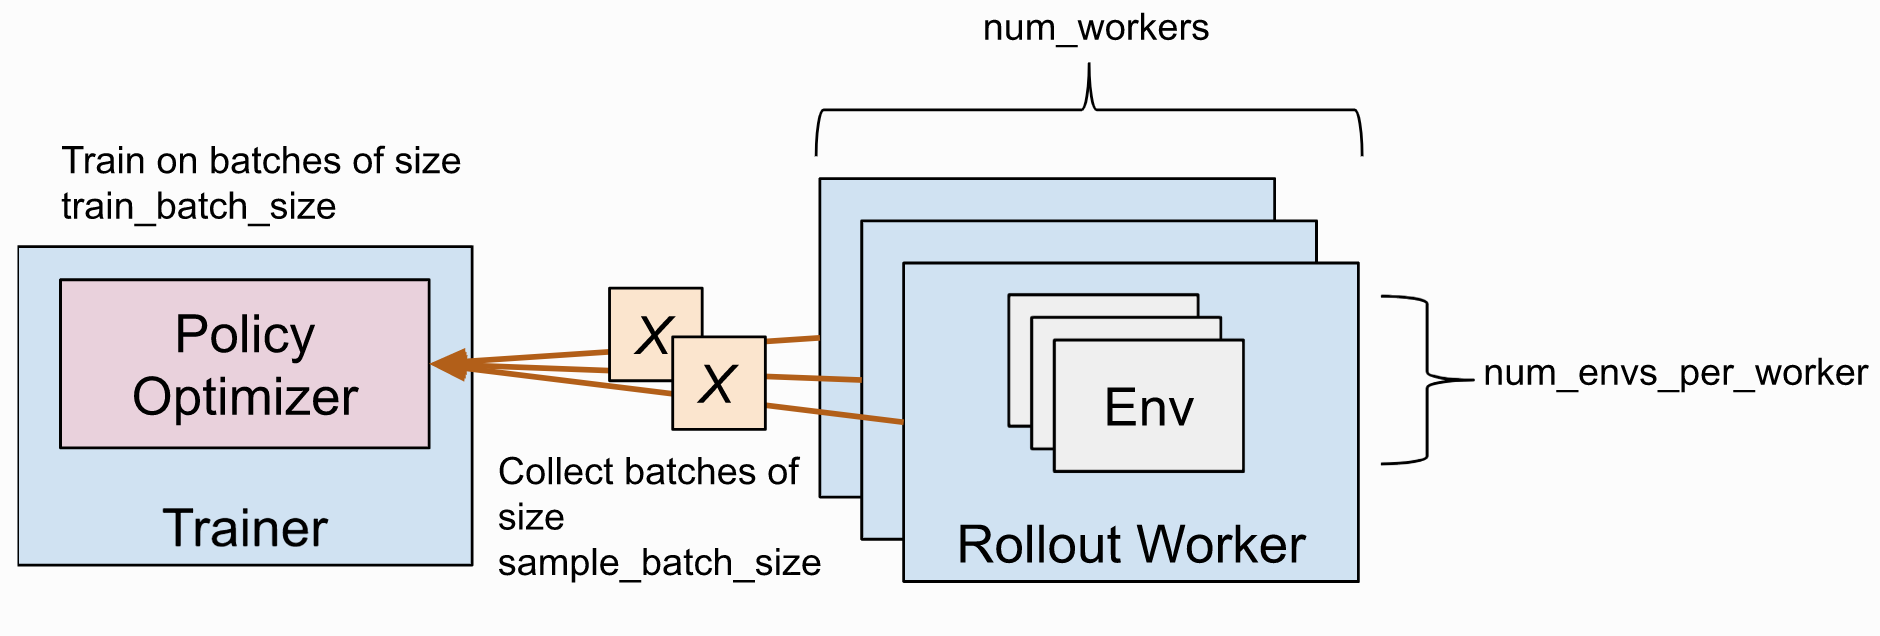
\includegraphics[width=\textwidth]{figures/architecture/ray_config.png}
        \caption{Ray Configurable resources}
		\label{fig:ray_config}
	\end{subfigure}
	\hfill
	   \caption{General Overview of Ray framework~\parencite{moritz2018ray}}
	   \label{fig:ray}
\end{figure}

Since ray support only OpenAI Gym environments along with their provided multi-agent and also batched environments, we had to implement our custom environment to unify between unity mlagents and openai gym environments. Also, we implemented our custom Multi-Agent environments for both used environments as shown in the following figure~\ref{fig:ray_envs}.

\begin{figure}[H]
	\centering
		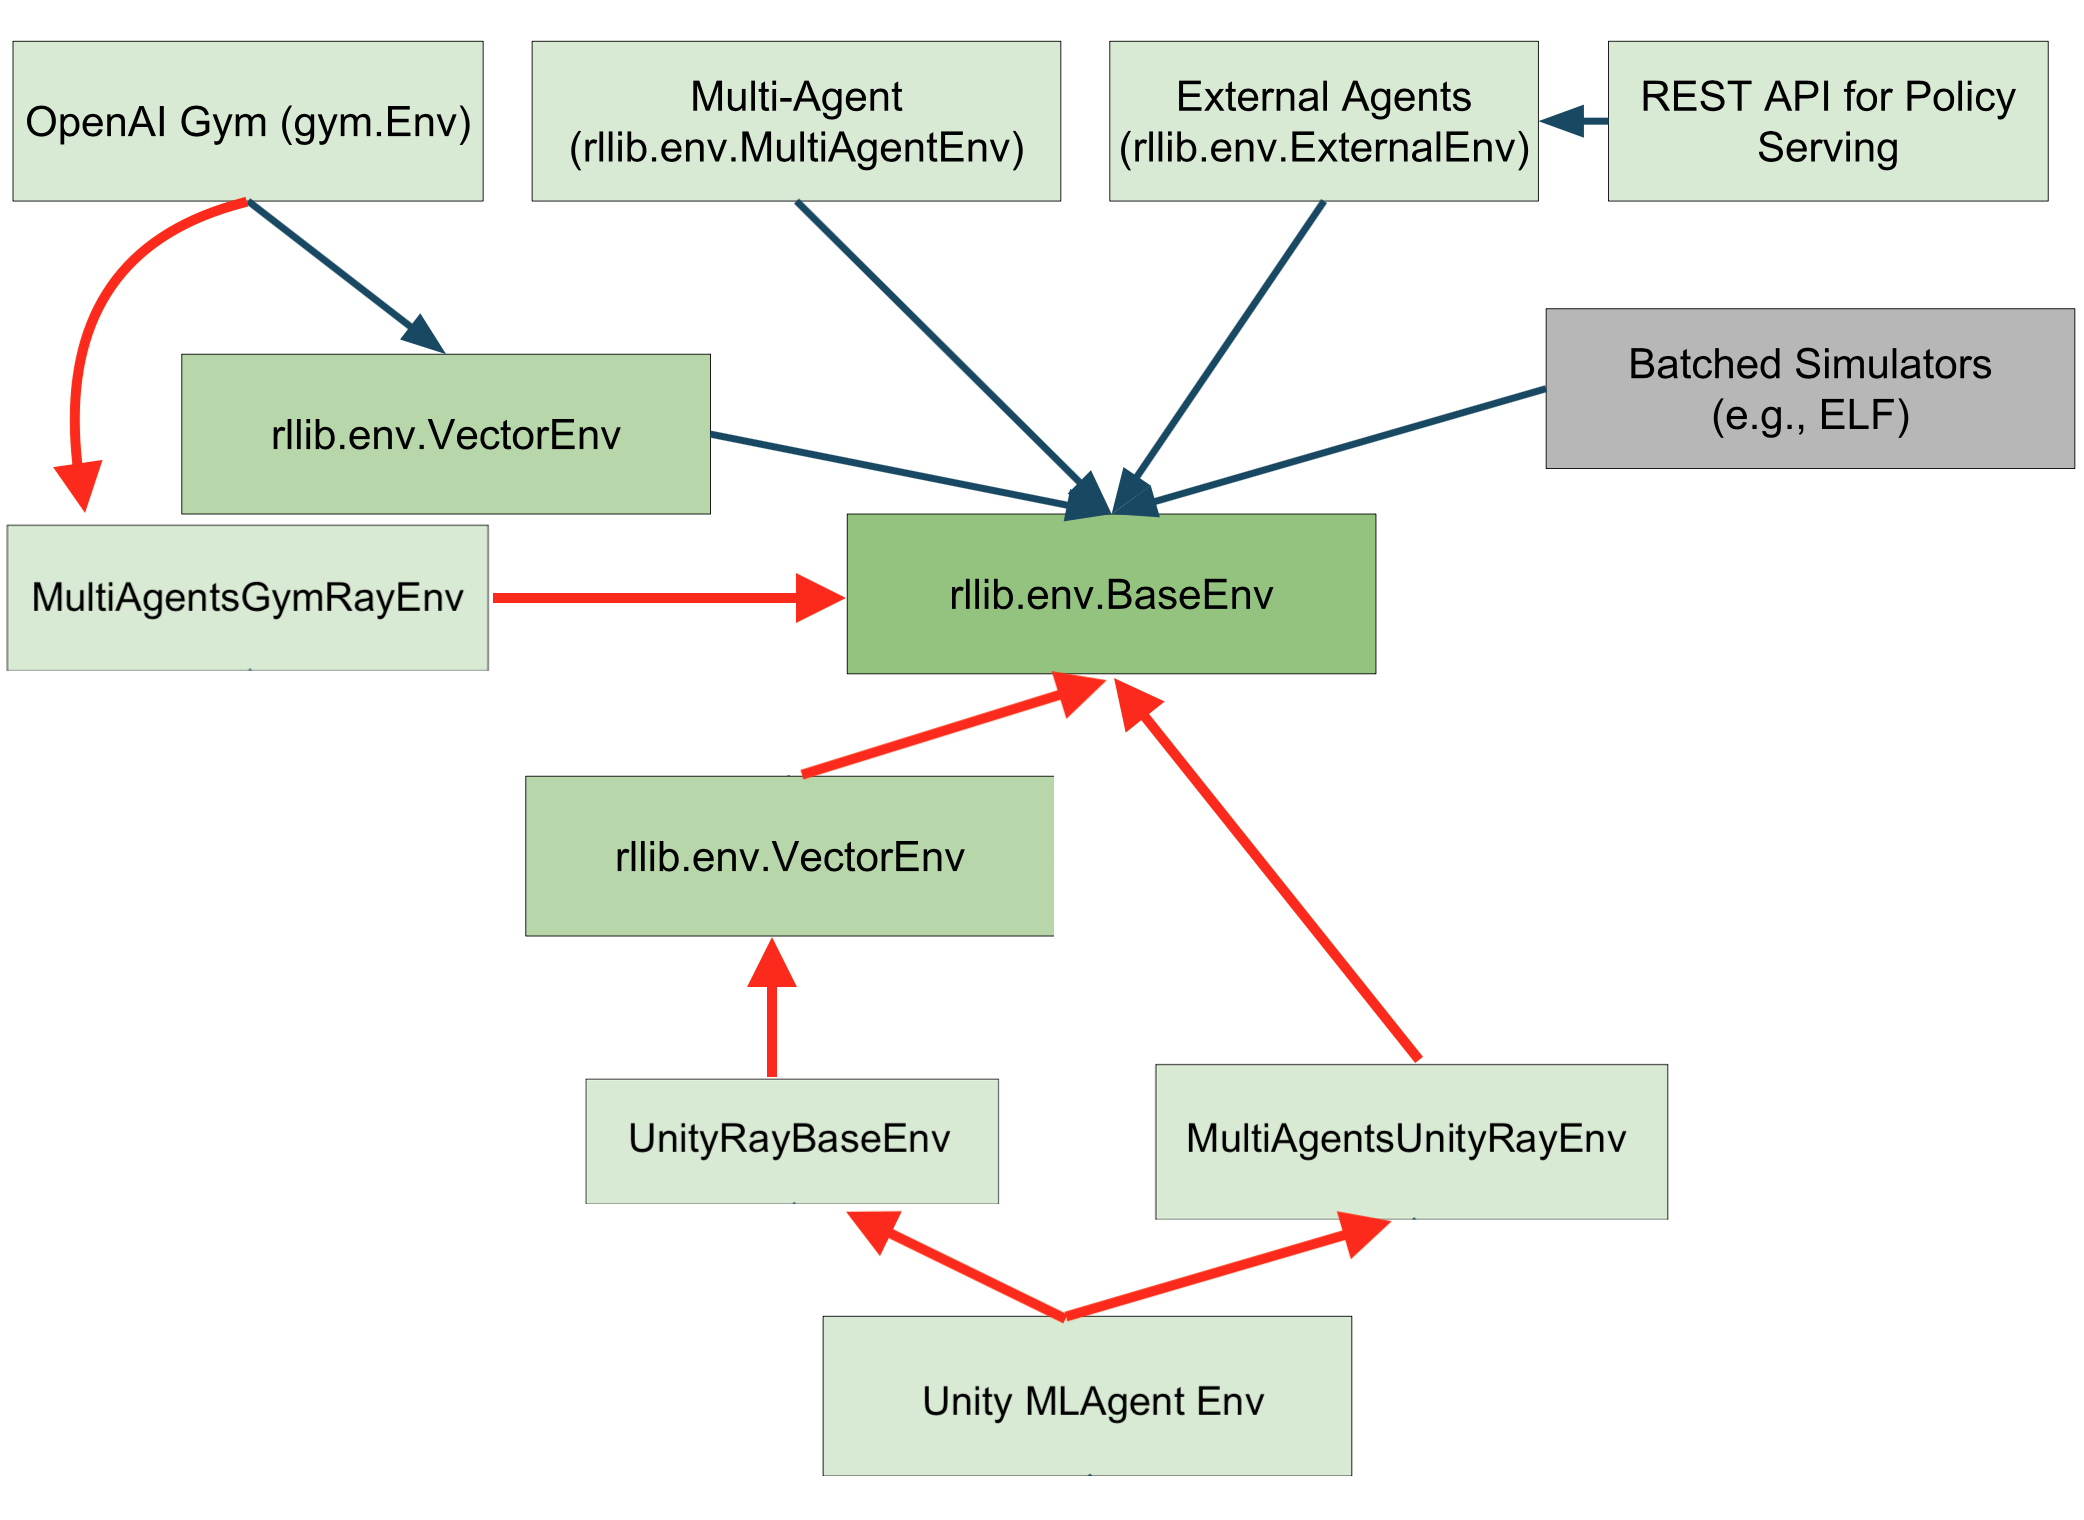
\includegraphics[width=\linewidth]{figures/architecture/ray_envs.png}
		\caption{Our Custom Environments}
		\label{fig:ray_envs}
\end{figure}

\clearpage

Custom environments implementations and methods are described below:

\textbf{UnityRayEnv}:\\
our base unity environment maps the observations and actions from unity mlagents toolkit to be compatible with Ray BaseEnv. Since unity mlagents deals with brains that control the agents and the environments we had to convert it to the required \colorbox{gray!20}{\texttt{observation\_space}} and \colorbox{gray!20}{\texttt{action\_space}} for ray env with the following methods:
\begin{itemize}
    \item \textit{\textbf{\colorbox{gray!20}{\texttt{\_\_init\_\_(self)}}}}: Create the unity environment from the unity build env, convert the observation and action spaces to be ray-compatible.
    \item \textit{\textbf{\colorbox{gray!20}{reset(self)}}}: Reset the environment's state. Returns observation.
    \item \textit{\textbf{\colorbox{gray!20}{step(self, action)}}}: Step the environment by one time-step. Returns observation, reward, done, info.
\end{itemize}

\textbf{MultiAgentsUnityRayEnv}:\\
this class inherit from both \colorbox{gray!20}{\textbf{UnityRayEnv}} and \colorbox{gray!20}{\textbf{MultiAgentEnv}}~\ref{fig:ray_multiagentenv}. The difference from the base environment is in both methods \textit{\textbf{\colorbox{gray!20}{reset(self)}}} and \textit{\textbf{\colorbox{gray!20}{step(self, \texttt{actions\_dict})}}}, where the reset function reset all the observations for each agent that exist in the environment and step function take a dictionary of actions corresponding for each action of a single agent. The same applies to \textbf{MultiAgentsGymRayEnv}.

\begin{figure}[H]
	\centering
		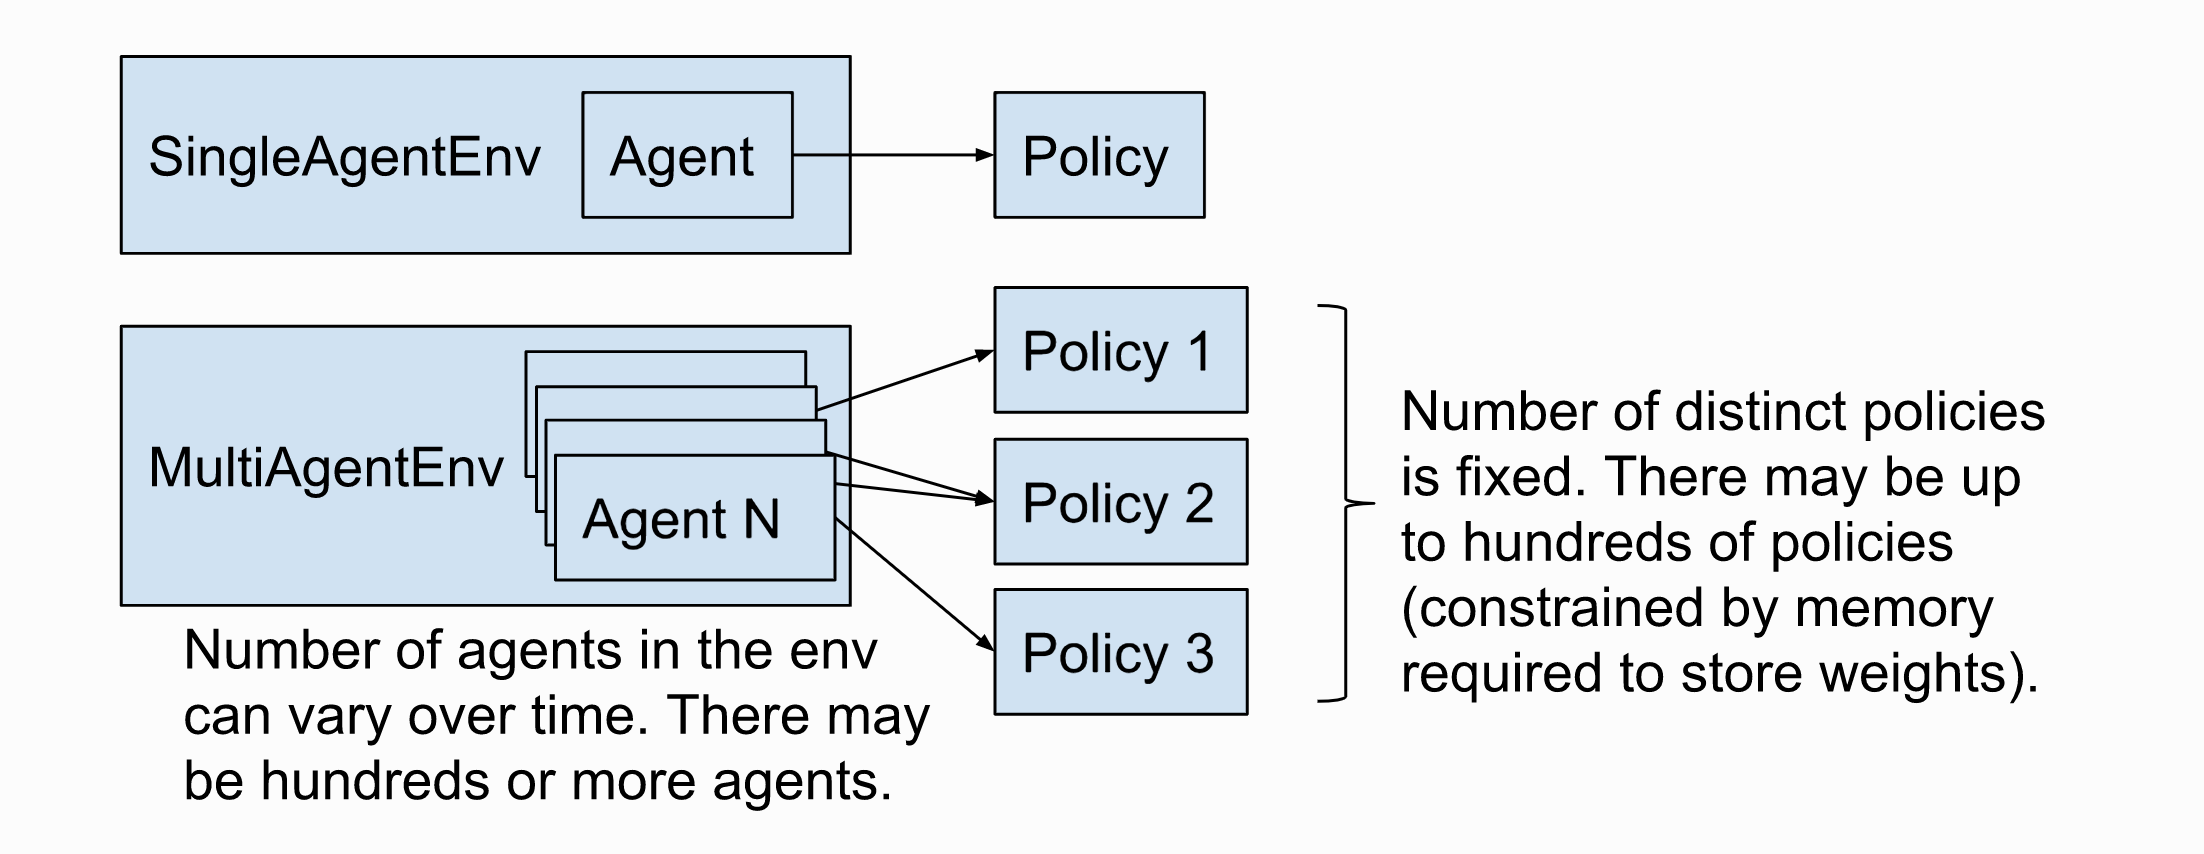
\includegraphics[width=\linewidth]{figures/architecture/ray_multiagentenv.png}
		\caption{Ray MultiAgentEnv}
		\label{fig:ray_multiagentenv}
\end{figure}

\section{Agents and Algorithms}

\begin{itemize}
    \item \textbf{Proximal Policy Optimization (PPO)}: PPO’s clipped objective supports multiple SGD passes over the same batch of experiences. RLlib’s multi-GPU optimizer pins that data in GPU memory to avoid unnecessary transfers from host memory, substantially improving performance over a naive implementation. RLlib’s PPO scales out using multiple workers for experience collection, and also with multiple GPUs for SGD.

    \item \textbf{Distributed Prioritized Experience Replay (Ape-X)}: Ape-X variations of DQN, DDPG, use a single GPU learner and many CPU workers for experience collection. Experience collection can scale to hundreds of CPU workers due to the distributed prioritization of experience prior to storage in replay buffers.

    \item \textbf{Importance Weighted Actor-Learner Architecture (IMPALA)}: In IMPALA, a central learner runs SGD in a tight loop while asynchronously pulling sample batches from many actor processes. RLlib’s IMPALA implementation uses DeepMind’s reference V-trace code. Note that we do not provide a deep residual network out of the box, but one can be plugged in as a custom model. Multiple learner GPUs and experience replay are also supported.
\end{itemize}

\section{Environments and Tasks Description}
Our task is robotic related task, where we have a robotic arm consist of two linked joints \textit{(agent)} and moving sphere \textit{(target)}. The robotic arm and the goal differ according to the environment used. We have a one experiment where is the agent movement is in 2D and the goal of the agent it to reach the target as fast as possible to maximize the given cumulative reward. In the second experiment, the agent can move in 3D and the goal is to keep track of the moving target and move with it along the 3D space.

Following is detailed description for all the environment used in our experiments.

\textbf{OpenAI: Reacher Environment}

Our first and baseline environment is \textit{Reacher Environment}~\ref{fig:openai_reacher}: A robotic arm consist of two linked joints places in a squared arena surrounding it along with a moving sphere (target). The goal of the robotics arm it to reach target sphere and maintain following the point until the end of the episode. 

\begin{figure}[H]
    \begin{center}
            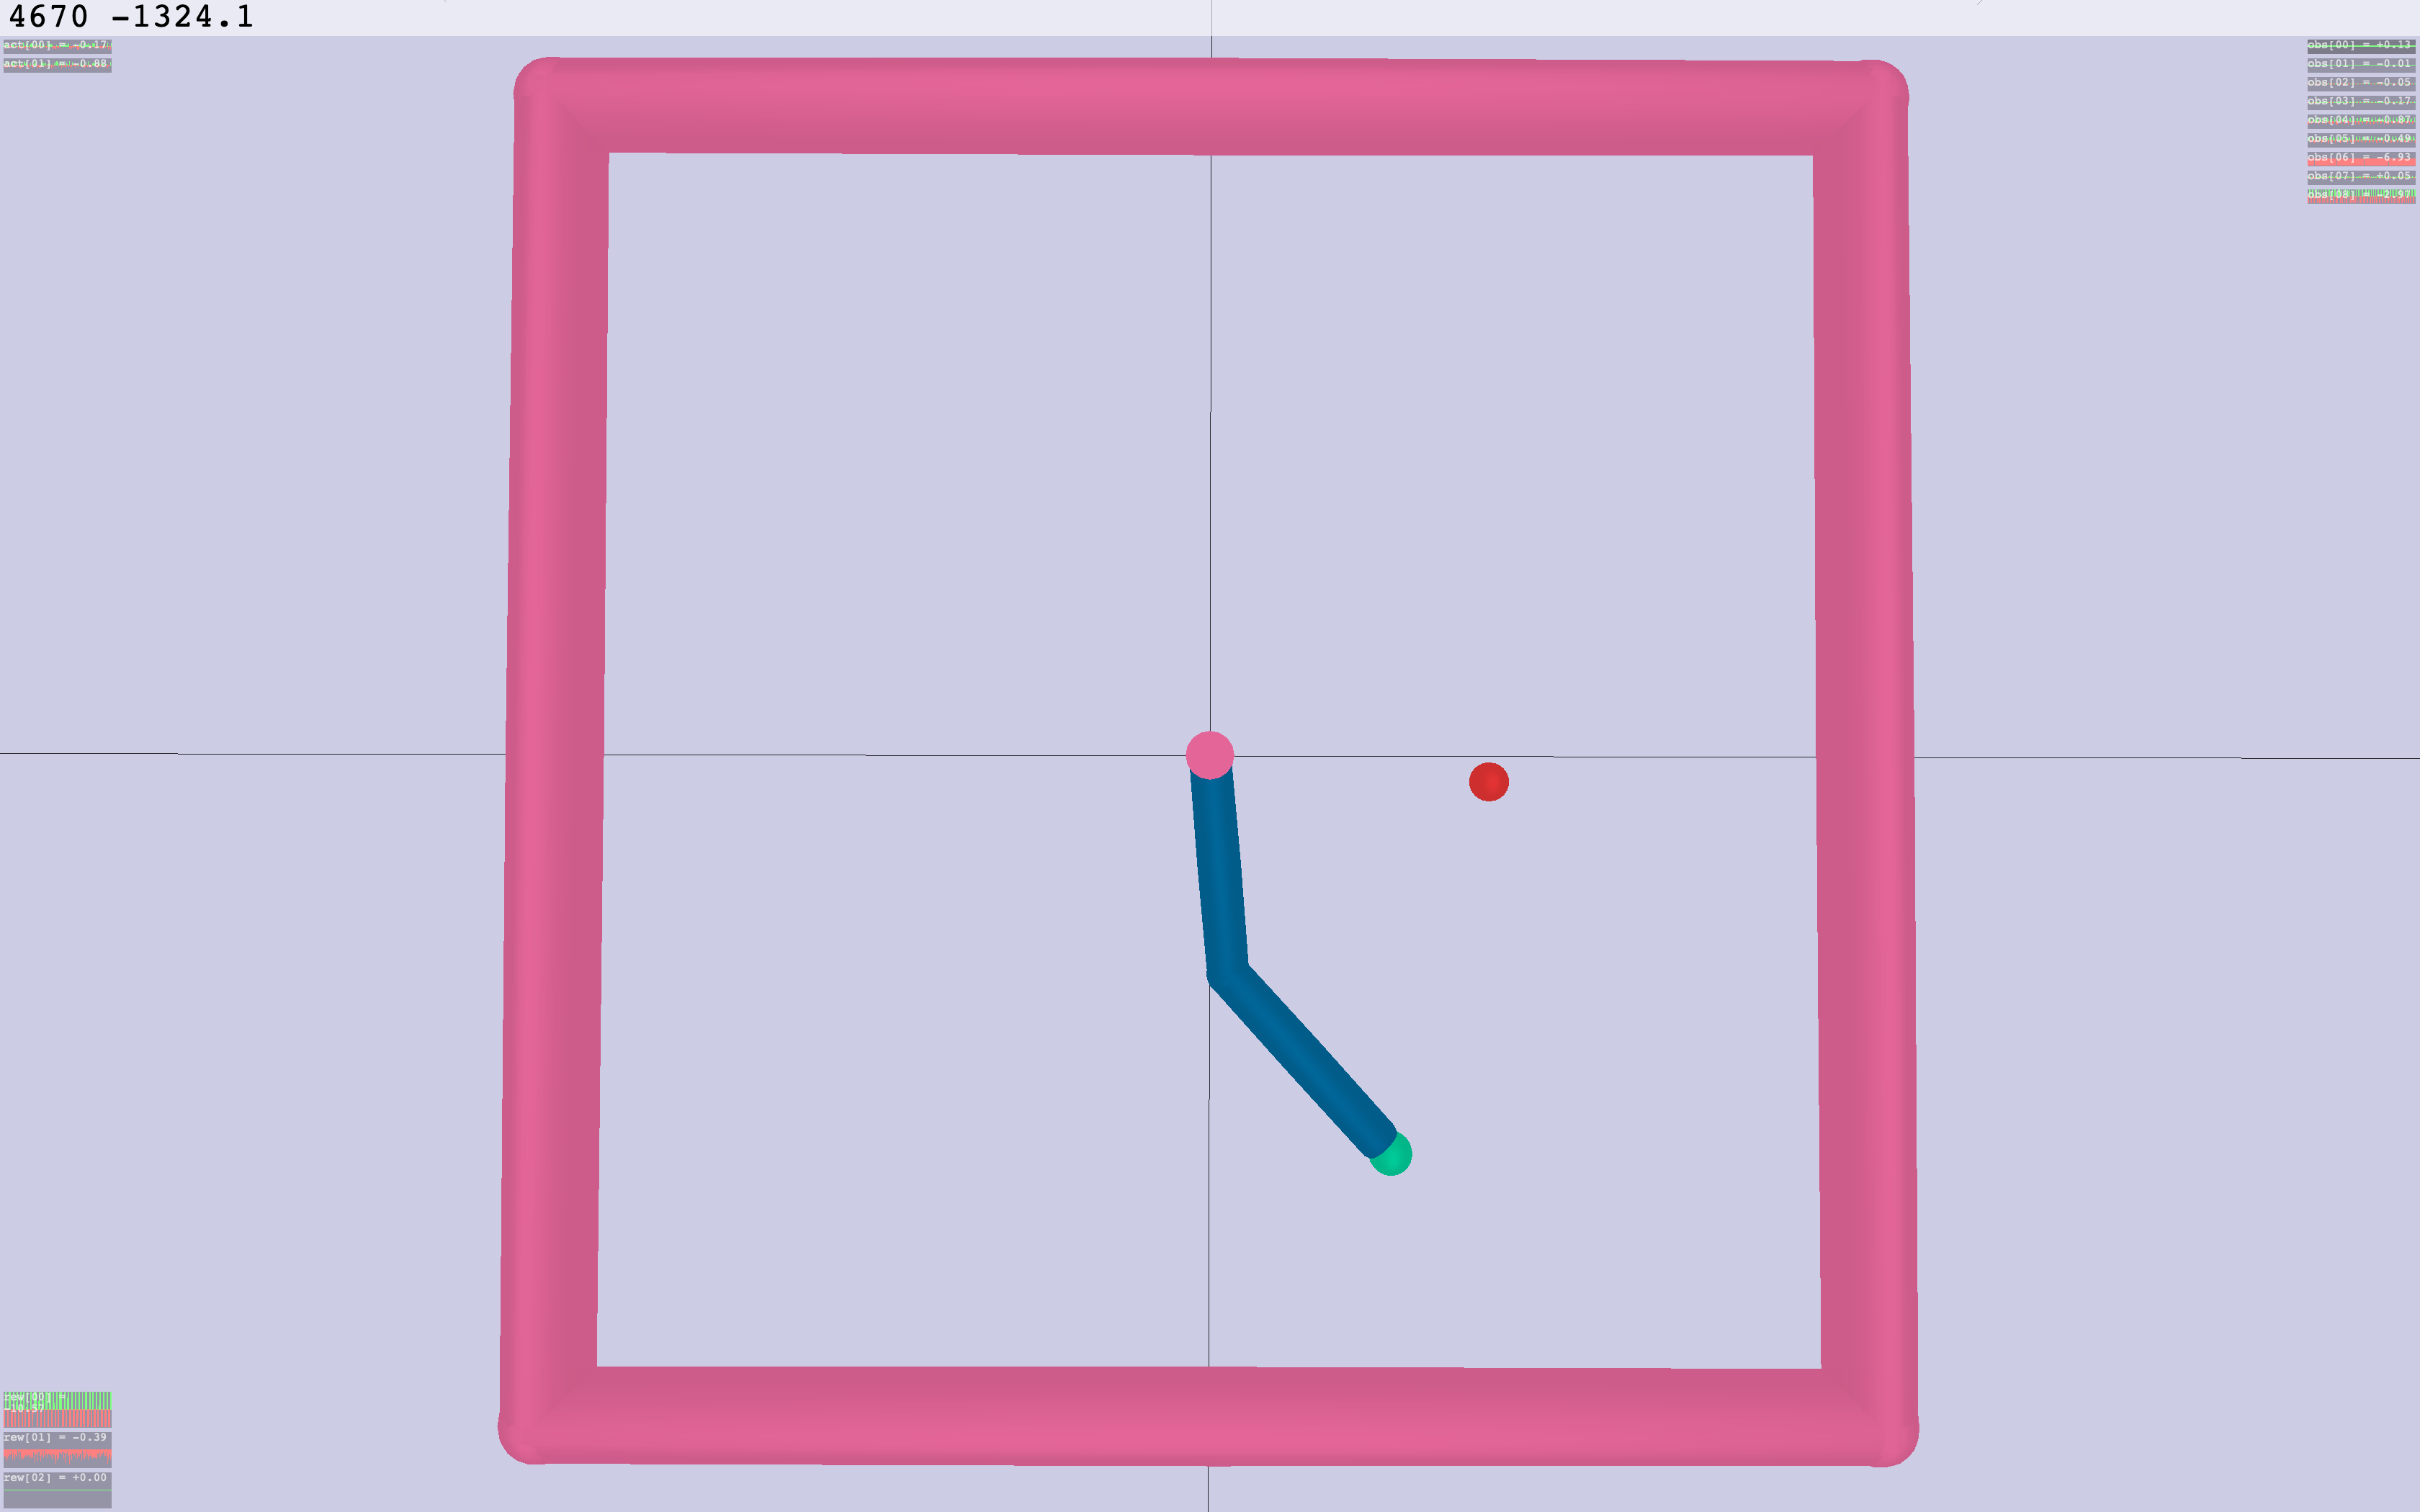
\includegraphics[width=0.7\linewidth]{figures/envs/openai_roboreacher.png}
            \caption{OpenAI Reacher Environment}
            \label{fig:openai_reacher}
    \end{center}
\end{figure}

\begin{table}[!htb]
    \centering
    \begin{subtable}{.4\linewidth}
        \centering
        \begin{tabular}{|c|c|}
        \hline
        \multicolumn{2}{|c|}{{\ul \textit{\textbf{Observation Space}}}}                                                                                   \\ \hline
        \multirow{2}{*}{\textbf{Target Position}}                                                                      & \textit{X Position}              \\ \cline{2-2} 
                                                                                                                    & \textit{Y Position}              \\ \hline
        \multirow{2}{*}{\textbf{Arm to Target Vector}}                                                                 & \textit{Position vector 0}       \\ \cline{2-2} 
                                                                                                                    & \textit{Position vector 1}       \\ \hline
        \multirow{2}{*}{\textbf{\begin{tabular}[c]{@{}c@{}}Current Relative Position\\ of Central Joint\end{tabular}}} & \textit{cosine of central joint} \\ \cline{2-2} 
                                                                                                                    & \textit{sine of central joint}   \\ \hline
        \multirow{2}{*}{\textbf{\begin{tabular}[c]{@{}c@{}}Current Relative Position\\ of Elbow Joint\end{tabular}}}   & \textit{cosine of elbow joint}   \\ \cline{2-2} 
                                                                                                                    & \textit{sine of elbow joint}     \\ \hline
        \end{tabular}
        \caption{Gym Reacher Observation Information}
        \label{tab:gym_reacher_obs}
    \end{subtable}%
    \hfill
    \begin{subtable}{.4\linewidth}
        \centering
        \begin{tabular}{|c|c|}
            \hline
            \multicolumn{2}{|c|}{{\ul \textit{\textbf{Action Space (Continuous)}}}}                             \\ \hline
            \multirow{2}{*}{\textbf{Center Joint Torque}} & \multirow{2}{*}{\textit{range(-1, 1)}} \\
                                                          &                                        \\ \hline
            \multirow{2}{*}{\textbf{Elbow Joint Torque}}  & \multirow{2}{*}{\textit{range(-1, 1)}} \\
                                                          &                                        \\ \hline
            \end{tabular}
            \caption{Gym Reacher Action Information}
            \label{tab:gym_reacher_actions}
    \end{subtable}%
    \caption{Gym Reacher Observation and Action Information}
\end{table}

the reward function is designed based on the distance between the arm and the target along with electricity cost of the torque and angular velocity of the arm with small epsilon amount in case of the joint is stuck. 

\clearpage

\textbf{Unity MLAgents: 2D and 3D Reacher Environment}

We have replicate the same openai gym reacher environment in unity to test the transferability between different physics engines, along with two 3d reacher environment (single and multi-agents) described below:

\textbf{Replicated Gym Env:}

\begin{figure}[H]
    \begin{center}
            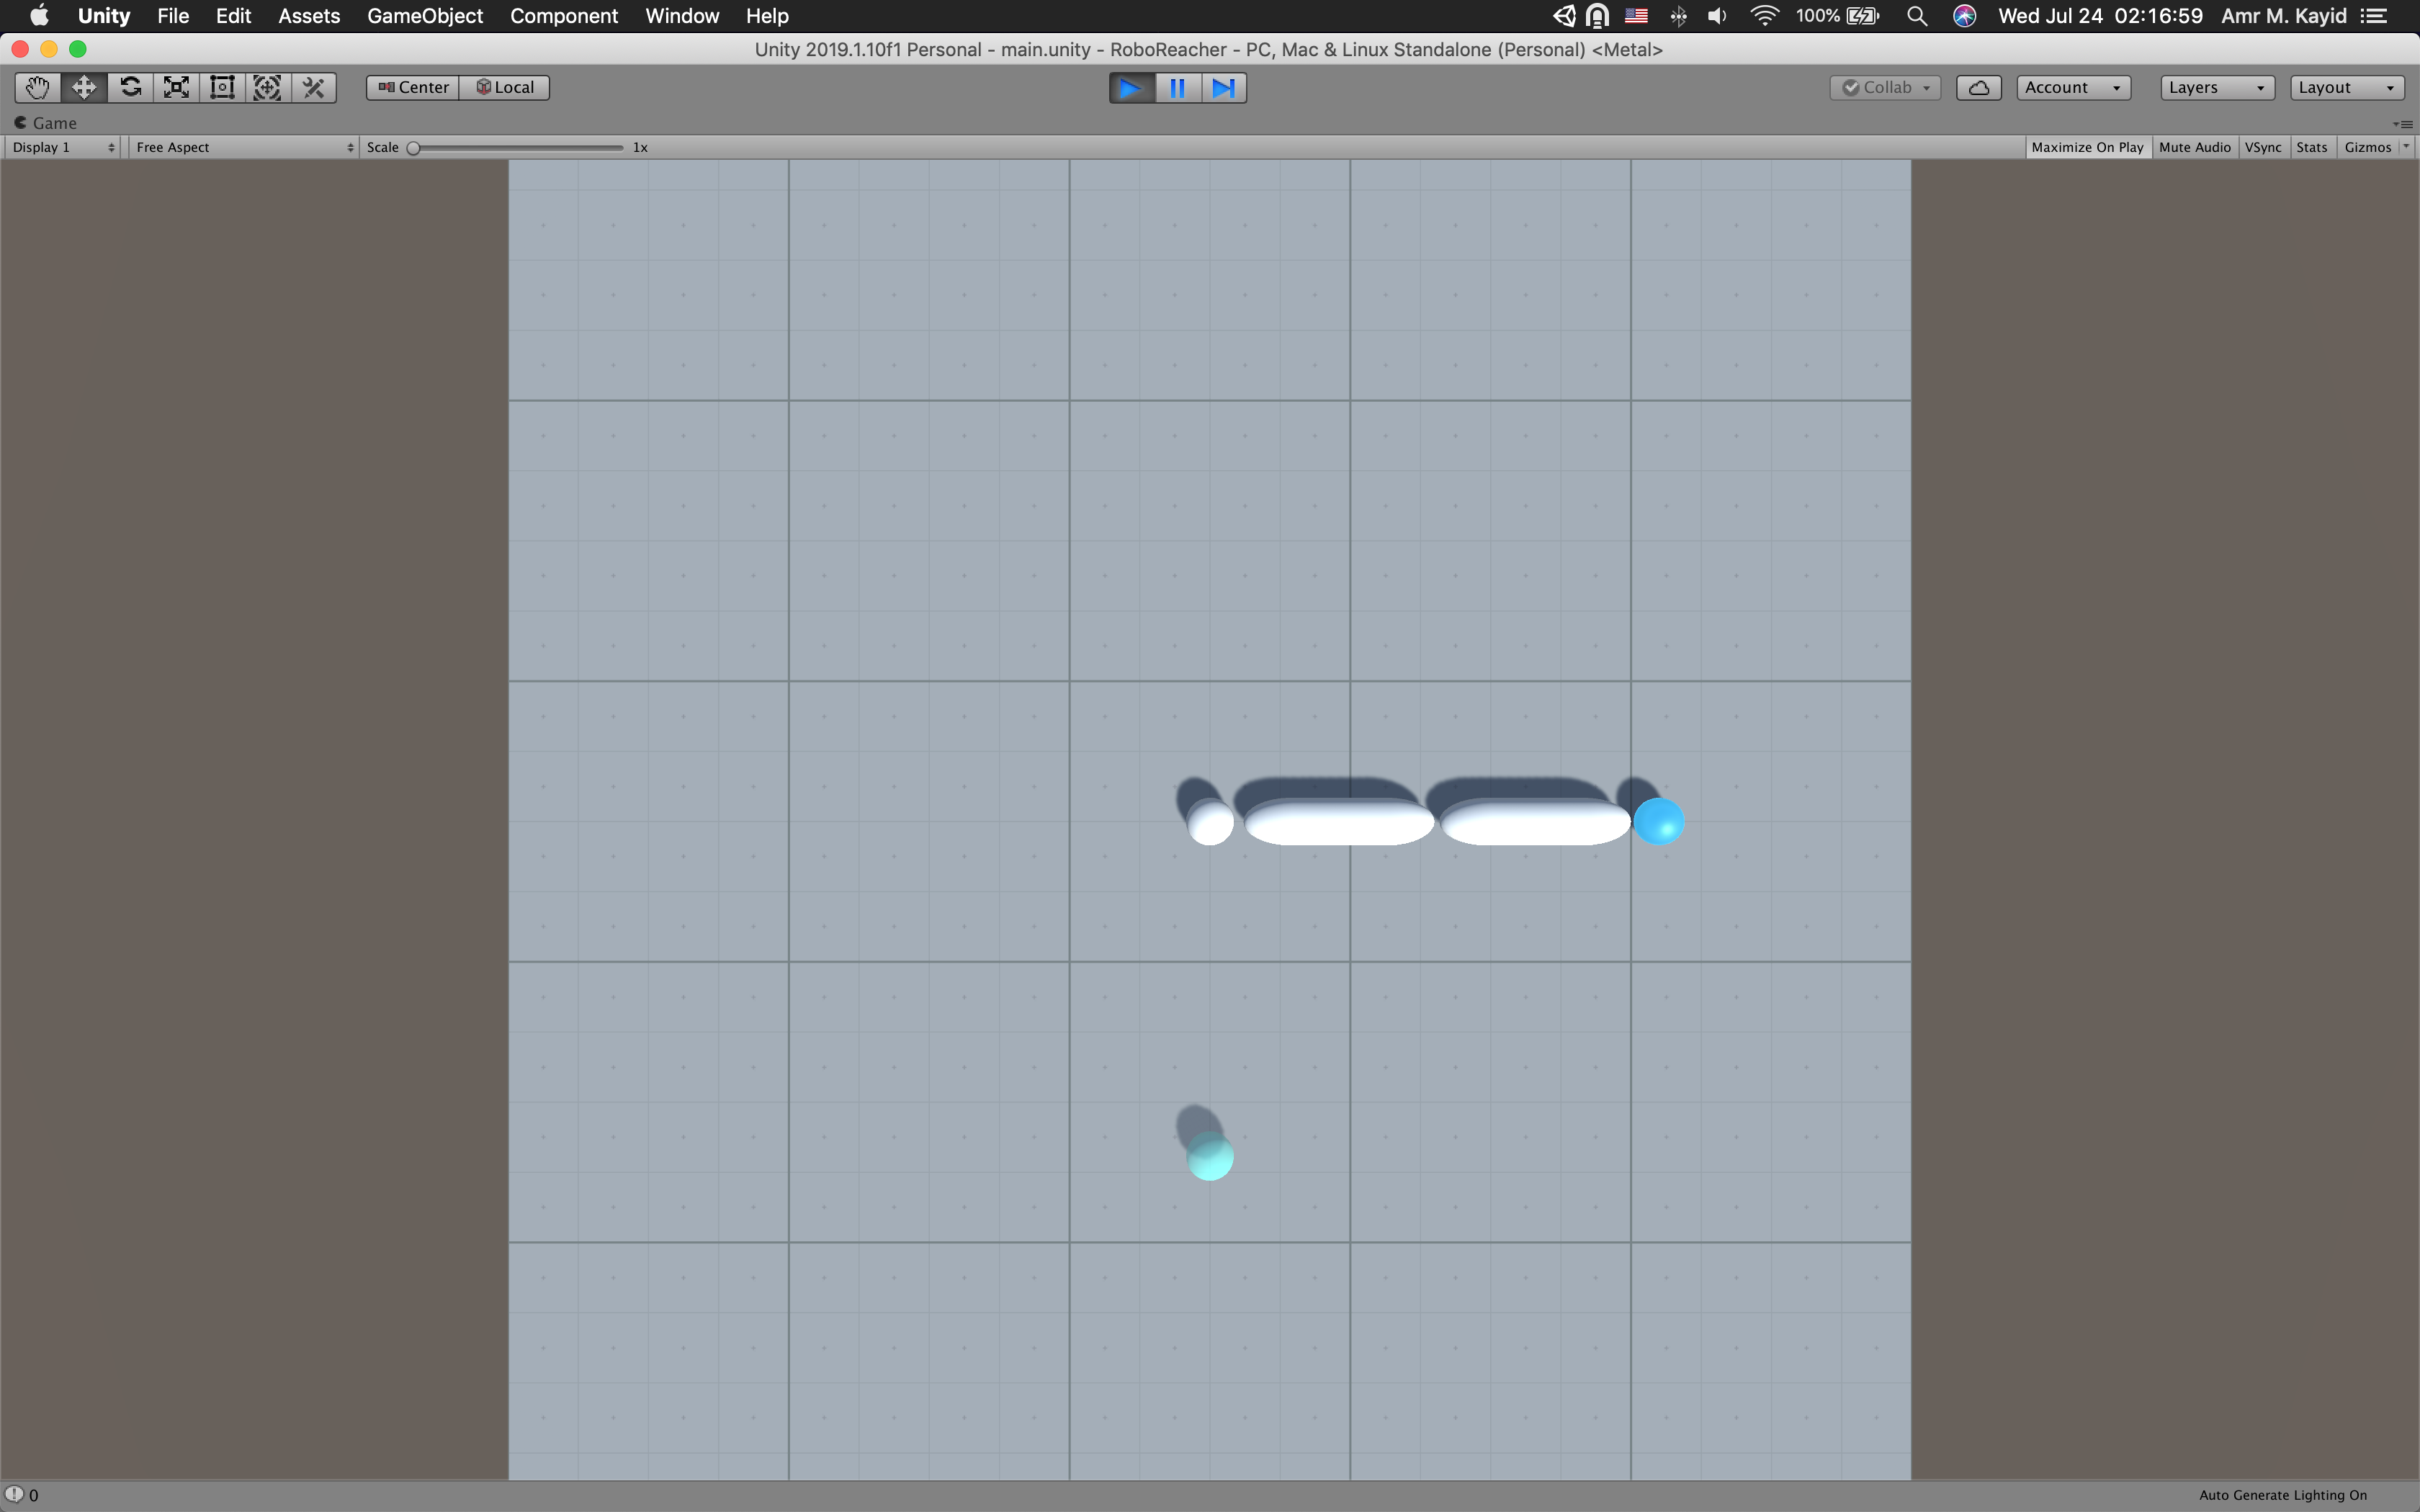
\includegraphics[width=0.7\linewidth]{figures/envs/unity_roboreacher.png}
            \caption{Replicated Gym Reacher Unity Environment}
            \label{fig:unity_reacher}
    \end{center}
\end{figure}


\textbf{Single Agent Reacher:} A robotic arm consist of two linked joints places in 3d plane surrounding it along with a moving sphere (target). The goal of the robotics arm it to reach target sphere and maintain following the point until the end of the episode. 

\begin{figure}[H]
    \begin{center}
            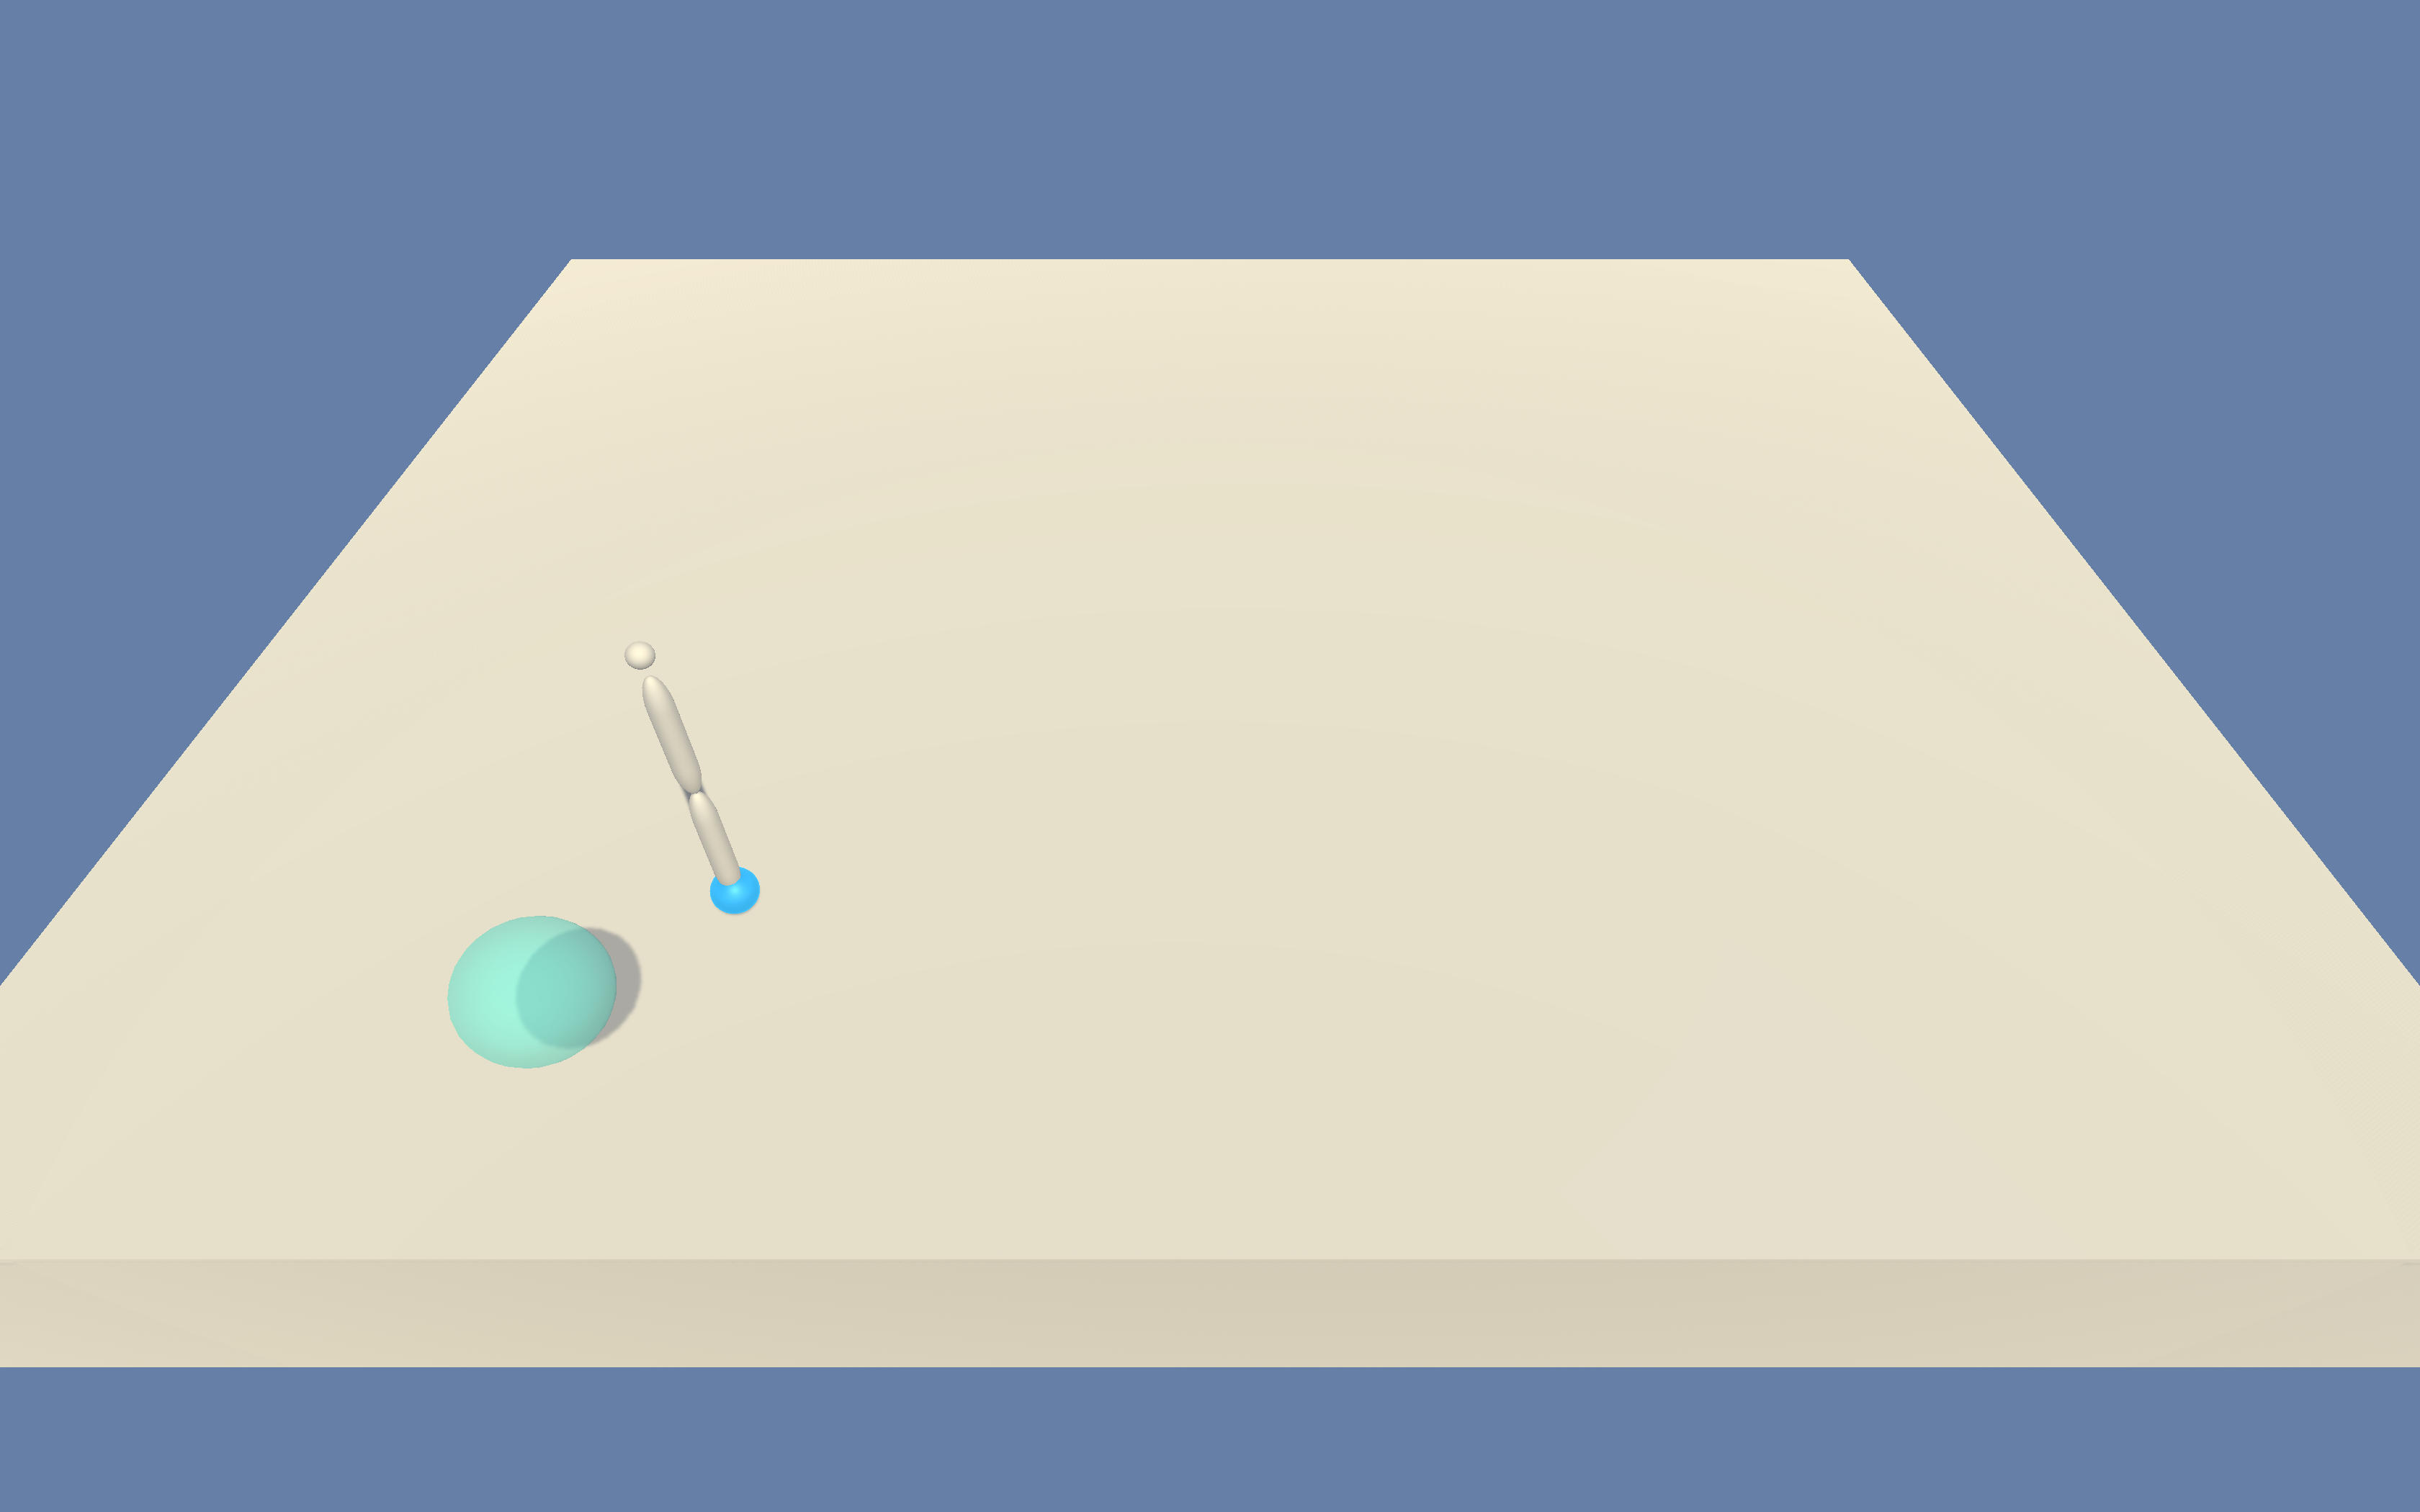
\includegraphics[width=0.7\linewidth]{figures/envs/unity_reacher_1.png}
            \caption{Unity Reacher Environment}
            \label{fig:unity_reacher_1}
    \end{center}
\end{figure}

\textbf{Multi-Agent Reacher:} in this environment, \textit{20 Agent} are used to parallelize the training process and collect more experiences and trajectories.

\begin{figure}[H]
    \begin{center}
            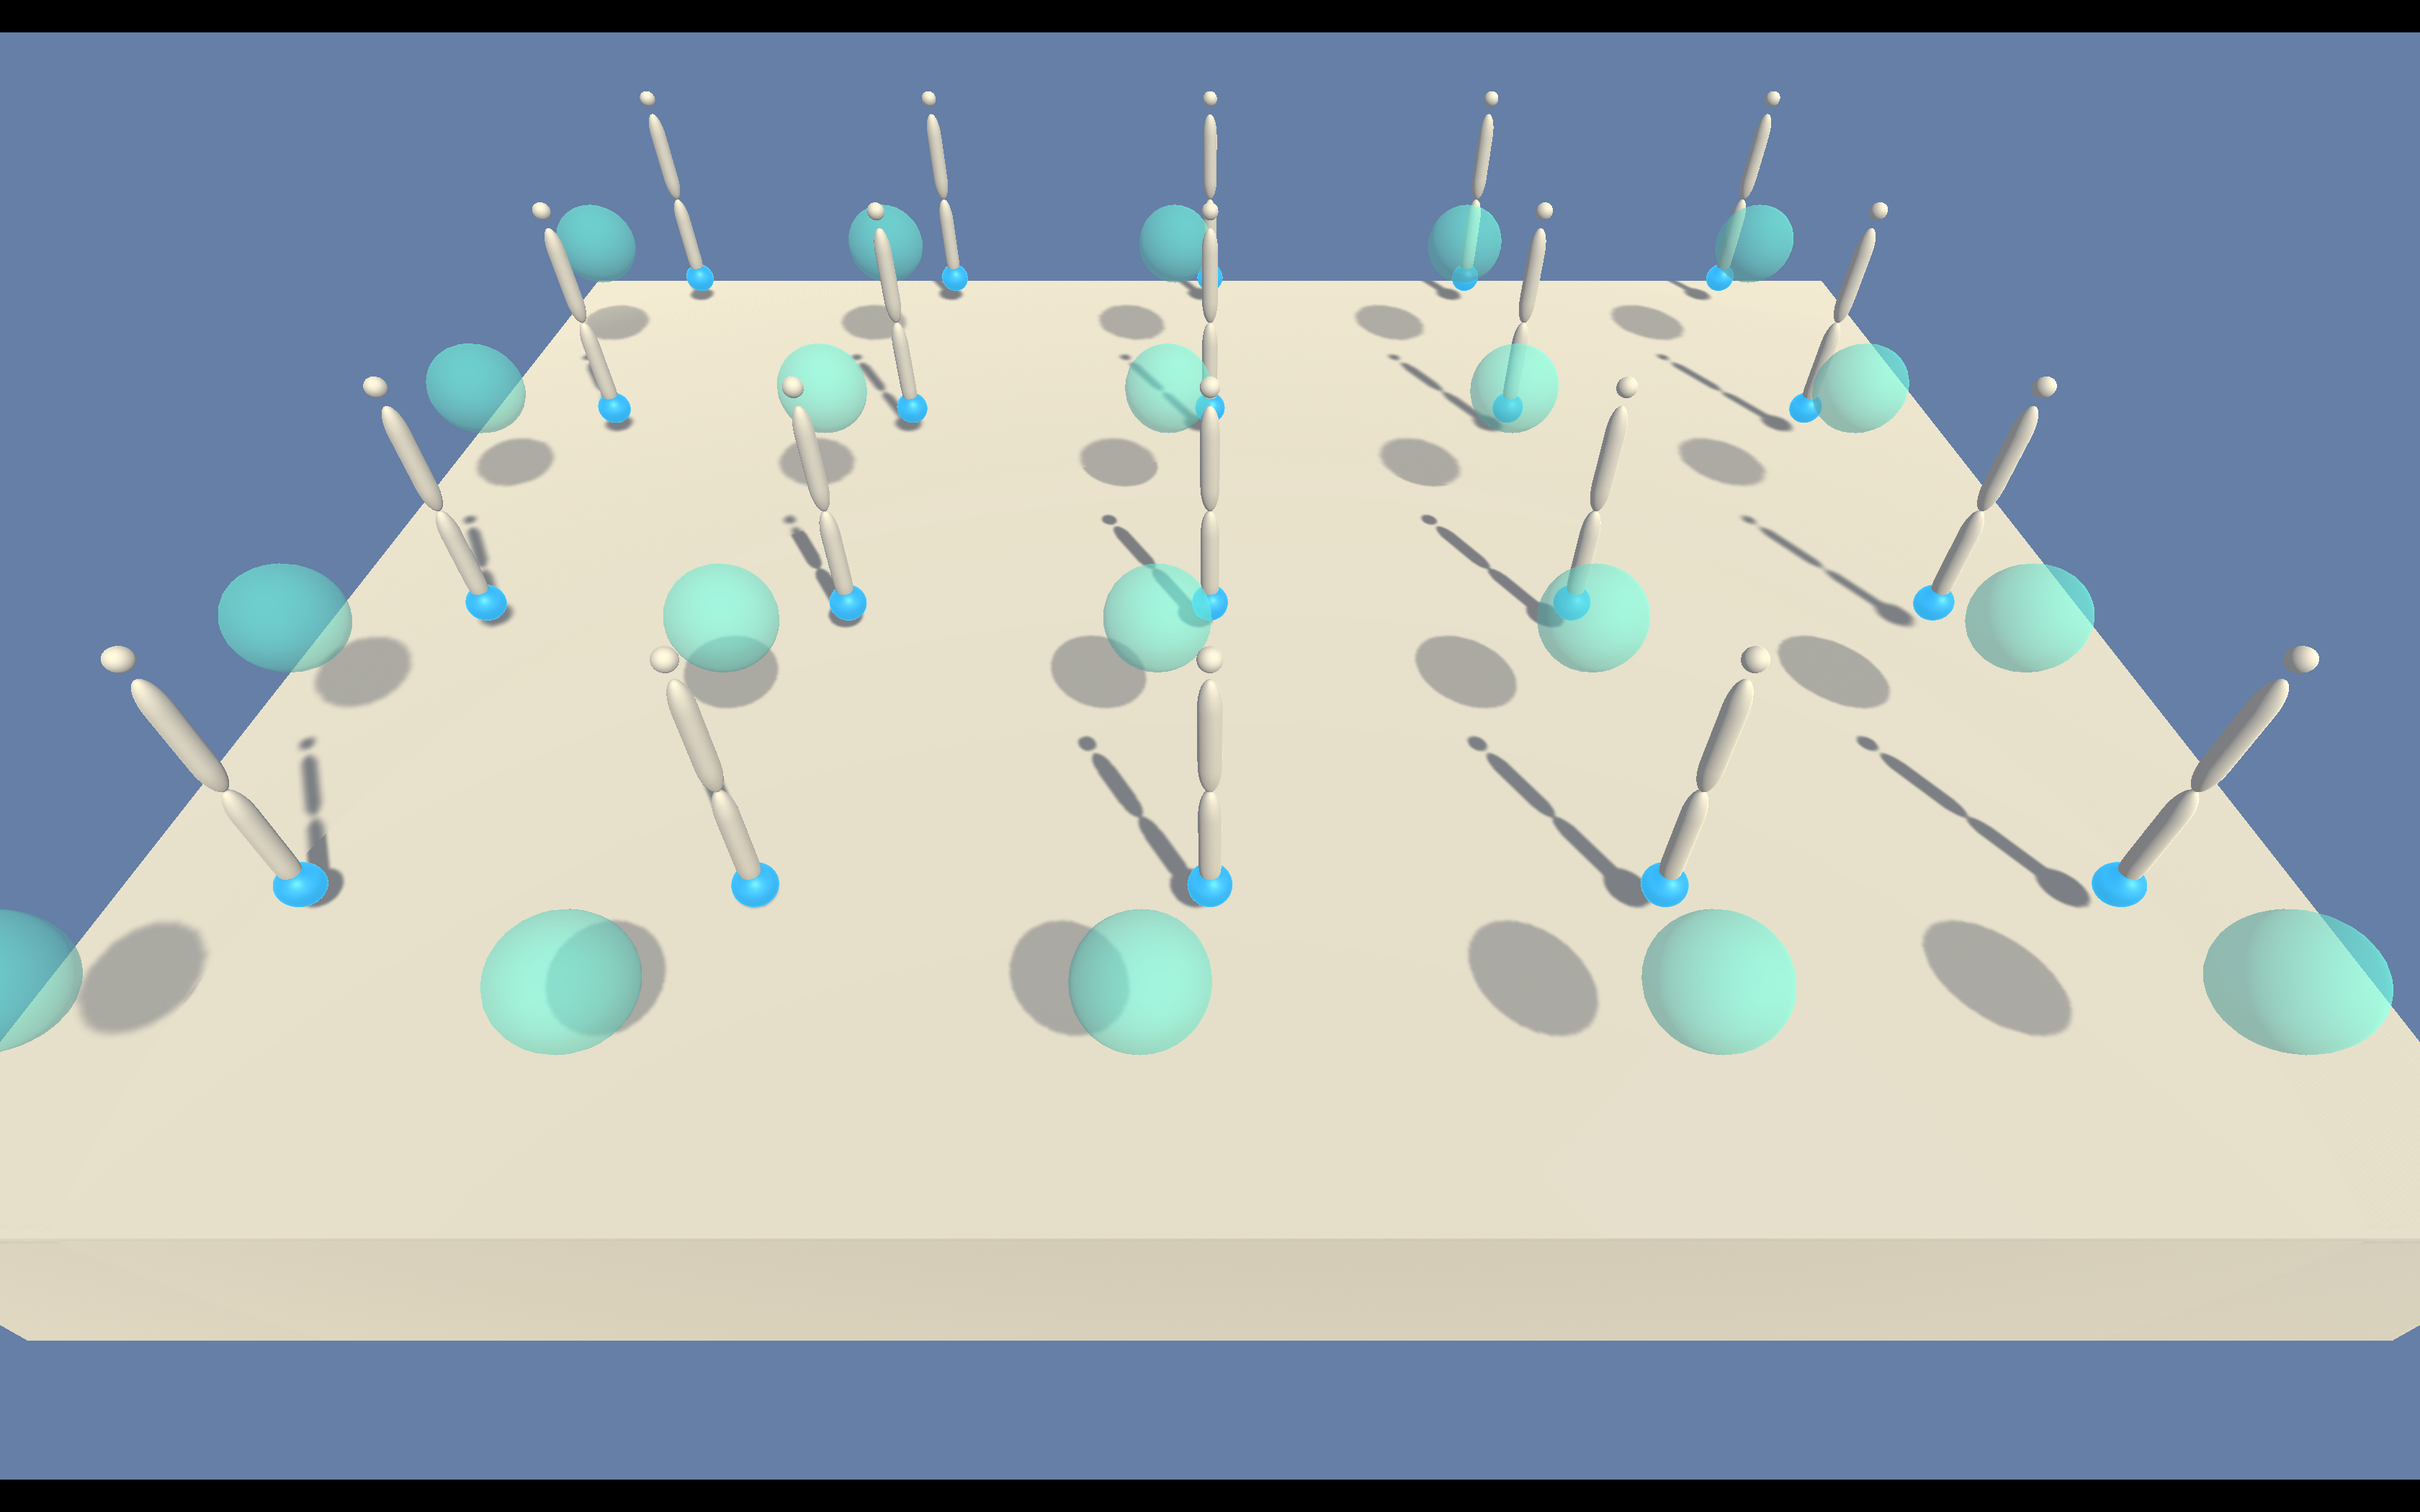
\includegraphics[width=0.7\linewidth]{figures/envs/unity_reacher_20.png}
            \caption{Unity Multi-Agent Reacher Environment}
            \label{fig:unity_reacher_20}
    \end{center}
\end{figure}

% !TeX root = ../../main.tex
% Add the above to each chapter to make compiling the PDF easier in some editors.

\chapter{Setup and Implementation}\label{chapter:setup_and_implementation}

In this chapter, the full details of the setups will be introduced. First, the used software framework will be presented. Then, our environments architecture and integration with the framework will be explained. Then, a brief description for the agents and algorithms will be shown. Lastly, description for all the used environments in our experiments will be provided.

\section{Overview}

Our approach is to setup a distributed learning architecture to run multiple experiments between selected environment and compare the results between training in normal non-distributed and distributed modes. We selected relatively close environment to robotics simulation with continuous observation and action spaces. A new abstract classes is introduced to run with the selected framework and unify the differences between different environments and physics simulators. A selection of the state of the art algorithms is used to train our reinforcement learning agents and compare between the algorithm and the modes for each algorithm.

\section{Software}
\textbf{Ray Framework~\parencite{moritz2018ray}: } Ray is a fast and simple framework for building and running distributed applications. The same code can be run on a single machine to achieve efficient multiprocessing, and it can be used on a cluster for large computations. Ray provide high scalability and a unified API for a variety of applications which is very useful for our experiments. Ray executes tasks asynchronously to achieve parallelism enabling us to run multiple environments in the same experiment to benefit from collection more experiences and trajectories for the agent.

\textbf{OpenAI Gym~\parencite{brockman2016openai}: } openai gym is a toolkit for developing and comparing reinforcement learning algorithms. It supports teaching agents everything from walking to playing games like Pong or Pinball. It has an open source interface to reinforcement learning tasks which provides an easy-to-use suite of reinforcement learning tasks. 

The core gym interface is \textbf{Env}, which is the unified environment interface. 
The following are the methods for the abstracted gym Env:

\begin{itemize}
    \item \textit{\textbf{\colorbox{gray!20}{reset(self)}}}: Reset the environment's state. Returns observation.
    \item \textit{\textbf{\colorbox{gray!20}{step(self, action)}}}: Step the environment by one time-step. Returns observation, reward, done, info.
    \item \textit{\textbf{\colorbox{gray!20}{render(self, mode='human')}}}: Render one frame of the environment. The default mode will do something human friendly, such as pop up a window.
\end{itemize}

\textbf{Unity MLAgents~\parencite{juliani2018unity}: } unity mlagents toolkit is an open-source Unity plugin that enables games and simulations to serve as environments for training intelligent agents. It has more realistic and complex simulation environments. It provides the ability to flexibly configure
the simulation. By taking advantage of Unity as a simulation platform, the toolkit enables the development of learning environments which are rich in sensory and physical complexity, provide compelling cognitive challenges, and support dynamic multi-agent interaction. Agents can be trained using reinforcement learning, imitation learning, neuroevolution, or other machine learning methods through a simple-to-use Python API. They provide implementations of state-of-the-art algorithms to enable game developers and hobbyists to easily train intelligent agents for 2D, 3D and VR/AR games. We are using this to test running multiple agents in the same environment and compare the effect with one agent only. Also, to experiment the transferability between different physics simulators.

\section{Architecture}

At a high level, ray provides an \textbf{\colorbox{gray!20}{Trainer}} class which holds a policy for environment interaction. Through the trainer interface~\ref{fig:ray_trainer}, the policy can be trained, check-pointed, or an action computed. In multi-agent training, the trainer manages the querying and optimization of multiple policies at once. It provides custom resources configurations~\ref{fig:ray_config}, which can control the degree of parallelism used by setting the \colorbox{gray!20}{\texttt{num\_workers}} hyper-parameter for most algorithms. The number of GPUs the driver should use can be set via the \colorbox{gray!20}{\texttt{num\_gpus}} option. Similarly, the resource allocation to workers can be controlled via \colorbox{gray!20}{\texttt{num\_cpus\_per\_worker}}, \colorbox{gray!20}{\texttt{num\_gpus\_per\_worker}}, and \colorbox{gray!20}{\texttt{custom\_resources\_per\_worker}}. The number of GPUs can be a fractional quantity to allocate only a fraction of a GPU. For example, with DQN you can pack five trainers onto one GPU by setting \colorbox{gray!20}{\texttt{num\_gpus}: 0.2}.

\begin{figure}[H]
	\centering
	\begin{subfigure}[b]{0.4\textwidth}
		\centering
		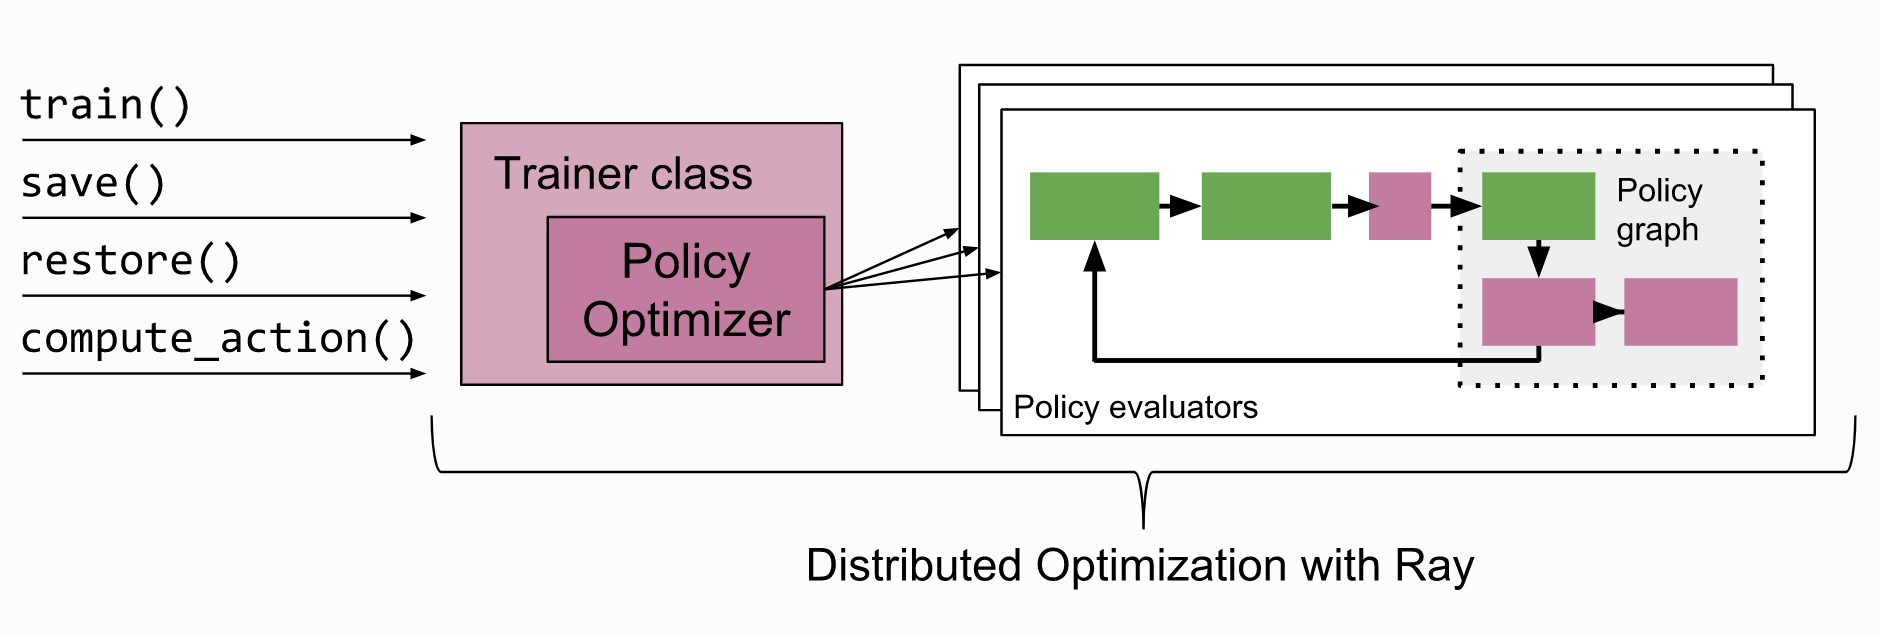
\includegraphics[width=\textwidth]{figures/architecture/ray_trainer.png}
		\caption{Ray Training Process}
		\label{fig:ray_trainer}
    \end{subfigure}
    \hfill
	\begin{subfigure}[b]{0.4\textwidth}
		\centering
		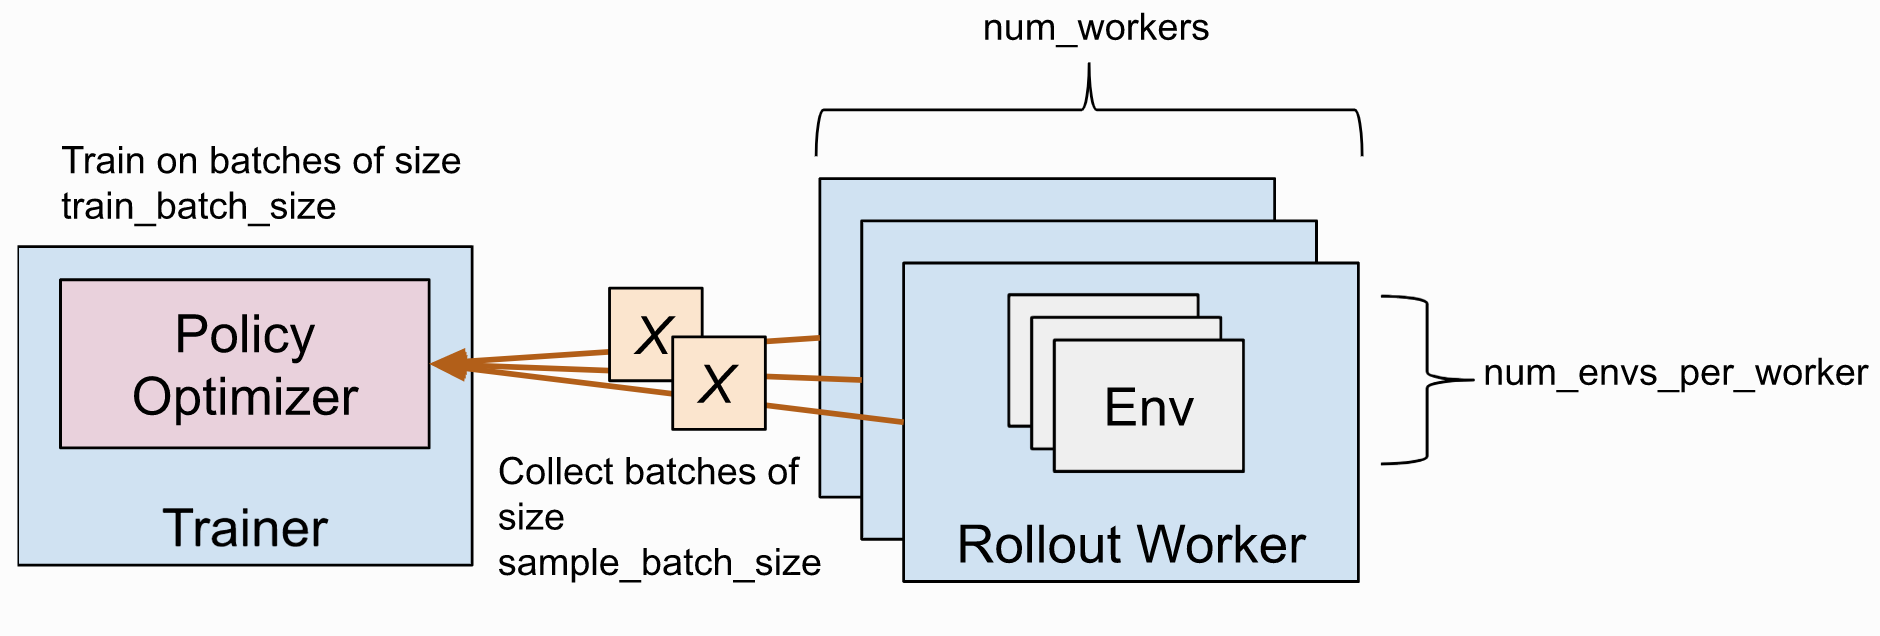
\includegraphics[width=\textwidth]{figures/architecture/ray_config.png}
        \caption{Ray Configurable resources}
		\label{fig:ray_config}
	\end{subfigure}
	\hfill
	   \caption{General Overview of Ray framework~\parencite{moritz2018ray}}
	   \label{fig:ray}
\end{figure}

Since ray support only OpenAI Gym environments along with their provided multi-agent and also batched environments, we had to implement our custom environment to unify between unity mlagents and openai gym environments. Also, we implemented our custom Multi-Agent environments for both used environments as shown in the following figure~\ref{fig:ray_envs}.

\begin{figure}[H]
	\centering
		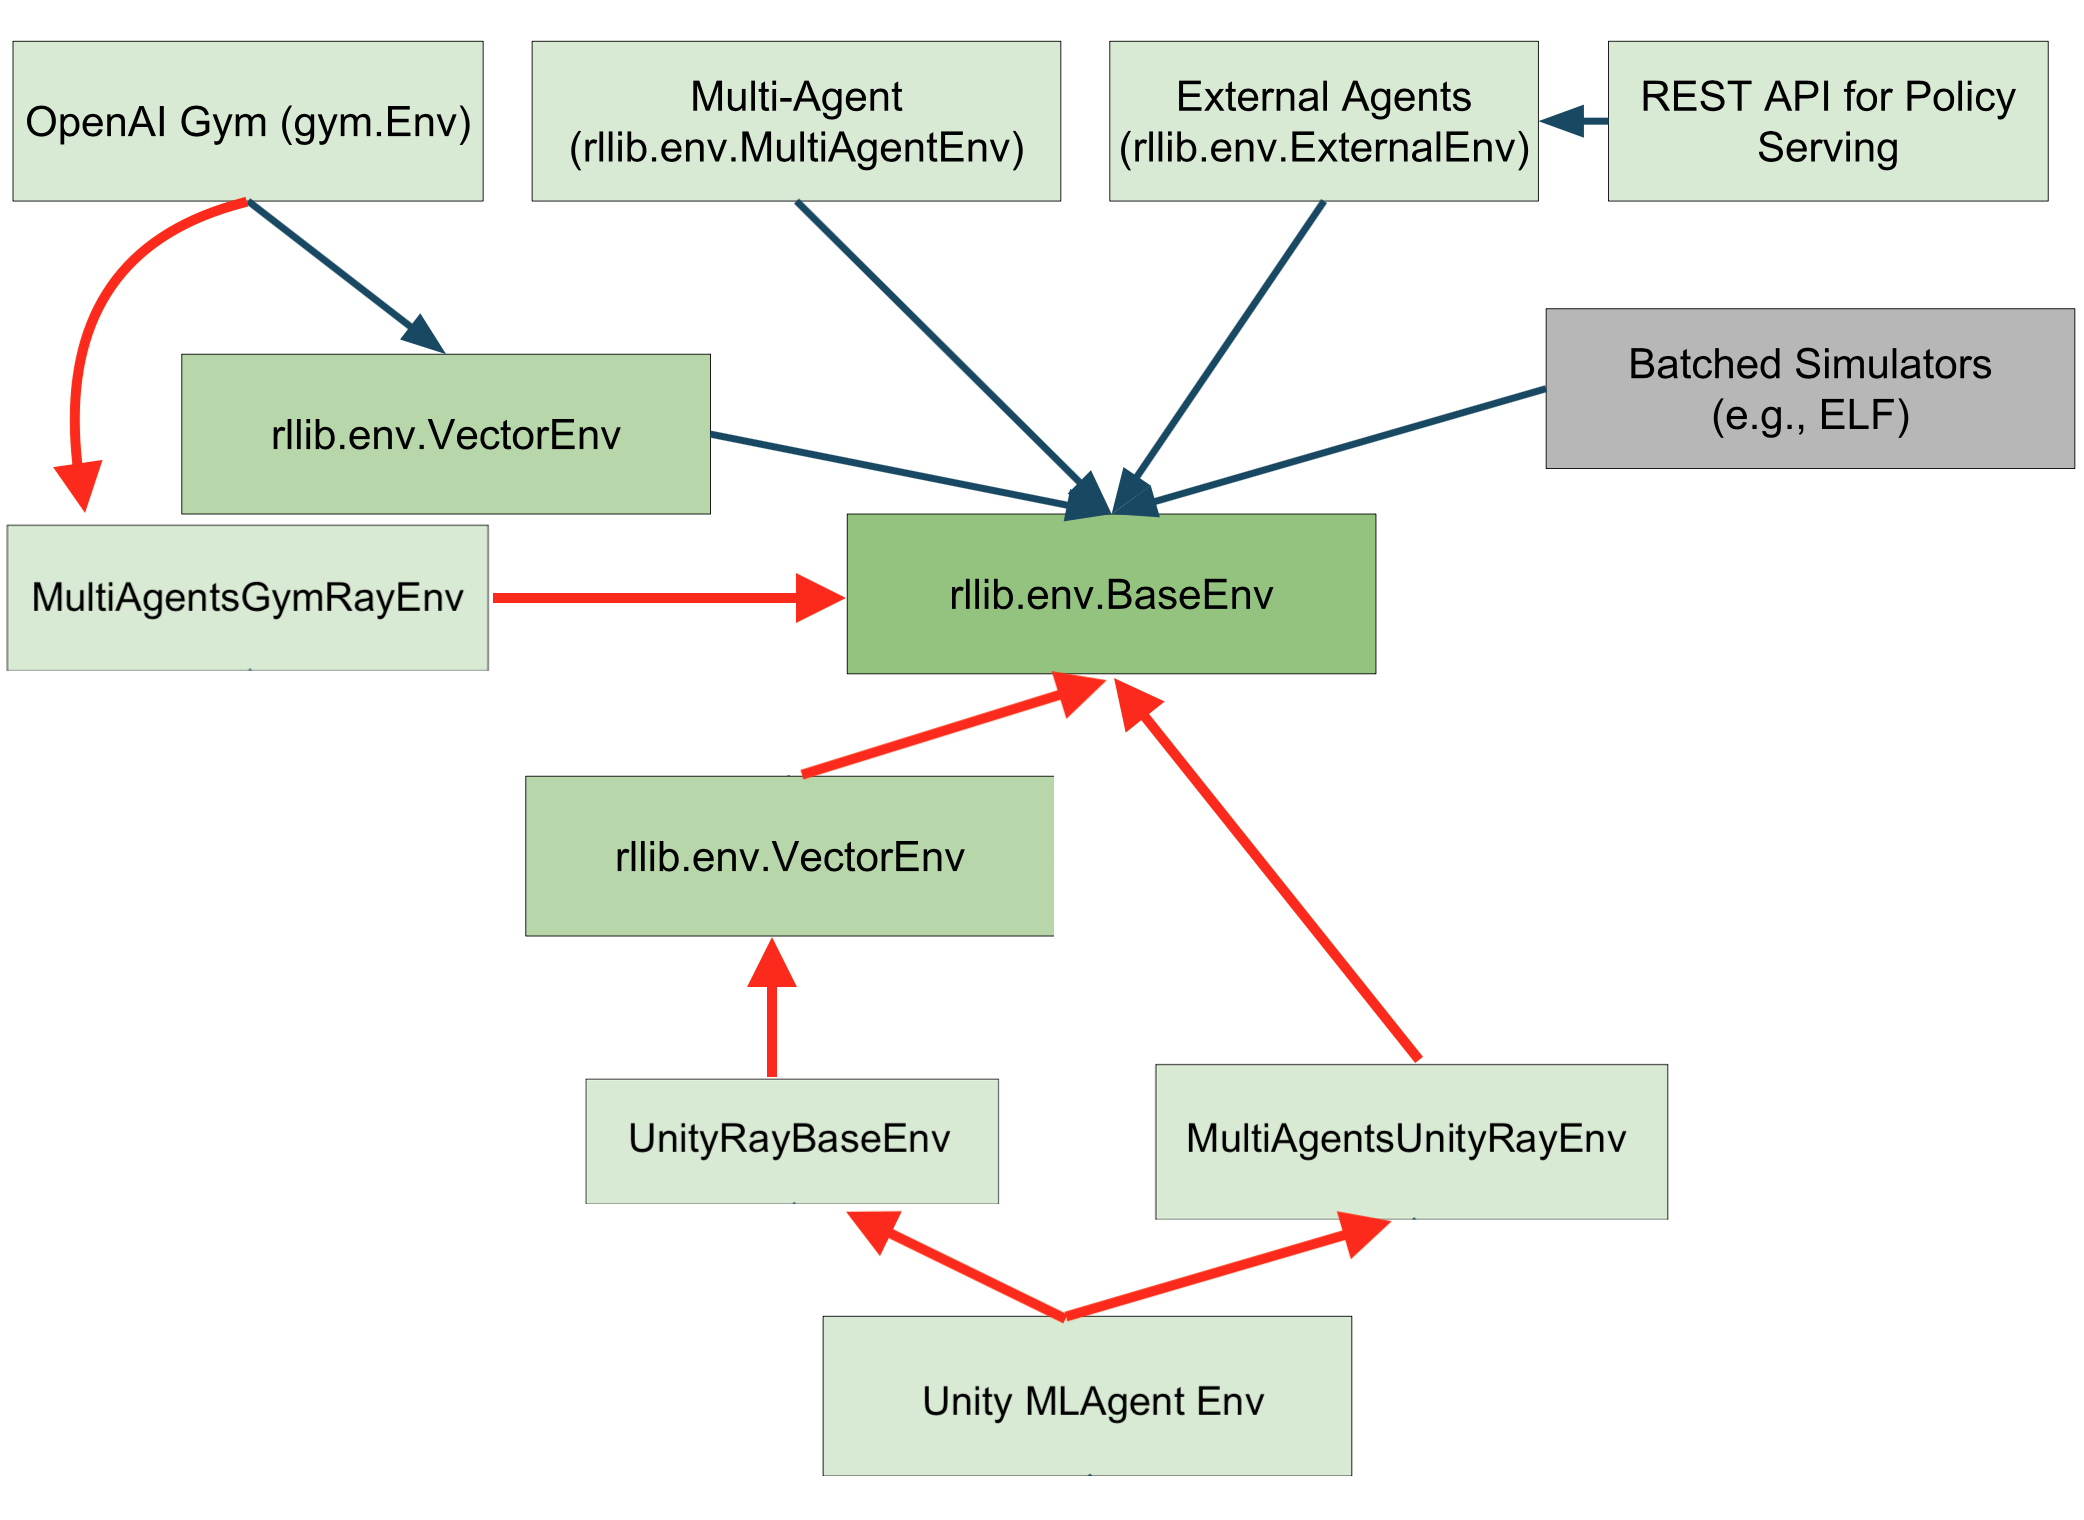
\includegraphics[width=\linewidth]{figures/architecture/ray_envs.png}
		\caption{Our Custom Environments}
		\label{fig:ray_envs}
\end{figure}

\clearpage

Custom environments implementations and methods are described below:

\textbf{UnityRayEnv}:\\
our base unity environment maps the observations and actions from unity mlagents toolkit to be compatible with Ray BaseEnv. Since unity mlagents deals with brains that control the agents and the environments we had to convert it to the required \colorbox{gray!20}{\texttt{observation\_space}} and \colorbox{gray!20}{\texttt{action\_space}} for ray env with the following methods:
\begin{itemize}
    \item \textit{\textbf{\colorbox{gray!20}{\texttt{\_\_init\_\_(self)}}}}: Create the unity environment from the unity build env, convert the observation and action spaces to be ray-compatible.
    \item \textit{\textbf{\colorbox{gray!20}{reset(self)}}}: Reset the environment's state. Returns observation.
    \item \textit{\textbf{\colorbox{gray!20}{step(self, action)}}}: Step the environment by one time-step. Returns observation, reward, done, info.
\end{itemize}

\textbf{MultiAgentsUnityRayEnv}:\\
this class inherit from both \colorbox{gray!20}{\textbf{UnityRayEnv}} and \colorbox{gray!20}{\textbf{MultiAgentEnv}}~\ref{fig:ray_multiagentenv}. The difference from the base environment is in both methods \textit{\textbf{\colorbox{gray!20}{reset(self)}}} and \textit{\textbf{\colorbox{gray!20}{step(self, \texttt{actions\_dict})}}}, where the reset function reset all the observations for each agent that exist in the environment and step function take a dictionary of actions corresponding for each action of a single agent. The same applies to \textbf{MultiAgentsGymRayEnv}.

\begin{figure}[H]
	\centering
		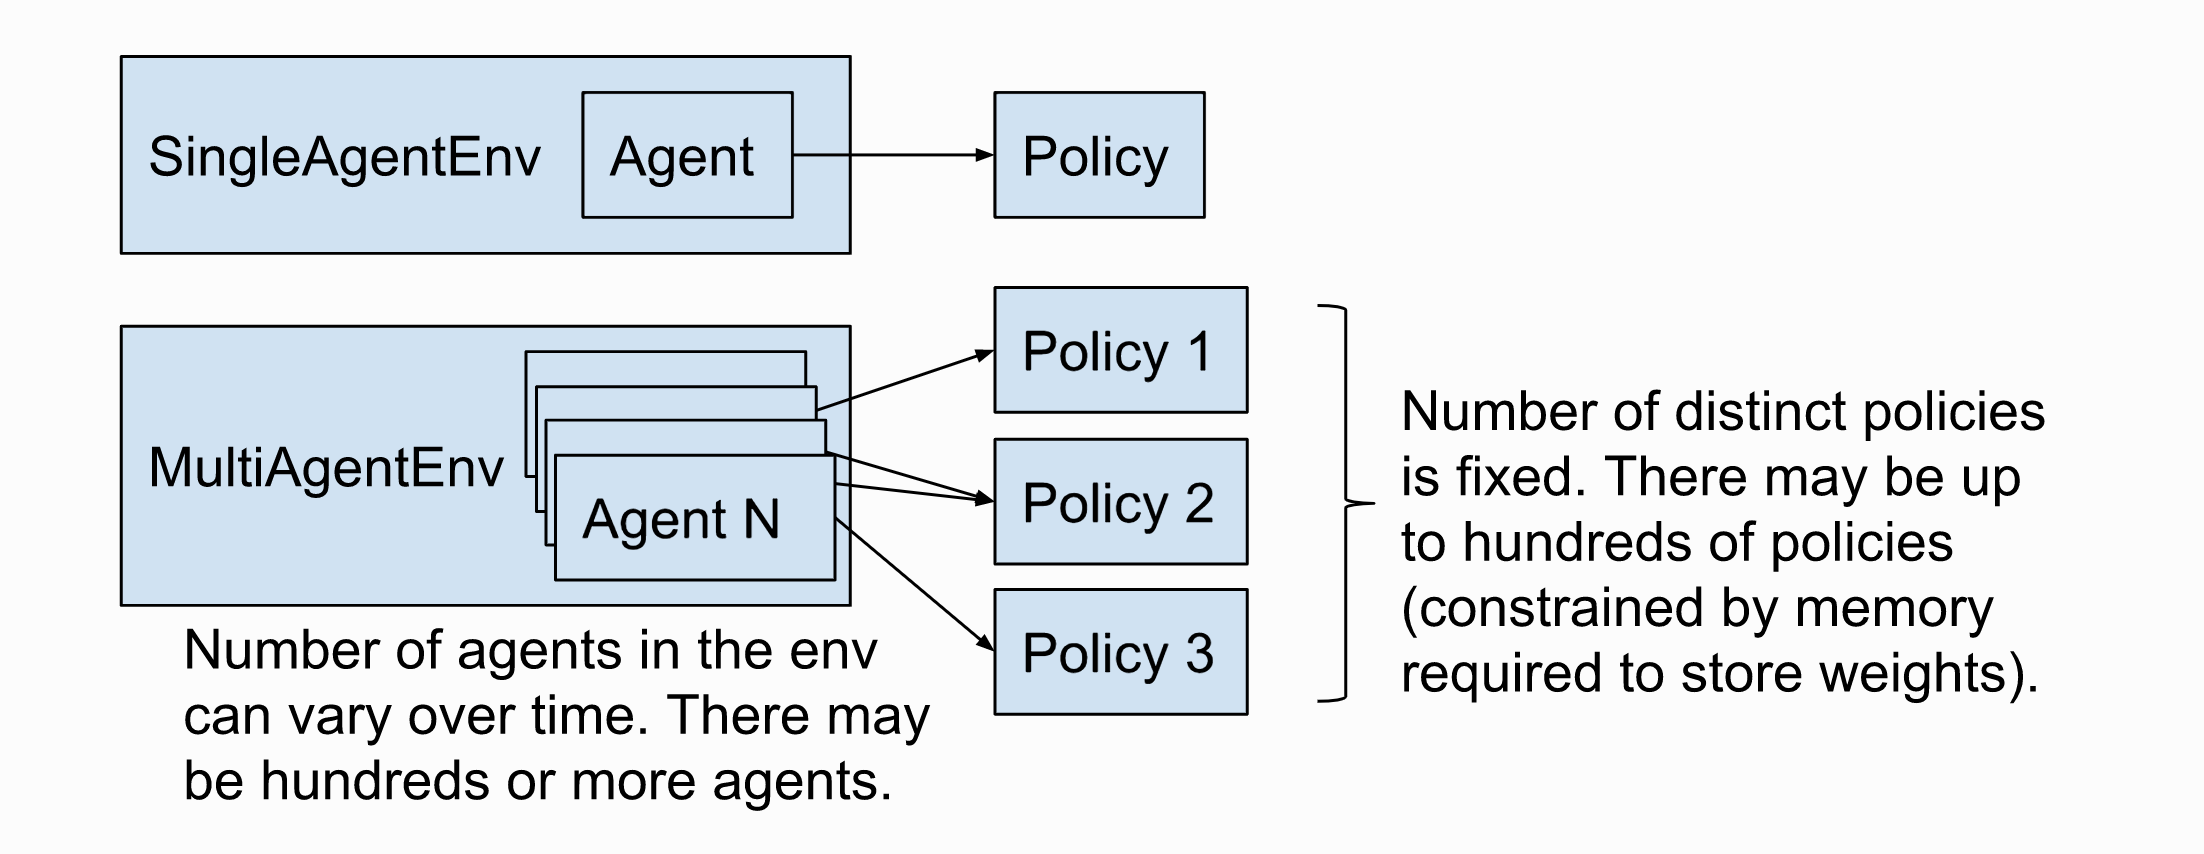
\includegraphics[width=\linewidth]{figures/architecture/ray_multiagentenv.png}
		\caption{Ray MultiAgentEnv}
		\label{fig:ray_multiagentenv}
\end{figure}

\section{Agents and Algorithms}

\begin{itemize}
    \item \textbf{Proximal Policy Optimization (PPO)}: PPO’s clipped objective supports multiple SGD passes over the same batch of experiences. RLlib’s multi-GPU optimizer pins that data in GPU memory to avoid unnecessary transfers from host memory, substantially improving performance over a naive implementation. RLlib’s PPO scales out using multiple workers for experience collection, and also with multiple GPUs for SGD.

    \item \textbf{Distributed Prioritized Experience Replay (Ape-X)}: Ape-X variations of DQN, DDPG, use a single GPU learner and many CPU workers for experience collection. Experience collection can scale to hundreds of CPU workers due to the distributed prioritization of experience prior to storage in replay buffers.

    \item \textbf{Importance Weighted Actor-Learner Architecture (IMPALA)}: In IMPALA, a central learner runs SGD in a tight loop while asynchronously pulling sample batches from many actor processes. RLlib’s IMPALA implementation uses DeepMind’s reference V-trace code. Note that we do not provide a deep residual network out of the box, but one can be plugged in as a custom model. Multiple learner GPUs and experience replay are also supported.
\end{itemize}

\section{Environments and Tasks Description}
Our task is robotic related task, where we have a robotic arm consist of two linked joints \textit{(agent)} and moving sphere \textit{(target)}. The robotic arm and the goal differ according to the environment used. We have a one experiment where is the agent movement is in 2D and the goal of the agent it to reach the target as fast as possible to maximize the given cumulative reward. In the second experiment, the agent can move in 3D and the goal is to keep track of the moving target and move with it along the 3D space.

Following is detailed description for all the environment used in our experiments.

\textbf{OpenAI: Reacher Environment}

Our first and baseline environment is \textit{Reacher Environment}~\ref{fig:openai_reacher}: A robotic arm consist of two linked joints places in a squared arena surrounding it along with a moving sphere (target). The goal of the robotics arm it to reach target sphere and maintain following the point until the end of the episode. 

\begin{figure}[H]
    \begin{center}
            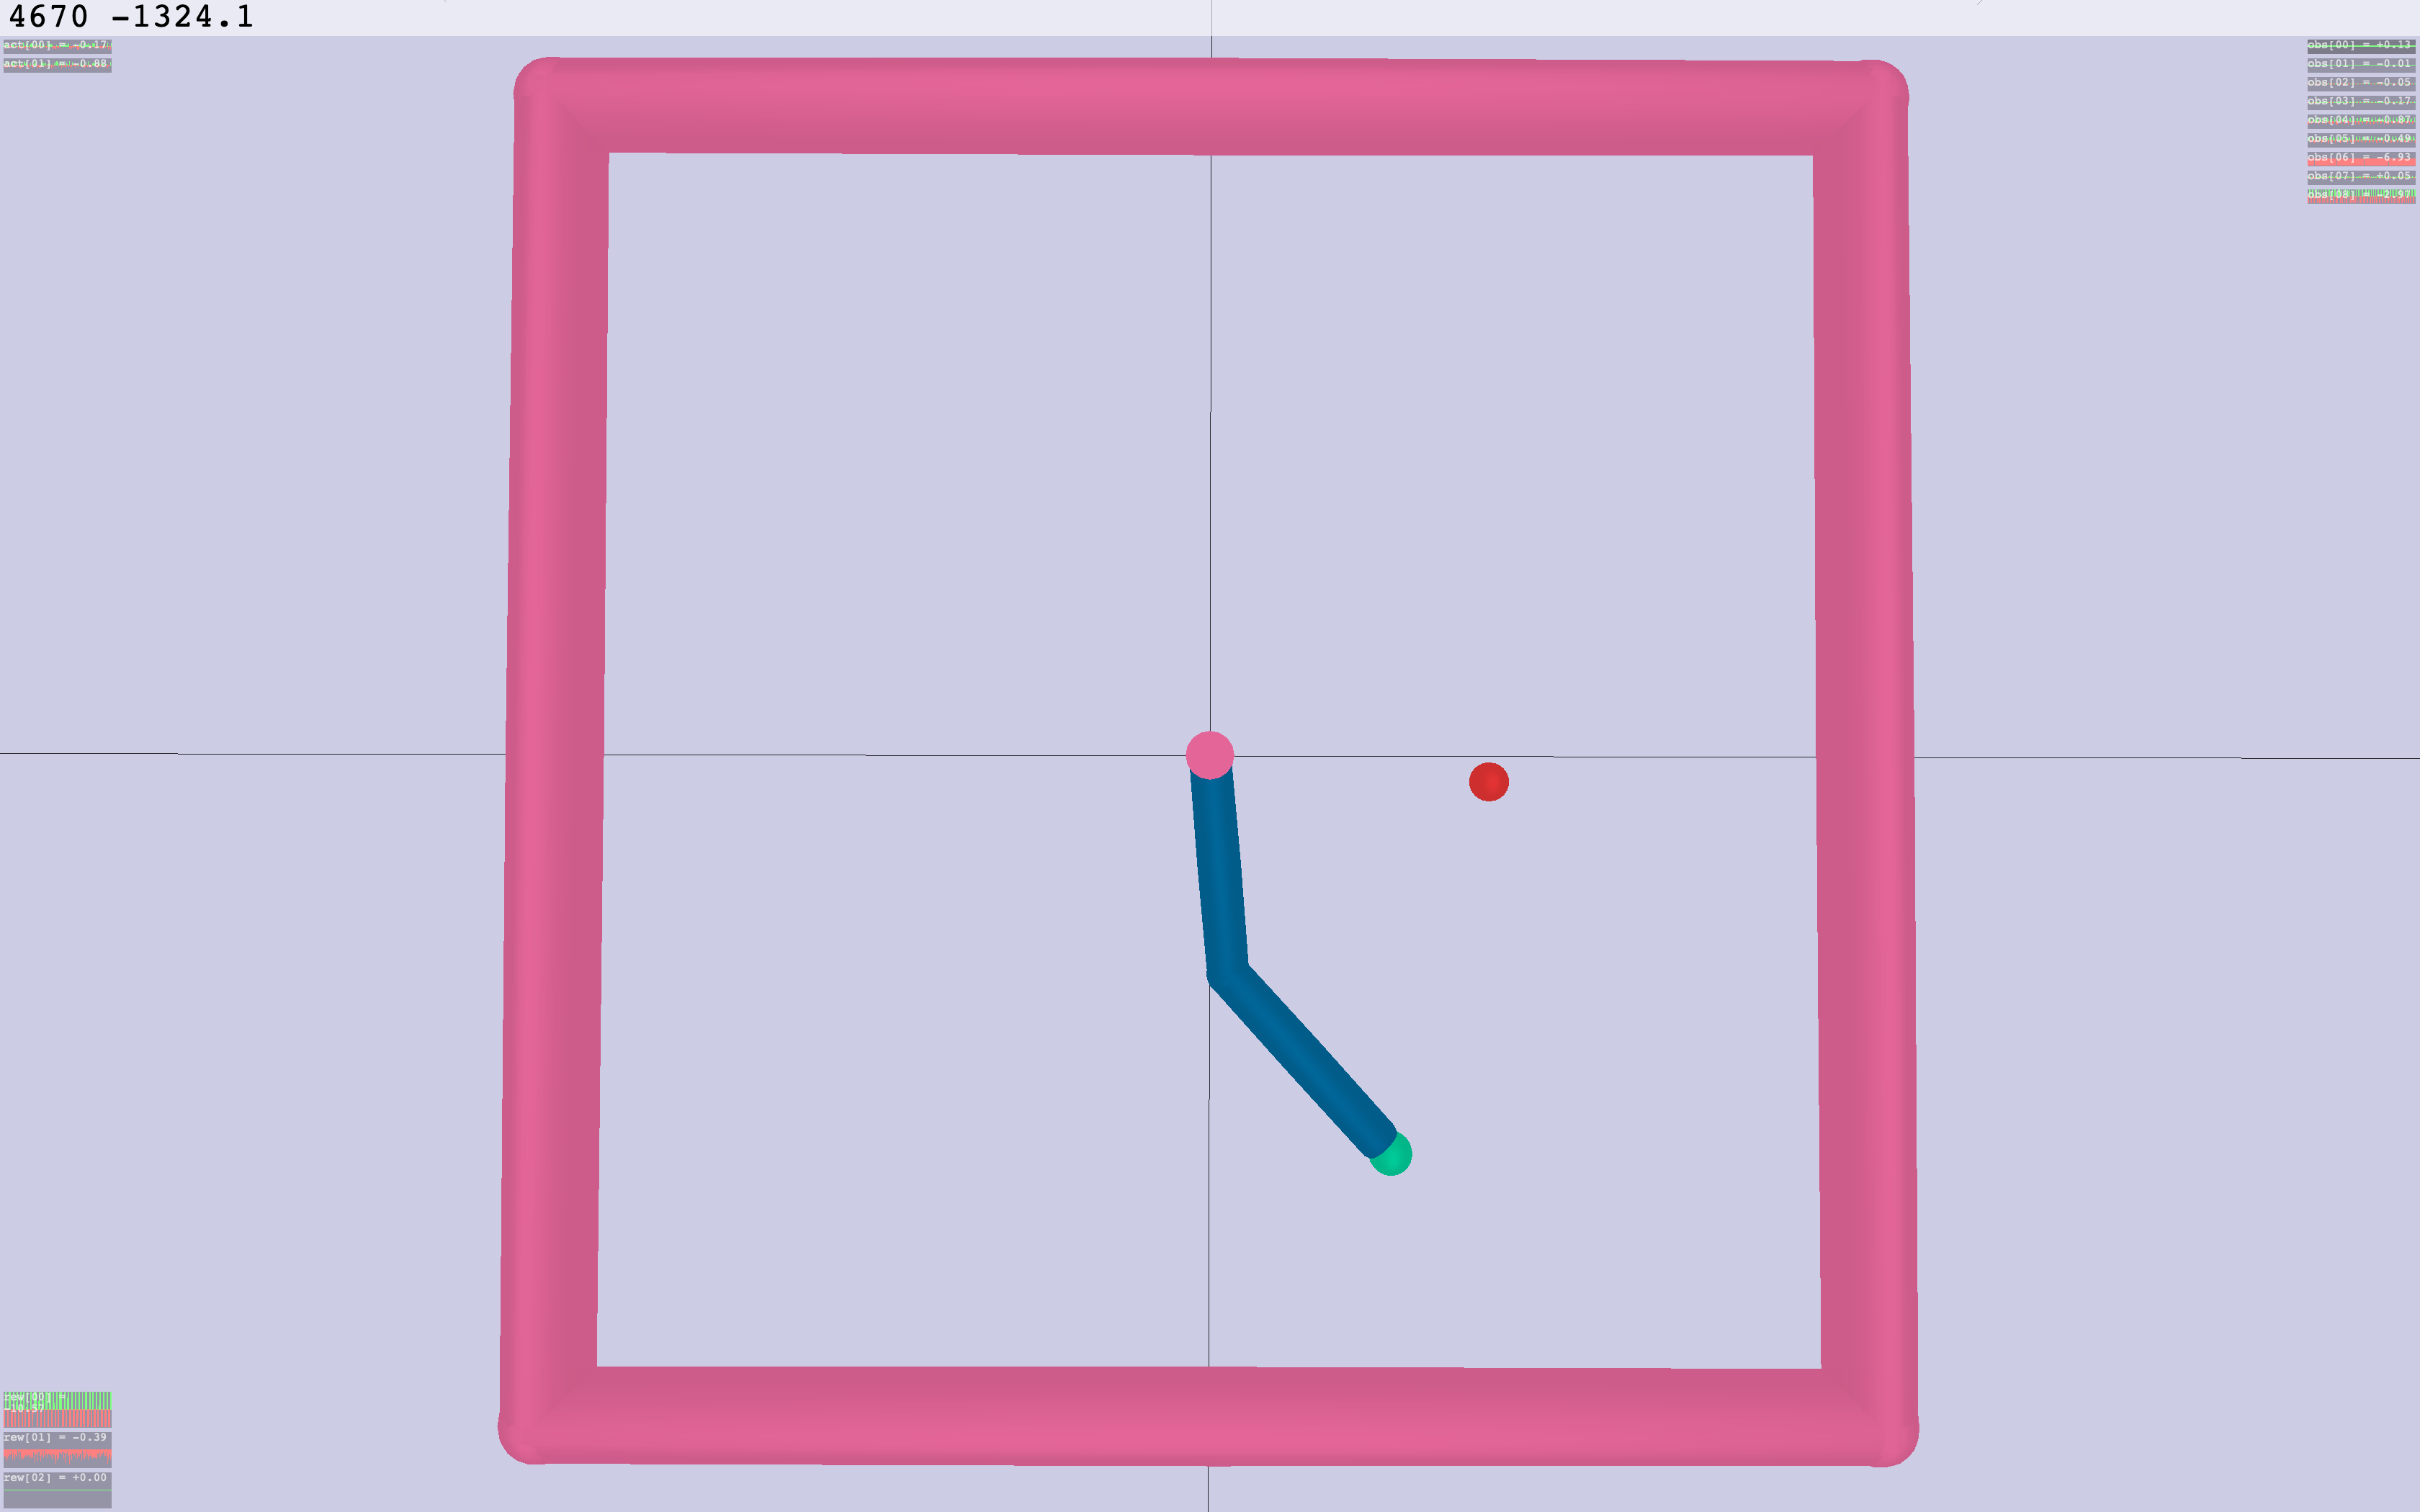
\includegraphics[width=0.7\linewidth]{figures/envs/openai_roboreacher.png}
            \caption{OpenAI Reacher Environment}
            \label{fig:openai_reacher}
    \end{center}
\end{figure}

\begin{table}[!htb]
    \centering
    \begin{subtable}{.4\linewidth}
        \centering
        \begin{tabular}{|c|c|}
        \hline
        \multicolumn{2}{|c|}{{\ul \textit{\textbf{Observation Space}}}}                                                                                   \\ \hline
        \multirow{2}{*}{\textbf{Target Position}}                                                                      & \textit{X Position}              \\ \cline{2-2} 
                                                                                                                    & \textit{Y Position}              \\ \hline
        \multirow{2}{*}{\textbf{Arm to Target Vector}}                                                                 & \textit{Position vector 0}       \\ \cline{2-2} 
                                                                                                                    & \textit{Position vector 1}       \\ \hline
        \multirow{2}{*}{\textbf{\begin{tabular}[c]{@{}c@{}}Current Relative Position\\ of Central Joint\end{tabular}}} & \textit{cosine of central joint} \\ \cline{2-2} 
                                                                                                                    & \textit{sine of central joint}   \\ \hline
        \multirow{2}{*}{\textbf{\begin{tabular}[c]{@{}c@{}}Current Relative Position\\ of Elbow Joint\end{tabular}}}   & \textit{cosine of elbow joint}   \\ \cline{2-2} 
                                                                                                                    & \textit{sine of elbow joint}     \\ \hline
        \end{tabular}
        \caption{Gym Reacher Observation Information}
        \label{tab:gym_reacher_obs}
    \end{subtable}%
    \hfill
    \begin{subtable}{.4\linewidth}
        \centering
        \begin{tabular}{|c|c|}
            \hline
            \multicolumn{2}{|c|}{{\ul \textit{\textbf{Action Space (Continuous)}}}}                             \\ \hline
            \multirow{2}{*}{\textbf{Center Joint Torque}} & \multirow{2}{*}{\textit{range(-1, 1)}} \\
                                                          &                                        \\ \hline
            \multirow{2}{*}{\textbf{Elbow Joint Torque}}  & \multirow{2}{*}{\textit{range(-1, 1)}} \\
                                                          &                                        \\ \hline
            \end{tabular}
            \caption{Gym Reacher Action Information}
            \label{tab:gym_reacher_actions}
    \end{subtable}%
    \caption{Gym Reacher Observation and Action Information}
\end{table}

the reward function is designed based on the distance between the arm and the target along with electricity cost of the torque and angular velocity of the arm with small epsilon amount in case of the joint is stuck. 

\clearpage

\textbf{Unity MLAgents: 2D and 3D Reacher Environment}

We have replicate the same openai gym reacher environment in unity to test the transferability between different physics engines, along with two 3d reacher environment (single and multi-agents) described below:

\textbf{Replicated Gym Env:}

\begin{figure}[H]
    \begin{center}
            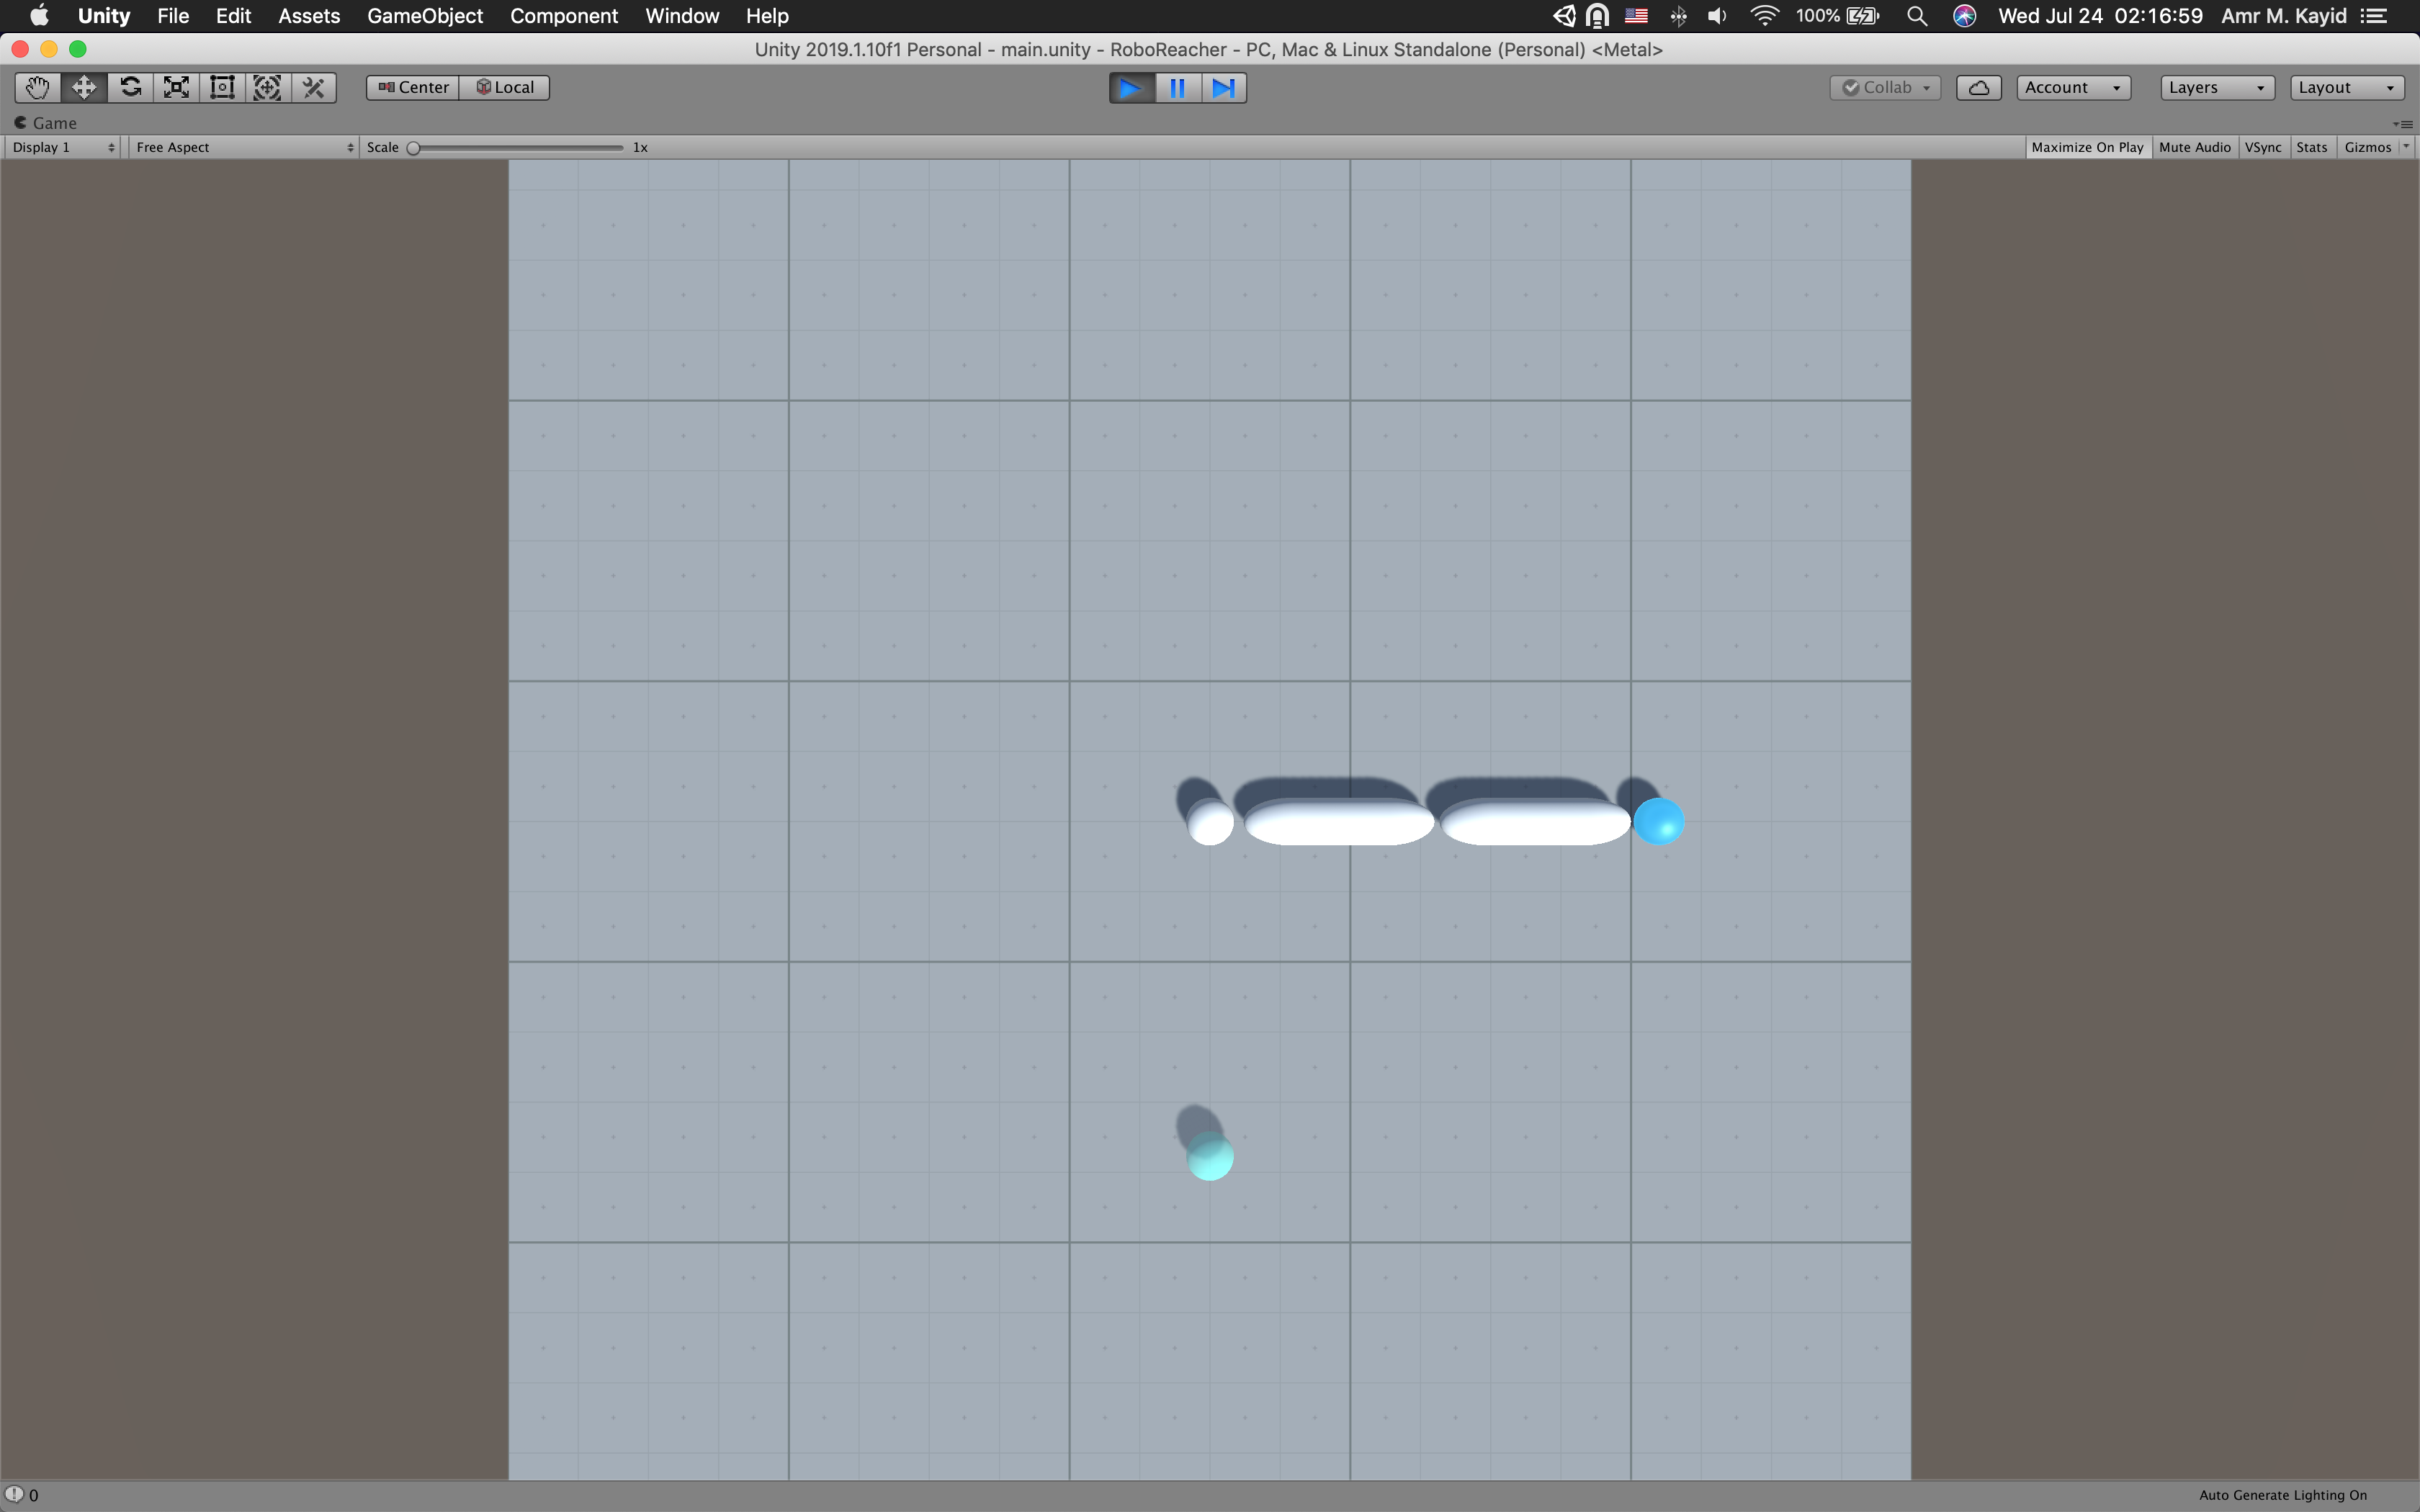
\includegraphics[width=0.7\linewidth]{figures/envs/unity_roboreacher.png}
            \caption{Replicated Gym Reacher Unity Environment}
            \label{fig:unity_reacher}
    \end{center}
\end{figure}


\textbf{Single Agent Reacher:} A robotic arm consist of two linked joints places in 3d plane surrounding it along with a moving sphere (target). The goal of the robotics arm it to reach target sphere and maintain following the point until the end of the episode. 

\begin{figure}[H]
    \begin{center}
            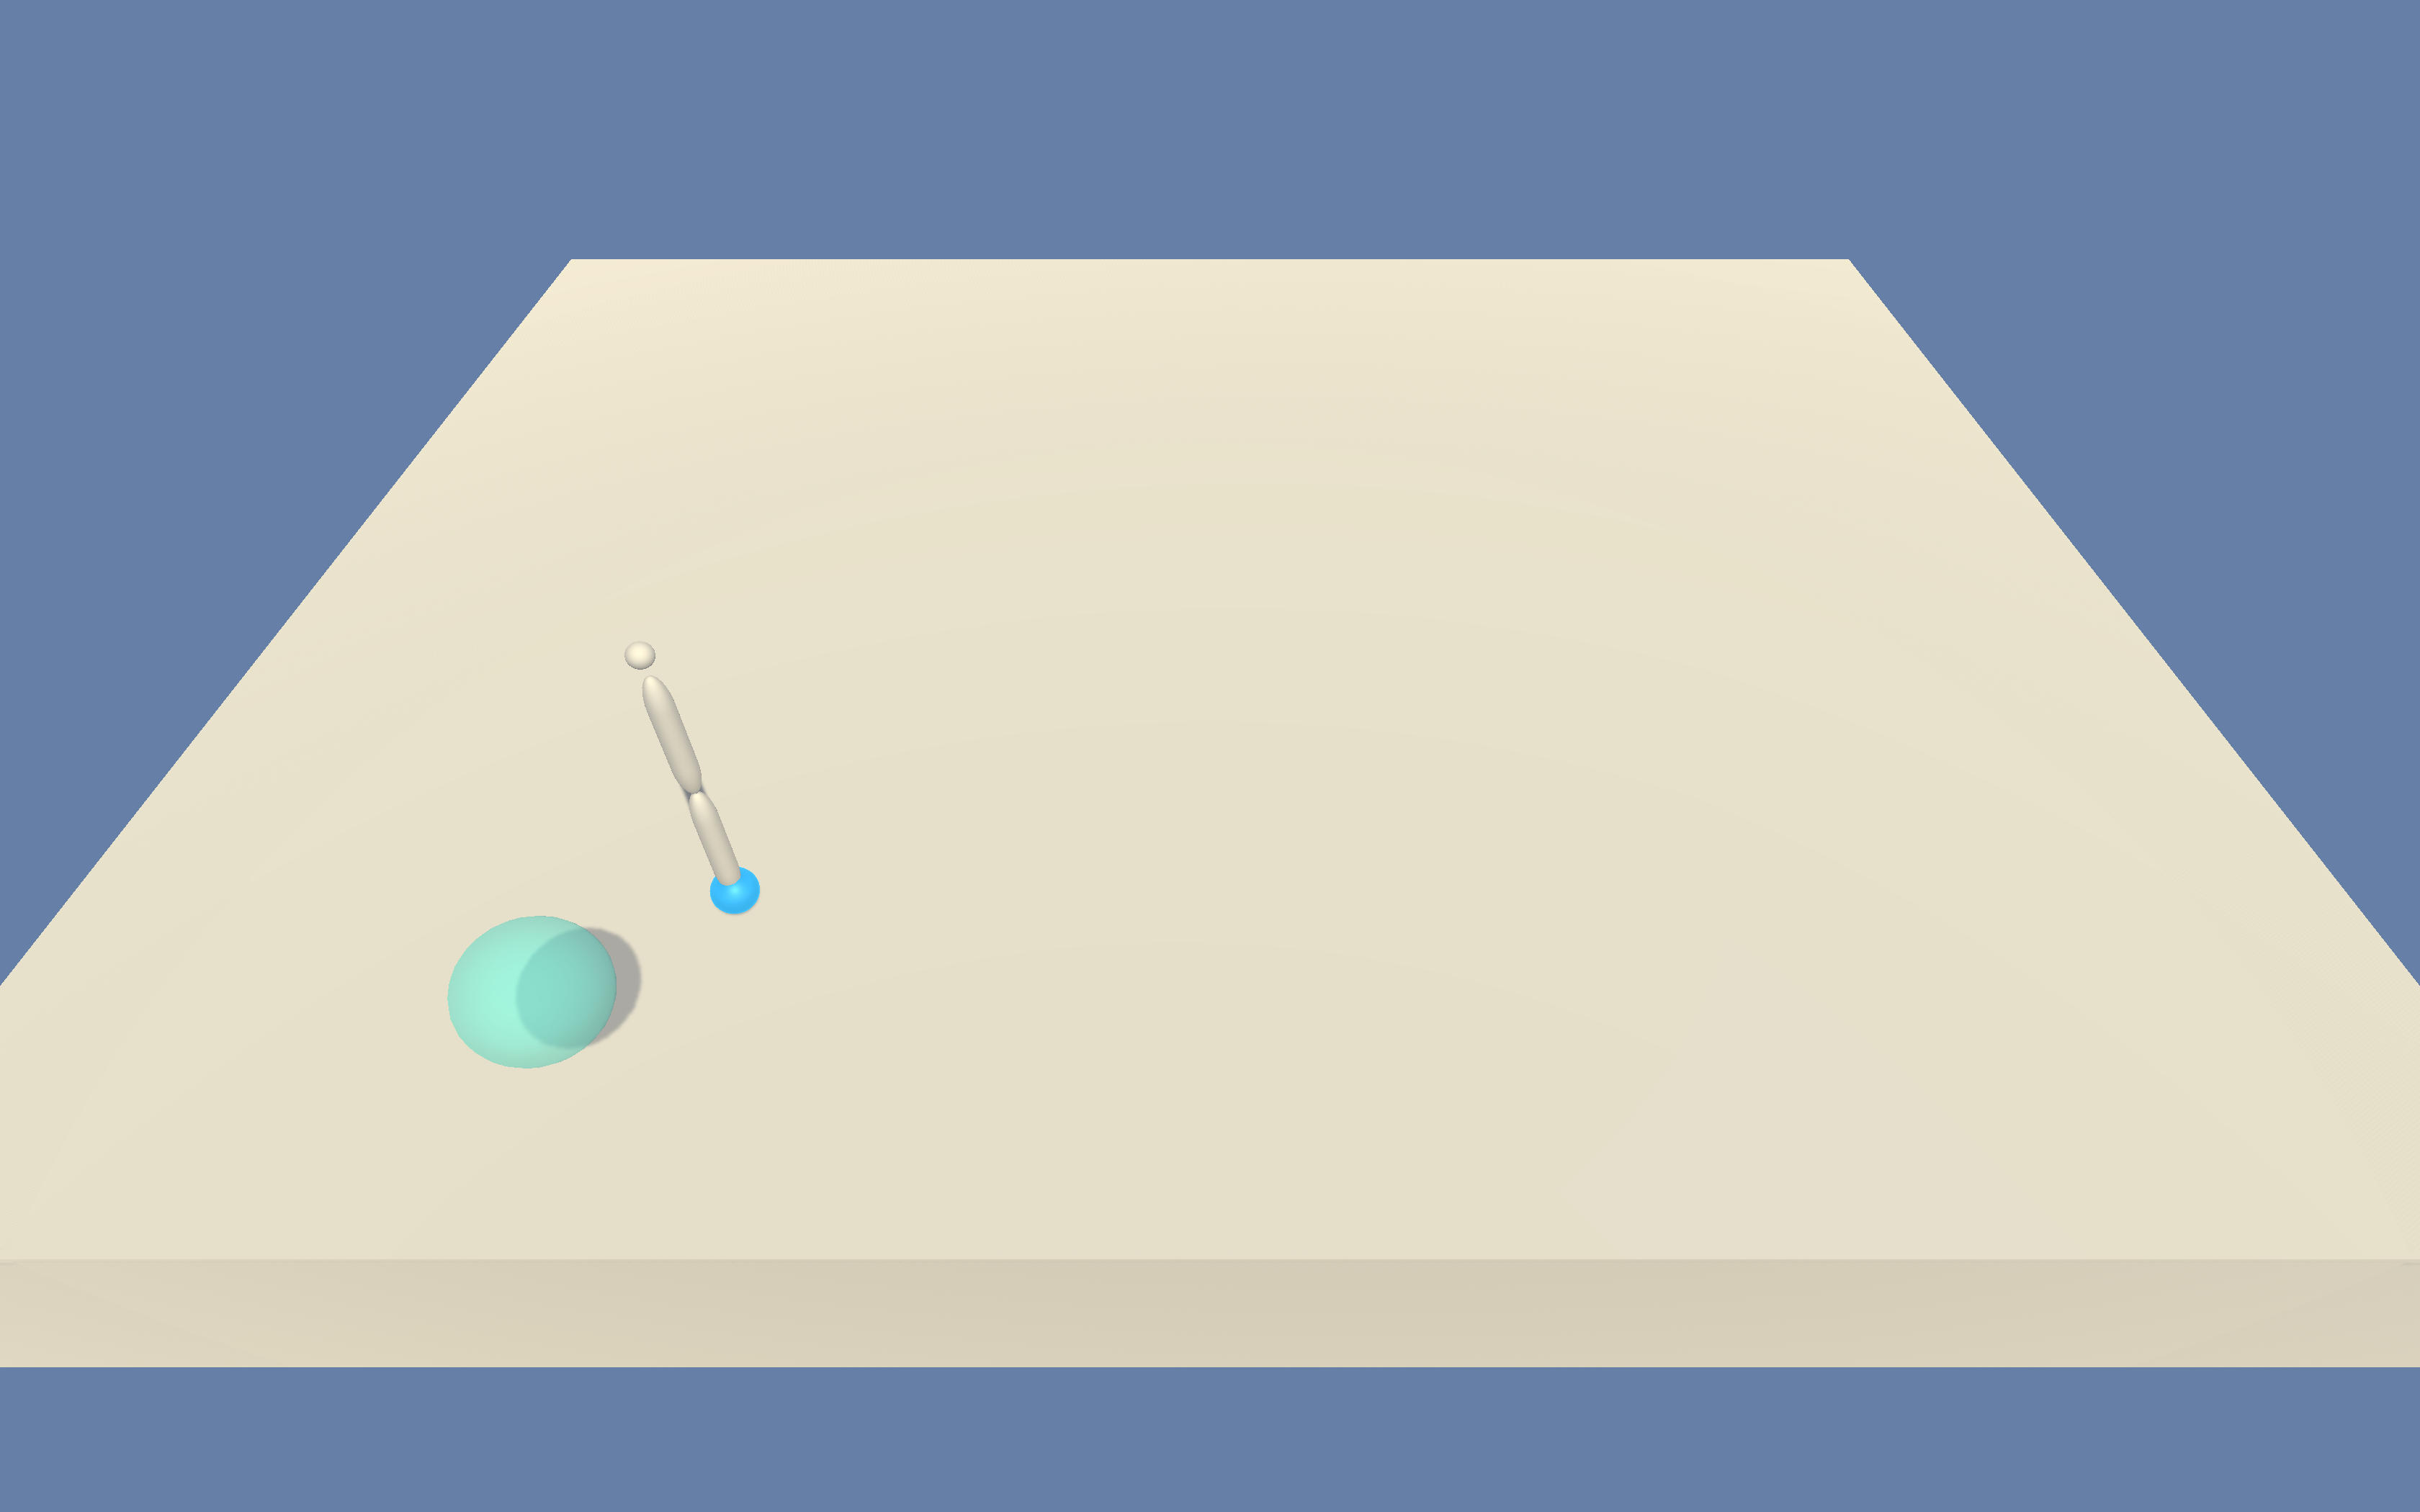
\includegraphics[width=0.7\linewidth]{figures/envs/unity_reacher_1.png}
            \caption{Unity Reacher Environment}
            \label{fig:unity_reacher_1}
    \end{center}
\end{figure}

\textbf{Multi-Agent Reacher:} in this environment, \textit{20 Agent} are used to parallelize the training process and collect more experiences and trajectories.

\begin{figure}[H]
    \begin{center}
            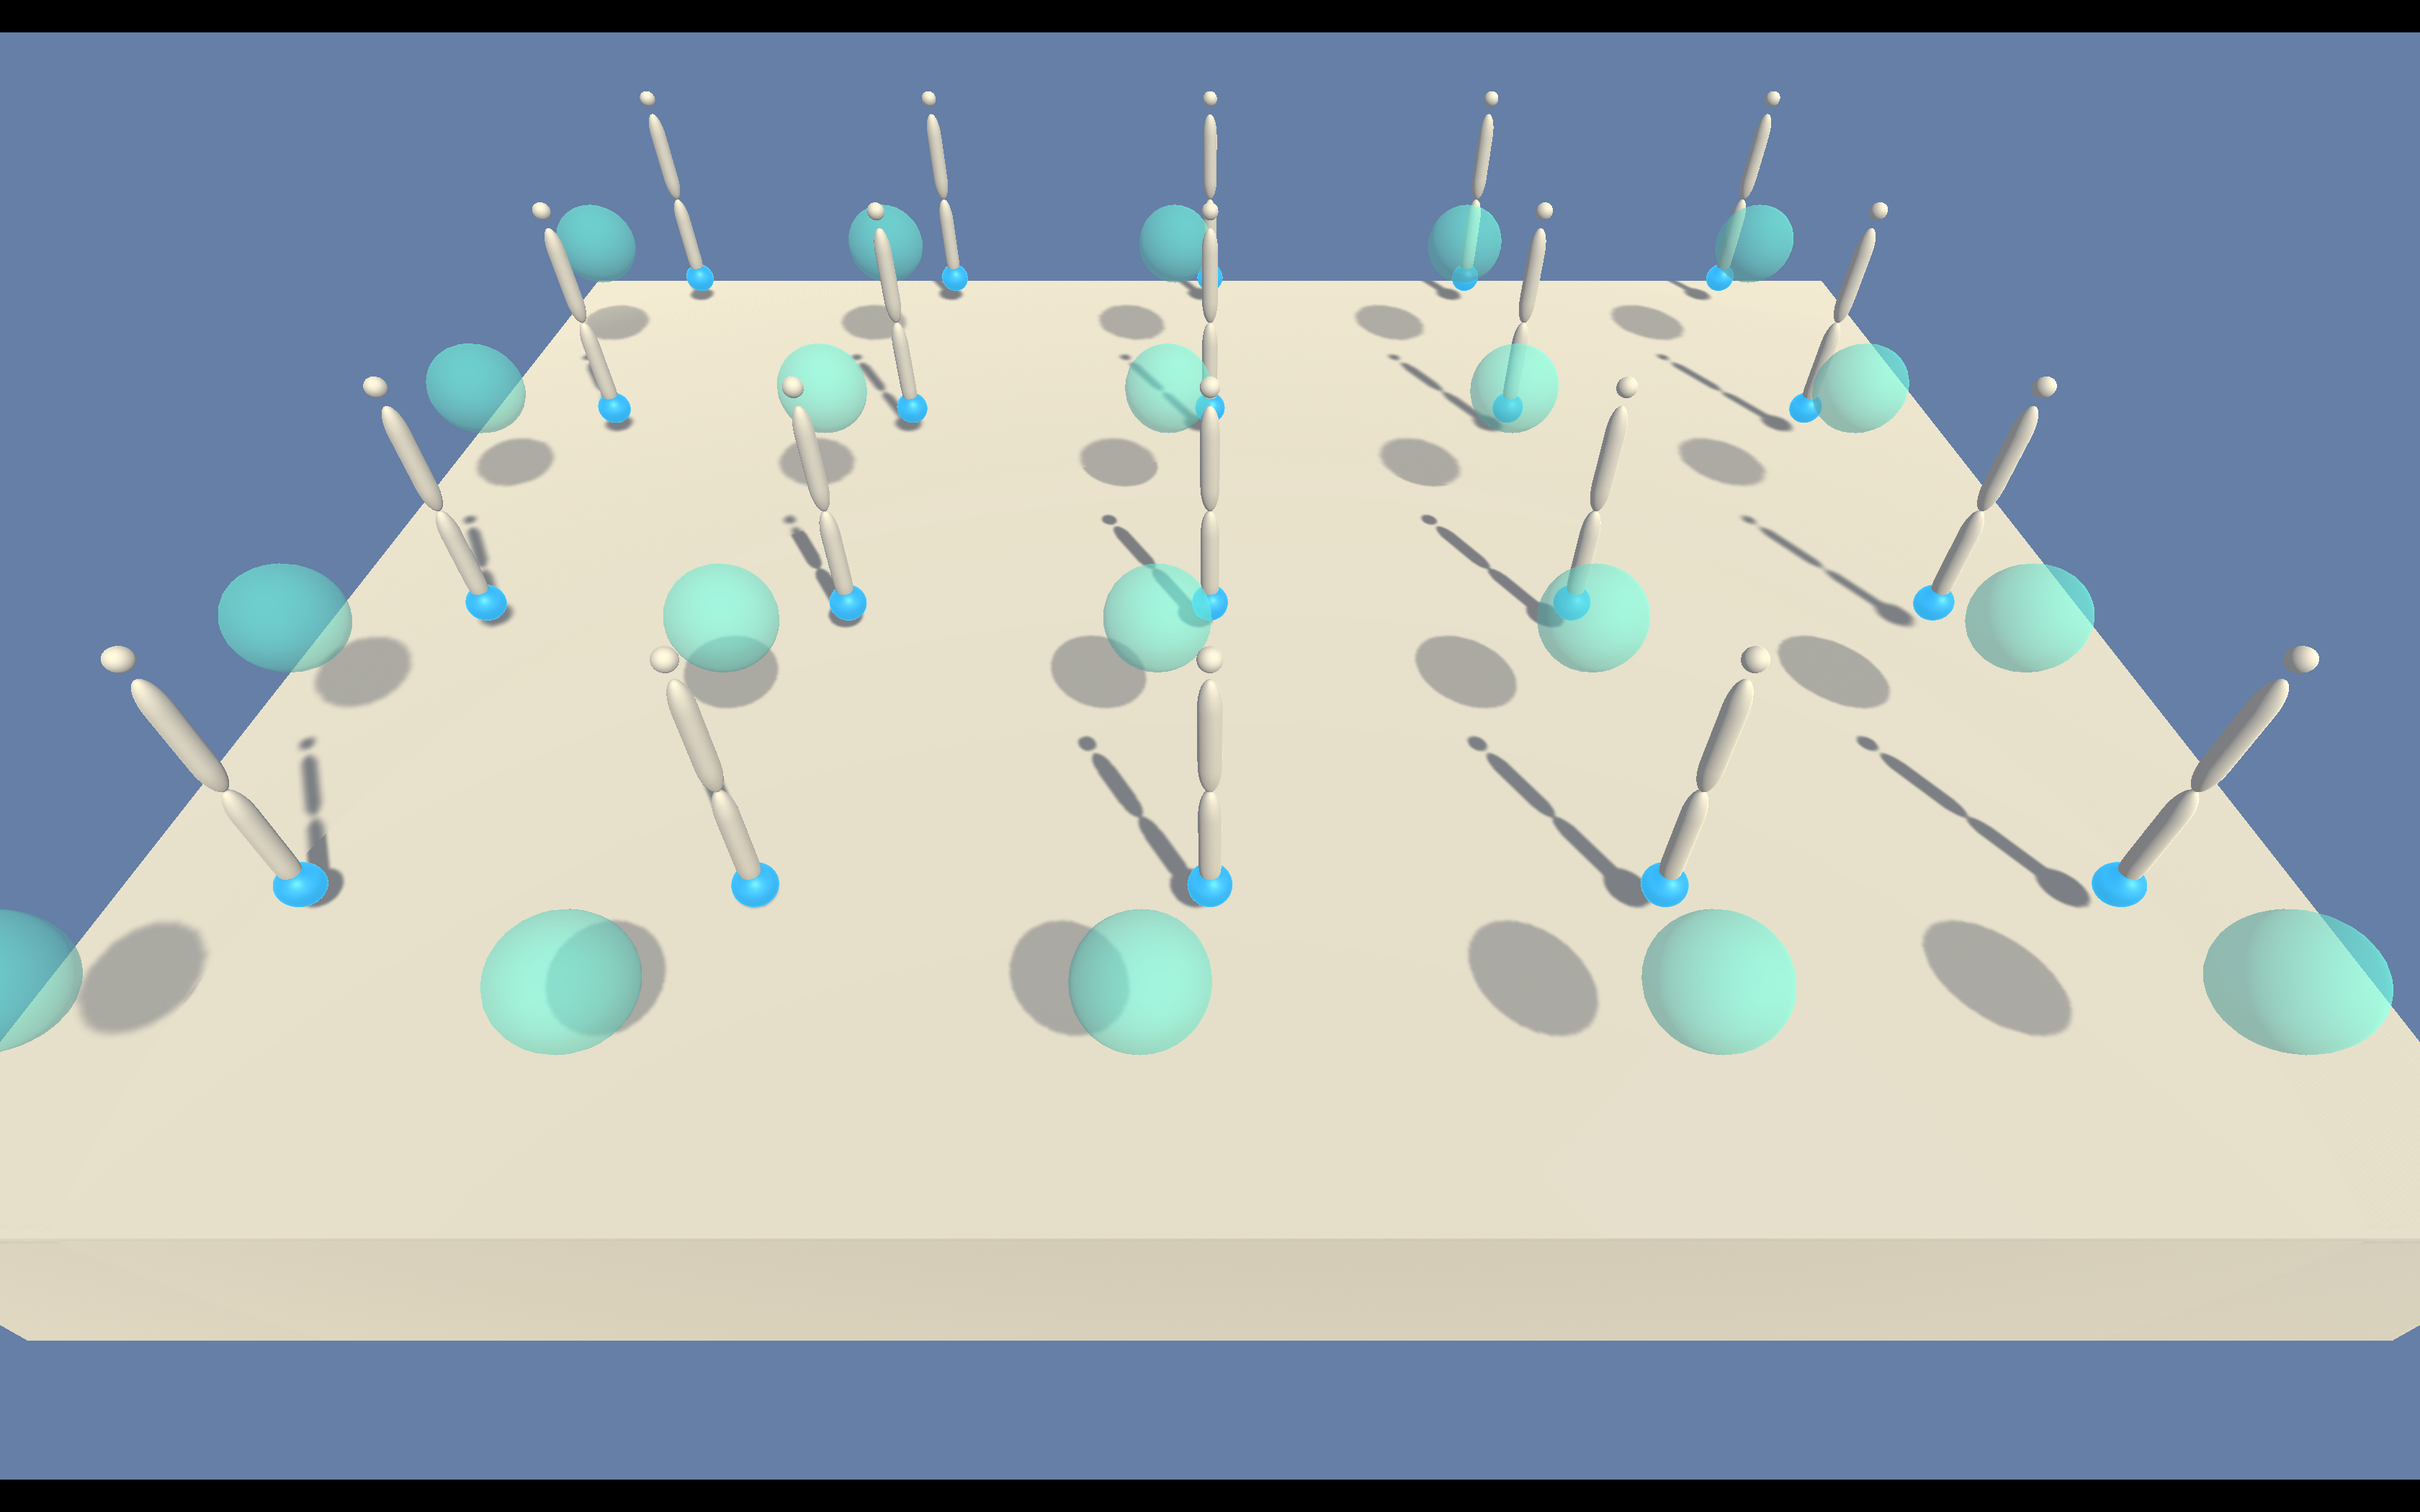
\includegraphics[width=0.7\linewidth]{figures/envs/unity_reacher_20.png}
            \caption{Unity Multi-Agent Reacher Environment}
            \label{fig:unity_reacher_20}
    \end{center}
\end{figure}

% !TeX root = ../../main.tex
% Add the above to each chapter to make compiling the PDF easier in some editors.

\chapter{Setup and Implementation}\label{chapter:setup_and_implementation}

In this chapter, the full details of the setups will be introduced. First, the used software framework will be presented. Then, our environments architecture and integration with the framework will be explained. Then, a brief description for the agents and algorithms will be shown. Lastly, description for all the used environments in our experiments will be provided.

\section{Overview}

Our approach is to setup a distributed learning architecture to run multiple experiments between selected environment and compare the results between training in normal non-distributed and distributed modes. We selected relatively close environment to robotics simulation with continuous observation and action spaces. A new abstract classes is introduced to run with the selected framework and unify the differences between different environments and physics simulators. A selection of the state of the art algorithms is used to train our reinforcement learning agents and compare between the algorithm and the modes for each algorithm.

\section{Software}
\textbf{Ray Framework~\parencite{moritz2018ray}: } Ray is a fast and simple framework for building and running distributed applications. The same code can be run on a single machine to achieve efficient multiprocessing, and it can be used on a cluster for large computations. Ray provide high scalability and a unified API for a variety of applications which is very useful for our experiments. Ray executes tasks asynchronously to achieve parallelism enabling us to run multiple environments in the same experiment to benefit from collection more experiences and trajectories for the agent.

\textbf{OpenAI Gym~\parencite{brockman2016openai}: } openai gym is a toolkit for developing and comparing reinforcement learning algorithms. It supports teaching agents everything from walking to playing games like Pong or Pinball. It has an open source interface to reinforcement learning tasks which provides an easy-to-use suite of reinforcement learning tasks. 

The core gym interface is \textbf{Env}, which is the unified environment interface. 
The following are the methods for the abstracted gym Env:

\begin{itemize}
    \item \textit{\textbf{\colorbox{gray!20}{reset(self)}}}: Reset the environment's state. Returns observation.
    \item \textit{\textbf{\colorbox{gray!20}{step(self, action)}}}: Step the environment by one time-step. Returns observation, reward, done, info.
    \item \textit{\textbf{\colorbox{gray!20}{render(self, mode='human')}}}: Render one frame of the environment. The default mode will do something human friendly, such as pop up a window.
\end{itemize}

\textbf{Unity MLAgents~\parencite{juliani2018unity}: } unity mlagents toolkit is an open-source Unity plugin that enables games and simulations to serve as environments for training intelligent agents. It has more realistic and complex simulation environments. It provides the ability to flexibly configure
the simulation. By taking advantage of Unity as a simulation platform, the toolkit enables the development of learning environments which are rich in sensory and physical complexity, provide compelling cognitive challenges, and support dynamic multi-agent interaction. Agents can be trained using reinforcement learning, imitation learning, neuroevolution, or other machine learning methods through a simple-to-use Python API. They provide implementations of state-of-the-art algorithms to enable game developers and hobbyists to easily train intelligent agents for 2D, 3D and VR/AR games. We are using this to test running multiple agents in the same environment and compare the effect with one agent only. Also, to experiment the transferability between different physics simulators.

\section{Architecture}

At a high level, ray provides an \textbf{\colorbox{gray!20}{Trainer}} class which holds a policy for environment interaction. Through the trainer interface~\ref{fig:ray_trainer}, the policy can be trained, check-pointed, or an action computed. In multi-agent training, the trainer manages the querying and optimization of multiple policies at once. It provides custom resources configurations~\ref{fig:ray_config}, which can control the degree of parallelism used by setting the \colorbox{gray!20}{\texttt{num\_workers}} hyper-parameter for most algorithms. The number of GPUs the driver should use can be set via the \colorbox{gray!20}{\texttt{num\_gpus}} option. Similarly, the resource allocation to workers can be controlled via \colorbox{gray!20}{\texttt{num\_cpus\_per\_worker}}, \colorbox{gray!20}{\texttt{num\_gpus\_per\_worker}}, and \colorbox{gray!20}{\texttt{custom\_resources\_per\_worker}}. The number of GPUs can be a fractional quantity to allocate only a fraction of a GPU. For example, with DQN you can pack five trainers onto one GPU by setting \colorbox{gray!20}{\texttt{num\_gpus}: 0.2}.

\begin{figure}[H]
	\centering
	\begin{subfigure}[b]{0.4\textwidth}
		\centering
		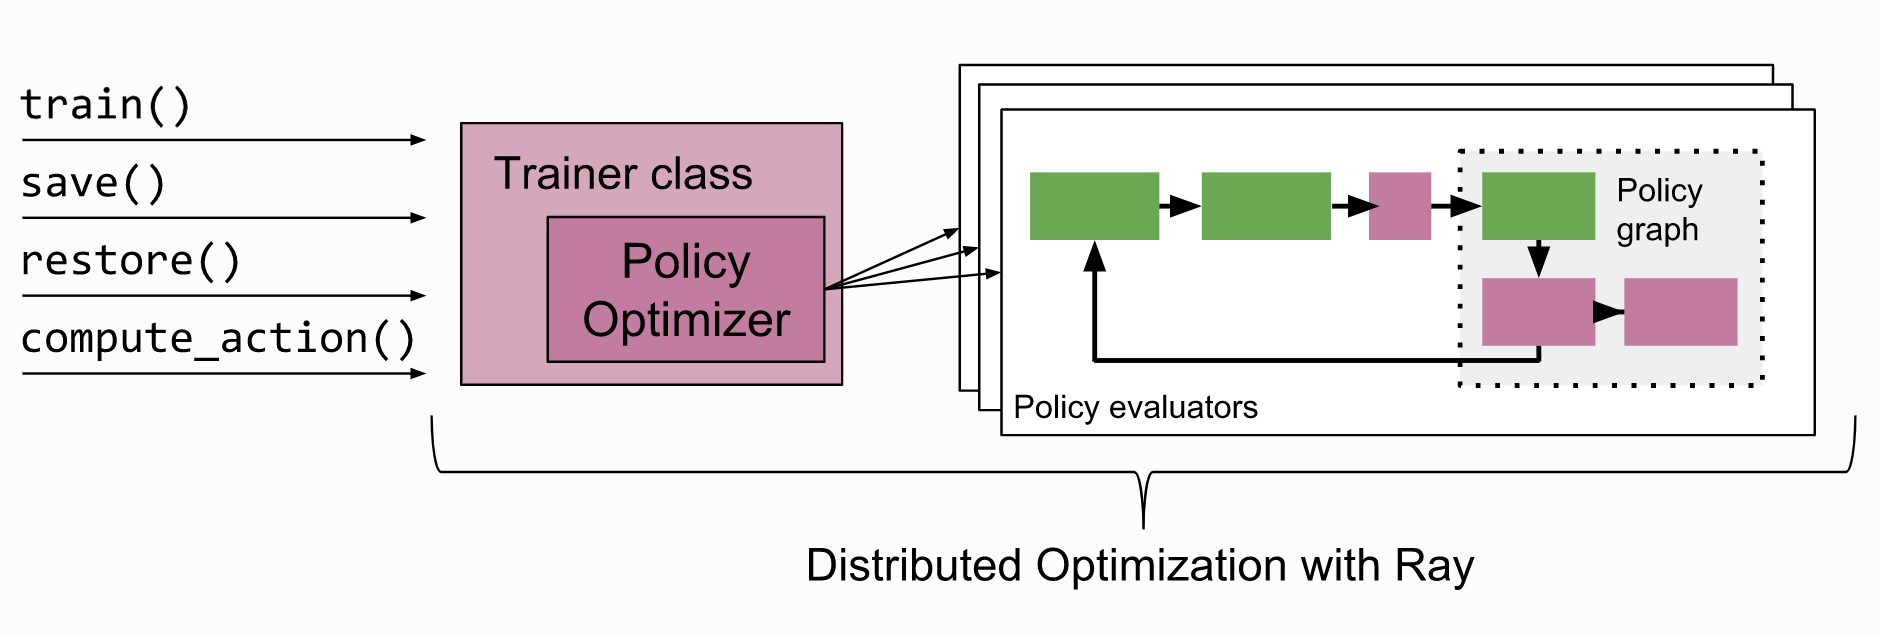
\includegraphics[width=\textwidth]{figures/architecture/ray_trainer.png}
		\caption{Ray Training Process}
		\label{fig:ray_trainer}
    \end{subfigure}
    \hfill
	\begin{subfigure}[b]{0.4\textwidth}
		\centering
		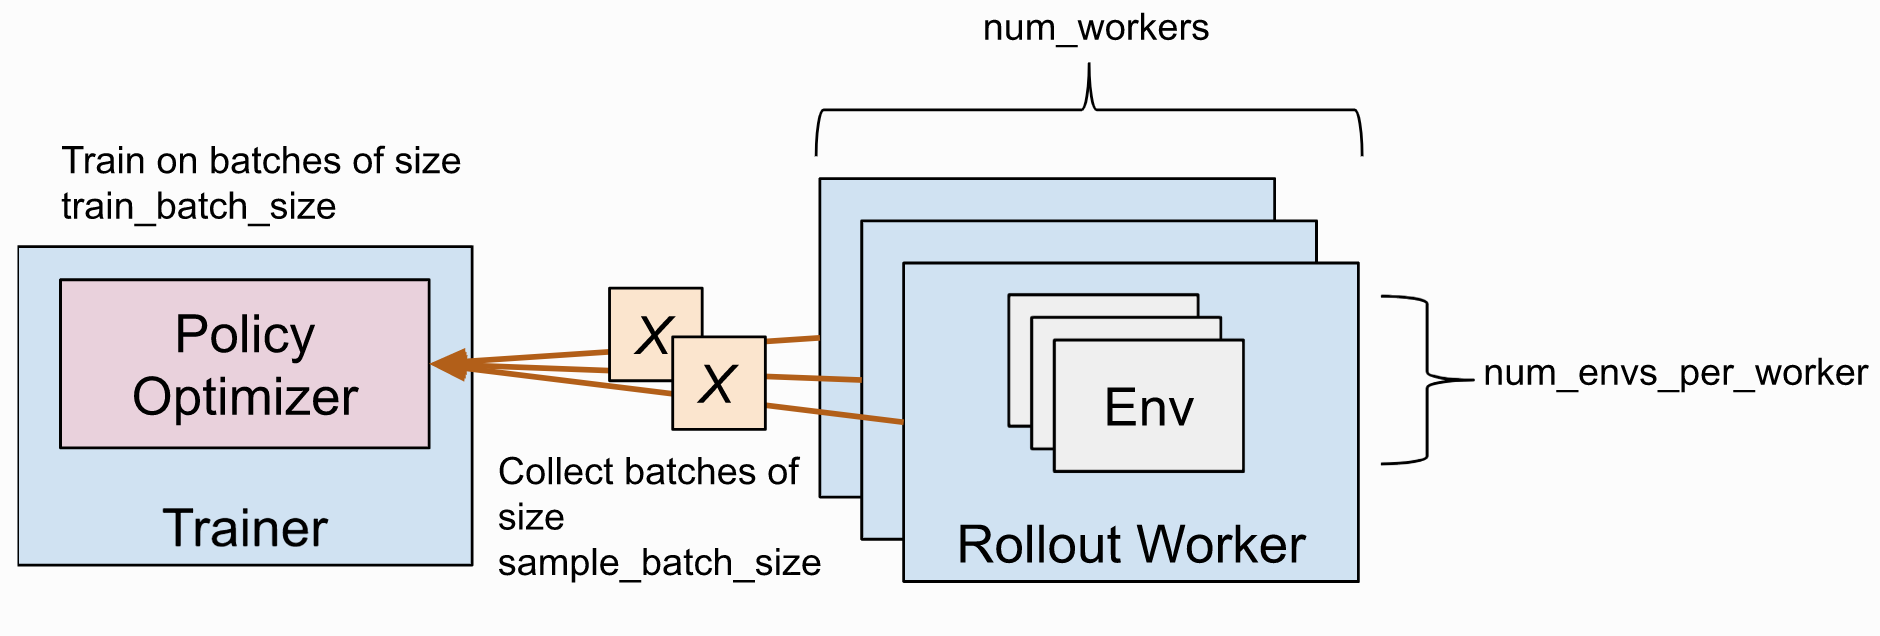
\includegraphics[width=\textwidth]{figures/architecture/ray_config.png}
        \caption{Ray Configurable resources}
		\label{fig:ray_config}
	\end{subfigure}
	\hfill
	   \caption{General Overview of Ray framework~\parencite{moritz2018ray}}
	   \label{fig:ray}
\end{figure}

Since ray support only OpenAI Gym environments along with their provided multi-agent and also batched environments, we had to implement our custom environment to unify between unity mlagents and openai gym environments. Also, we implemented our custom Multi-Agent environments for both used environments as shown in the following figure~\ref{fig:ray_envs}.

\begin{figure}[H]
	\centering
		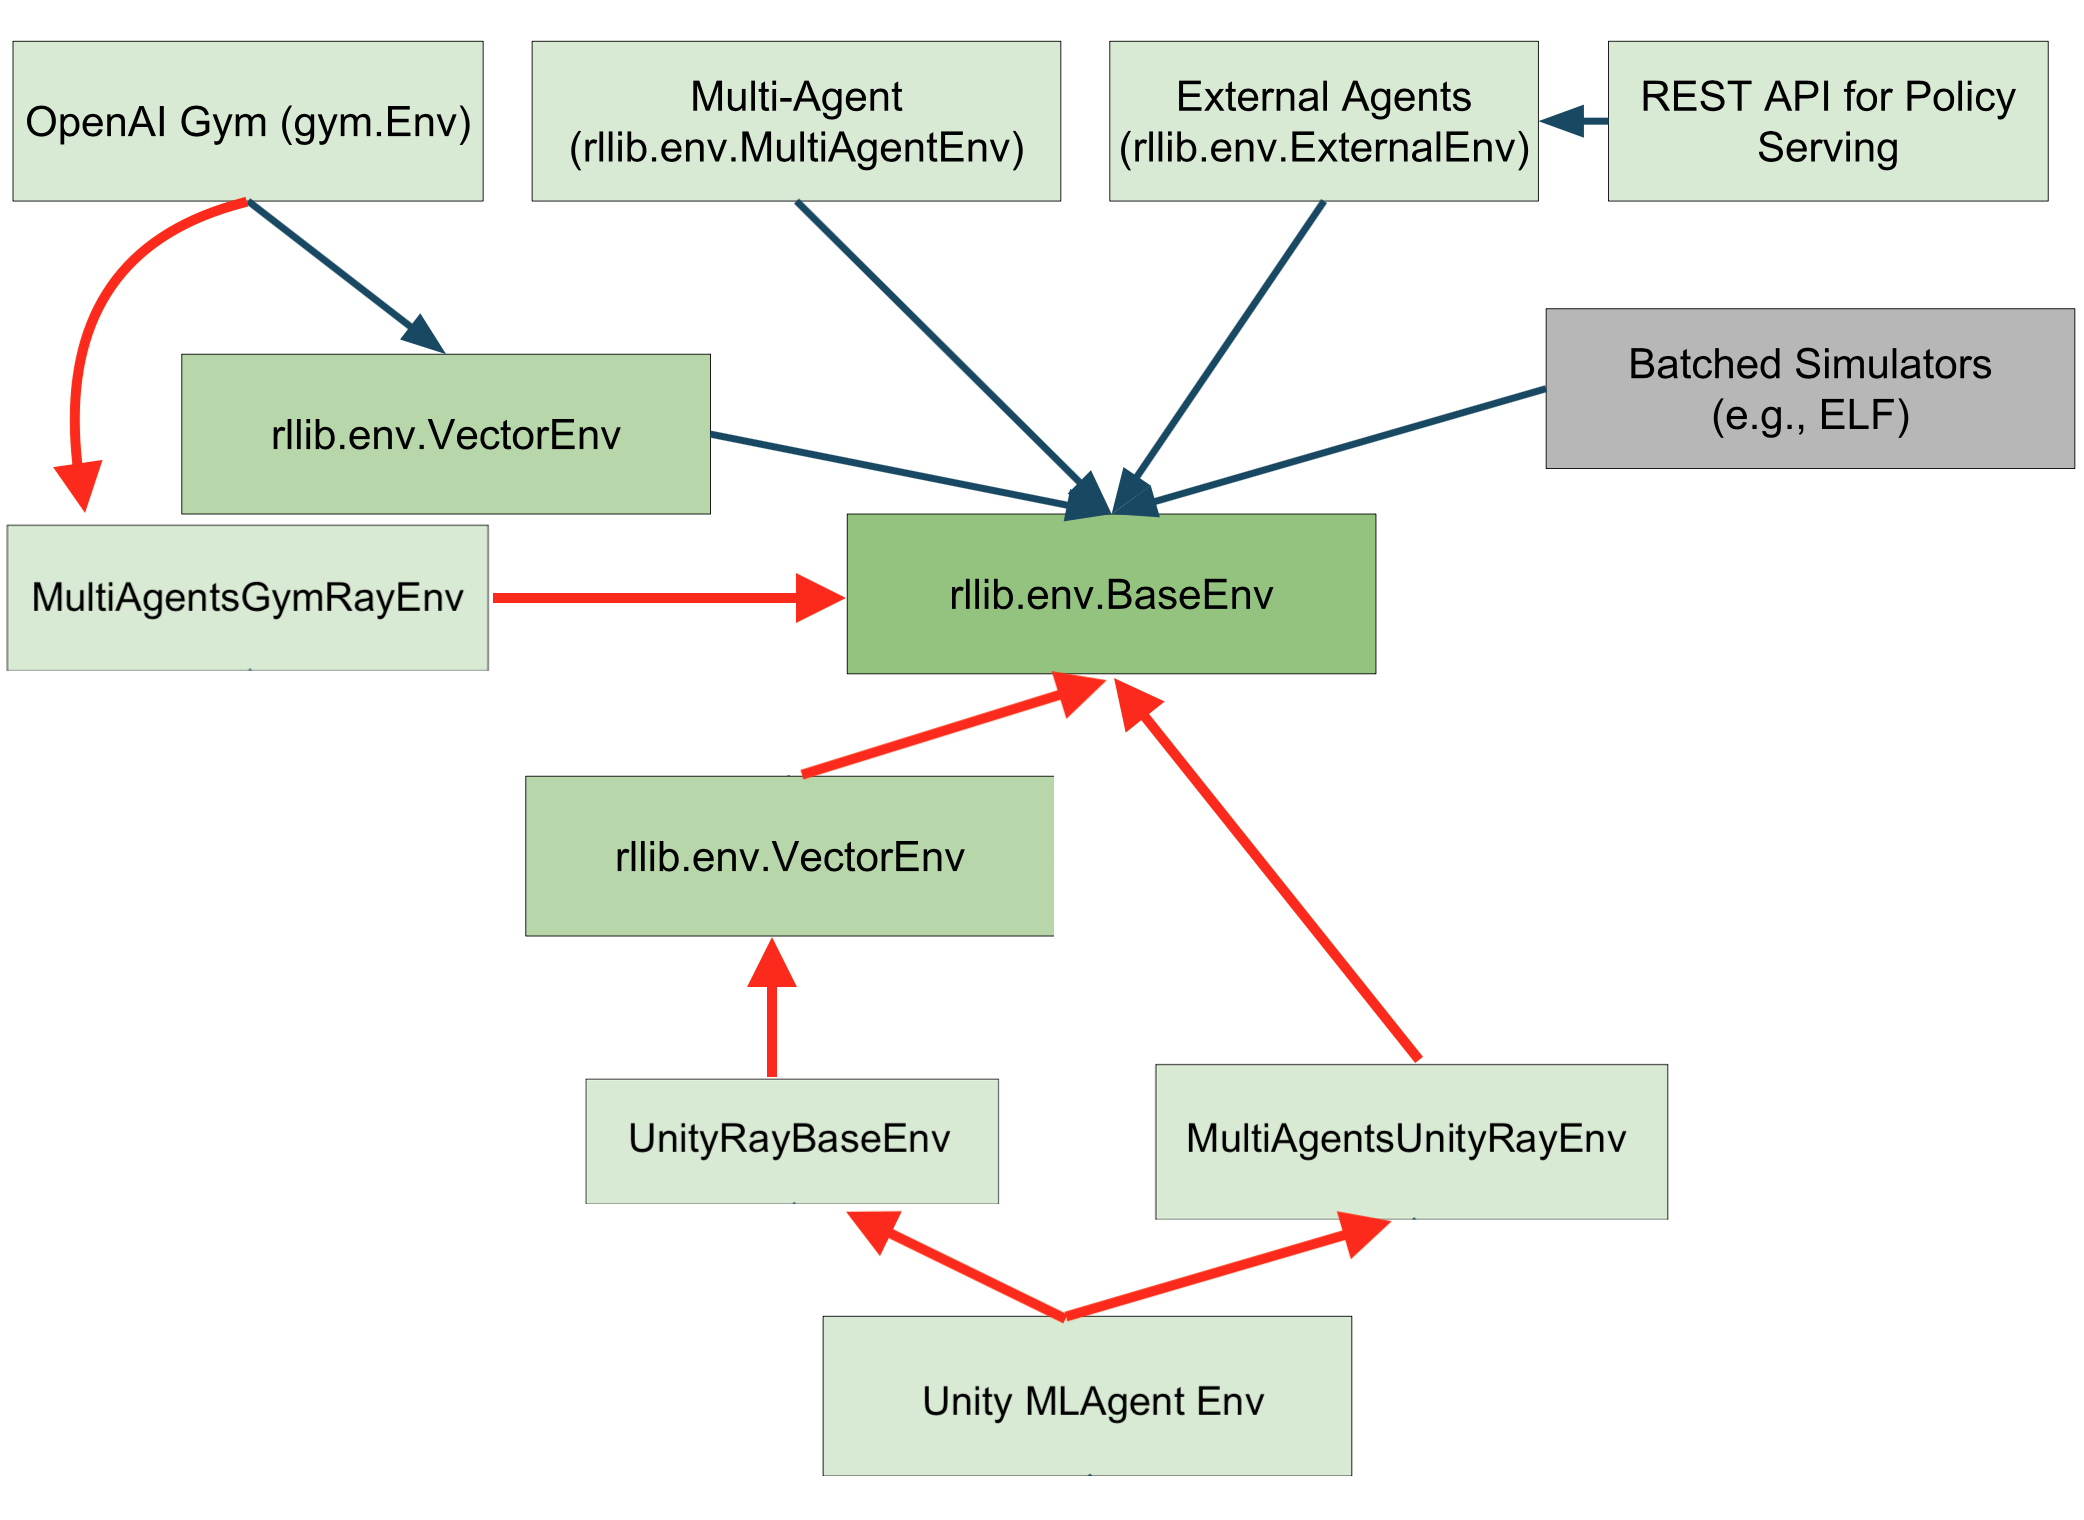
\includegraphics[width=\linewidth]{figures/architecture/ray_envs.png}
		\caption{Our Custom Environments}
		\label{fig:ray_envs}
\end{figure}

\clearpage

Custom environments implementations and methods are described below:

\textbf{UnityRayEnv}:\\
our base unity environment maps the observations and actions from unity mlagents toolkit to be compatible with Ray BaseEnv. Since unity mlagents deals with brains that control the agents and the environments we had to convert it to the required \colorbox{gray!20}{\texttt{observation\_space}} and \colorbox{gray!20}{\texttt{action\_space}} for ray env with the following methods:
\begin{itemize}
    \item \textit{\textbf{\colorbox{gray!20}{\texttt{\_\_init\_\_(self)}}}}: Create the unity environment from the unity build env, convert the observation and action spaces to be ray-compatible.
    \item \textit{\textbf{\colorbox{gray!20}{reset(self)}}}: Reset the environment's state. Returns observation.
    \item \textit{\textbf{\colorbox{gray!20}{step(self, action)}}}: Step the environment by one time-step. Returns observation, reward, done, info.
\end{itemize}

\textbf{MultiAgentsUnityRayEnv}:\\
this class inherit from both \colorbox{gray!20}{\textbf{UnityRayEnv}} and \colorbox{gray!20}{\textbf{MultiAgentEnv}}~\ref{fig:ray_multiagentenv}. The difference from the base environment is in both methods \textit{\textbf{\colorbox{gray!20}{reset(self)}}} and \textit{\textbf{\colorbox{gray!20}{step(self, \texttt{actions\_dict})}}}, where the reset function reset all the observations for each agent that exist in the environment and step function take a dictionary of actions corresponding for each action of a single agent. The same applies to \textbf{MultiAgentsGymRayEnv}.

\begin{figure}[H]
	\centering
		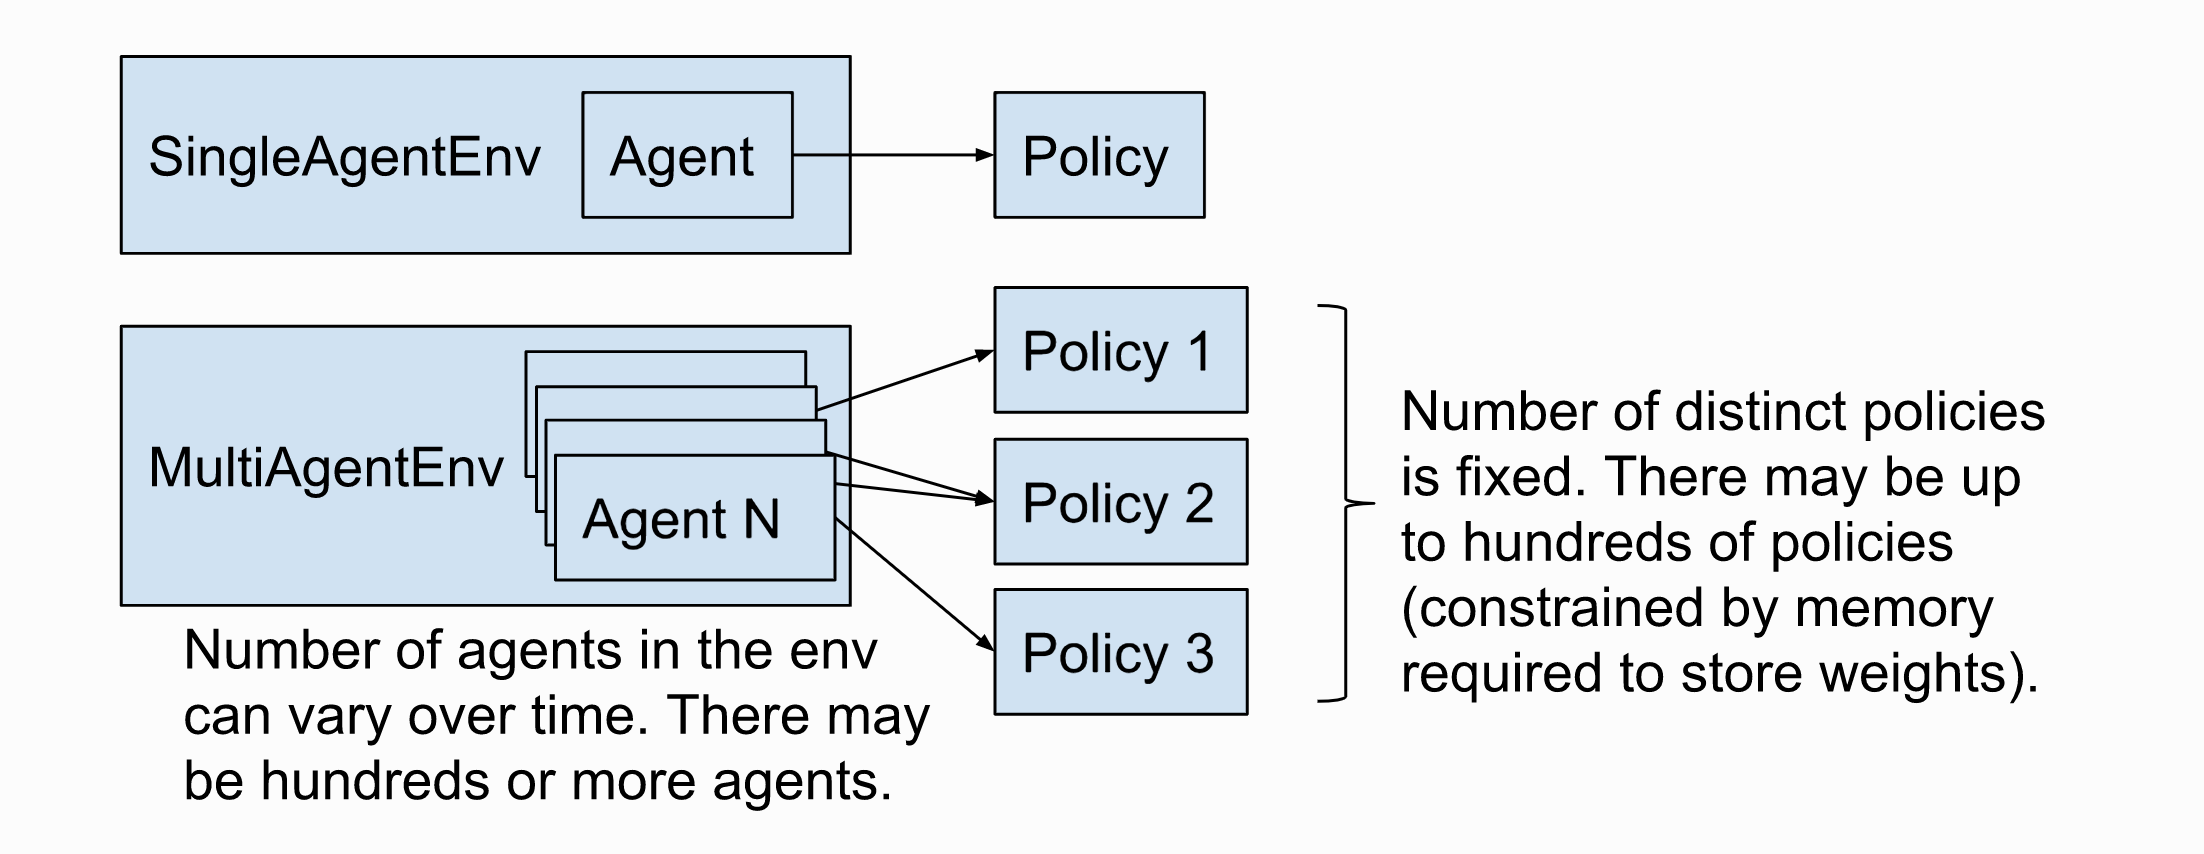
\includegraphics[width=\linewidth]{figures/architecture/ray_multiagentenv.png}
		\caption{Ray MultiAgentEnv}
		\label{fig:ray_multiagentenv}
\end{figure}

\section{Agents and Algorithms}

\begin{itemize}
    \item \textbf{Proximal Policy Optimization (PPO)}: PPO’s clipped objective supports multiple SGD passes over the same batch of experiences. RLlib’s multi-GPU optimizer pins that data in GPU memory to avoid unnecessary transfers from host memory, substantially improving performance over a naive implementation. RLlib’s PPO scales out using multiple workers for experience collection, and also with multiple GPUs for SGD.

    \item \textbf{Distributed Prioritized Experience Replay (Ape-X)}: Ape-X variations of DQN, DDPG, use a single GPU learner and many CPU workers for experience collection. Experience collection can scale to hundreds of CPU workers due to the distributed prioritization of experience prior to storage in replay buffers.

    \item \textbf{Importance Weighted Actor-Learner Architecture (IMPALA)}: In IMPALA, a central learner runs SGD in a tight loop while asynchronously pulling sample batches from many actor processes. RLlib’s IMPALA implementation uses DeepMind’s reference V-trace code. Note that we do not provide a deep residual network out of the box, but one can be plugged in as a custom model. Multiple learner GPUs and experience replay are also supported.
\end{itemize}

\section{Environments and Tasks Description}
Our task is robotic related task, where we have a robotic arm consist of two linked joints \textit{(agent)} and moving sphere \textit{(target)}. The robotic arm and the goal differ according to the environment used. We have a one experiment where is the agent movement is in 2D and the goal of the agent it to reach the target as fast as possible to maximize the given cumulative reward. In the second experiment, the agent can move in 3D and the goal is to keep track of the moving target and move with it along the 3D space.

Following is detailed description for all the environment used in our experiments.

\textbf{OpenAI: Reacher Environment}

Our first and baseline environment is \textit{Reacher Environment}~\ref{fig:openai_reacher}: A robotic arm consist of two linked joints places in a squared arena surrounding it along with a moving sphere (target). The goal of the robotics arm it to reach target sphere and maintain following the point until the end of the episode. 

\begin{figure}[H]
    \begin{center}
            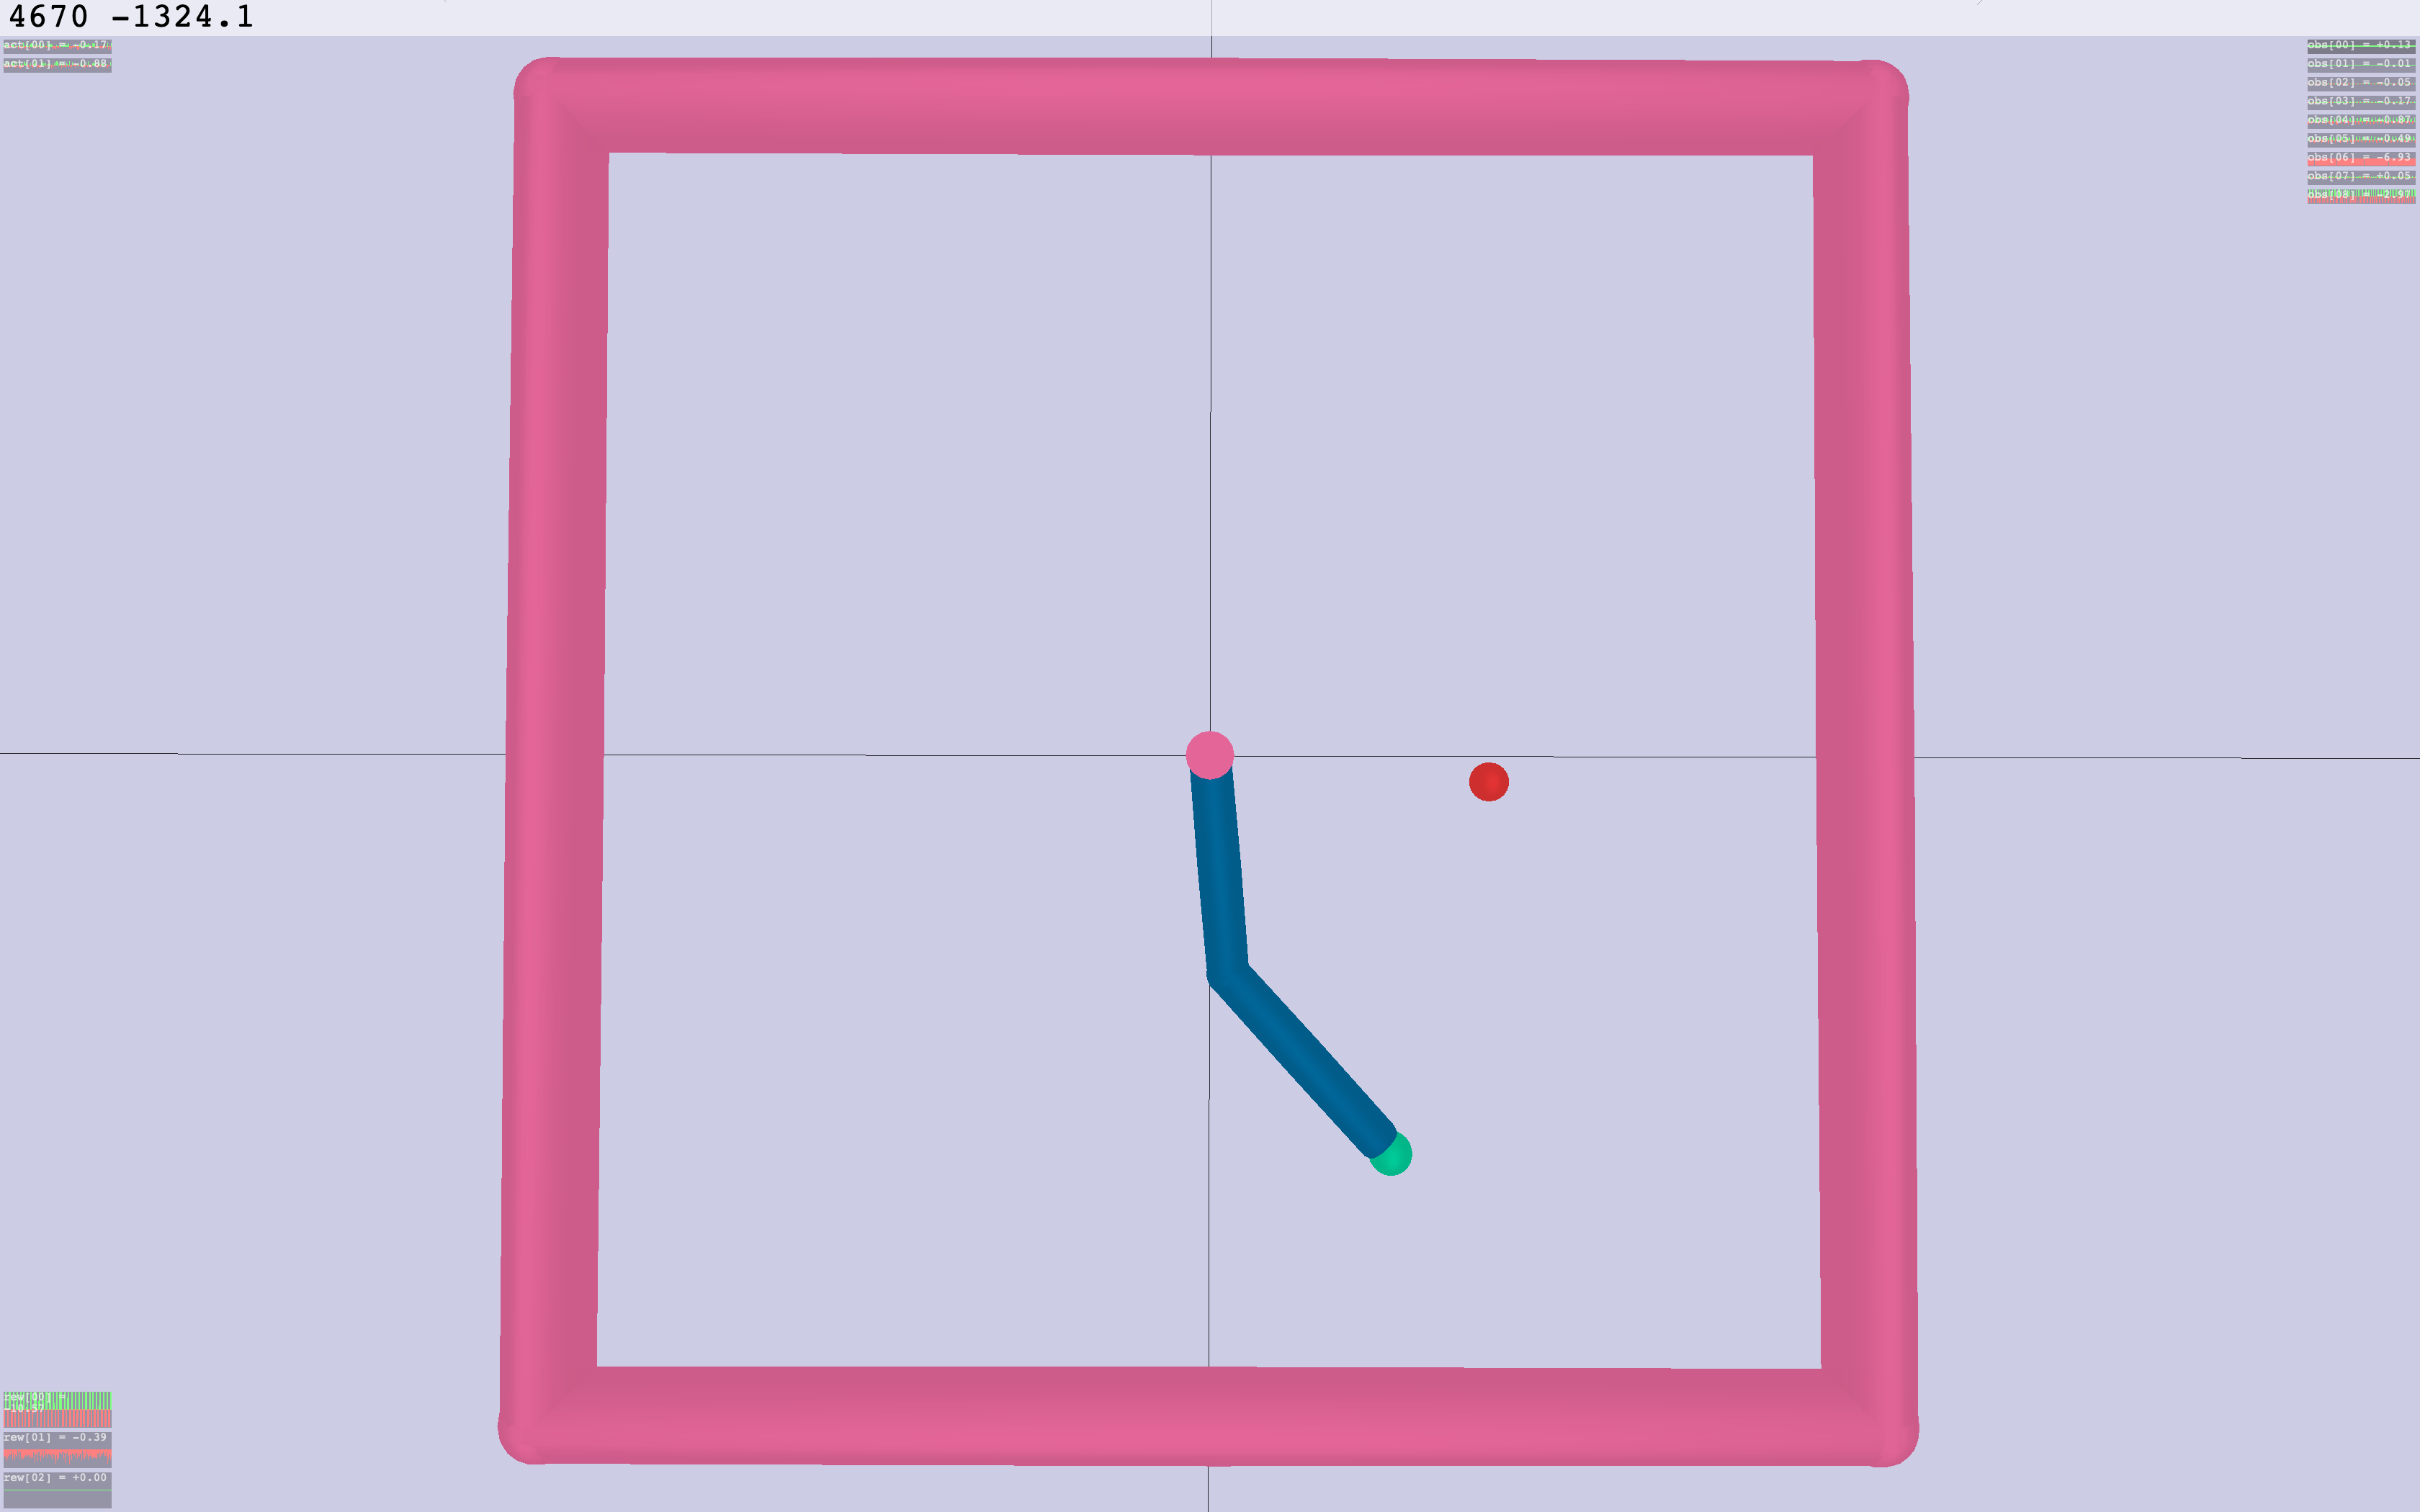
\includegraphics[width=0.7\linewidth]{figures/envs/openai_roboreacher.png}
            \caption{OpenAI Reacher Environment}
            \label{fig:openai_reacher}
    \end{center}
\end{figure}

\begin{table}[!htb]
    \centering
    \begin{subtable}{.4\linewidth}
        \centering
        \begin{tabular}{|c|c|}
        \hline
        \multicolumn{2}{|c|}{{\ul \textit{\textbf{Observation Space}}}}                                                                                   \\ \hline
        \multirow{2}{*}{\textbf{Target Position}}                                                                      & \textit{X Position}              \\ \cline{2-2} 
                                                                                                                    & \textit{Y Position}              \\ \hline
        \multirow{2}{*}{\textbf{Arm to Target Vector}}                                                                 & \textit{Position vector 0}       \\ \cline{2-2} 
                                                                                                                    & \textit{Position vector 1}       \\ \hline
        \multirow{2}{*}{\textbf{\begin{tabular}[c]{@{}c@{}}Current Relative Position\\ of Central Joint\end{tabular}}} & \textit{cosine of central joint} \\ \cline{2-2} 
                                                                                                                    & \textit{sine of central joint}   \\ \hline
        \multirow{2}{*}{\textbf{\begin{tabular}[c]{@{}c@{}}Current Relative Position\\ of Elbow Joint\end{tabular}}}   & \textit{cosine of elbow joint}   \\ \cline{2-2} 
                                                                                                                    & \textit{sine of elbow joint}     \\ \hline
        \end{tabular}
        \caption{Gym Reacher Observation Information}
        \label{tab:gym_reacher_obs}
    \end{subtable}%
    \hfill
    \begin{subtable}{.4\linewidth}
        \centering
        \begin{tabular}{|c|c|}
            \hline
            \multicolumn{2}{|c|}{{\ul \textit{\textbf{Action Space (Continuous)}}}}                             \\ \hline
            \multirow{2}{*}{\textbf{Center Joint Torque}} & \multirow{2}{*}{\textit{range(-1, 1)}} \\
                                                          &                                        \\ \hline
            \multirow{2}{*}{\textbf{Elbow Joint Torque}}  & \multirow{2}{*}{\textit{range(-1, 1)}} \\
                                                          &                                        \\ \hline
            \end{tabular}
            \caption{Gym Reacher Action Information}
            \label{tab:gym_reacher_actions}
    \end{subtable}%
    \caption{Gym Reacher Observation and Action Information}
\end{table}

the reward function is designed based on the distance between the arm and the target along with electricity cost of the torque and angular velocity of the arm with small epsilon amount in case of the joint is stuck. 

\clearpage

\textbf{Unity MLAgents: 2D and 3D Reacher Environment}

We have replicate the same openai gym reacher environment in unity to test the transferability between different physics engines, along with two 3d reacher environment (single and multi-agents) described below:

\textbf{Replicated Gym Env:}

\begin{figure}[H]
    \begin{center}
            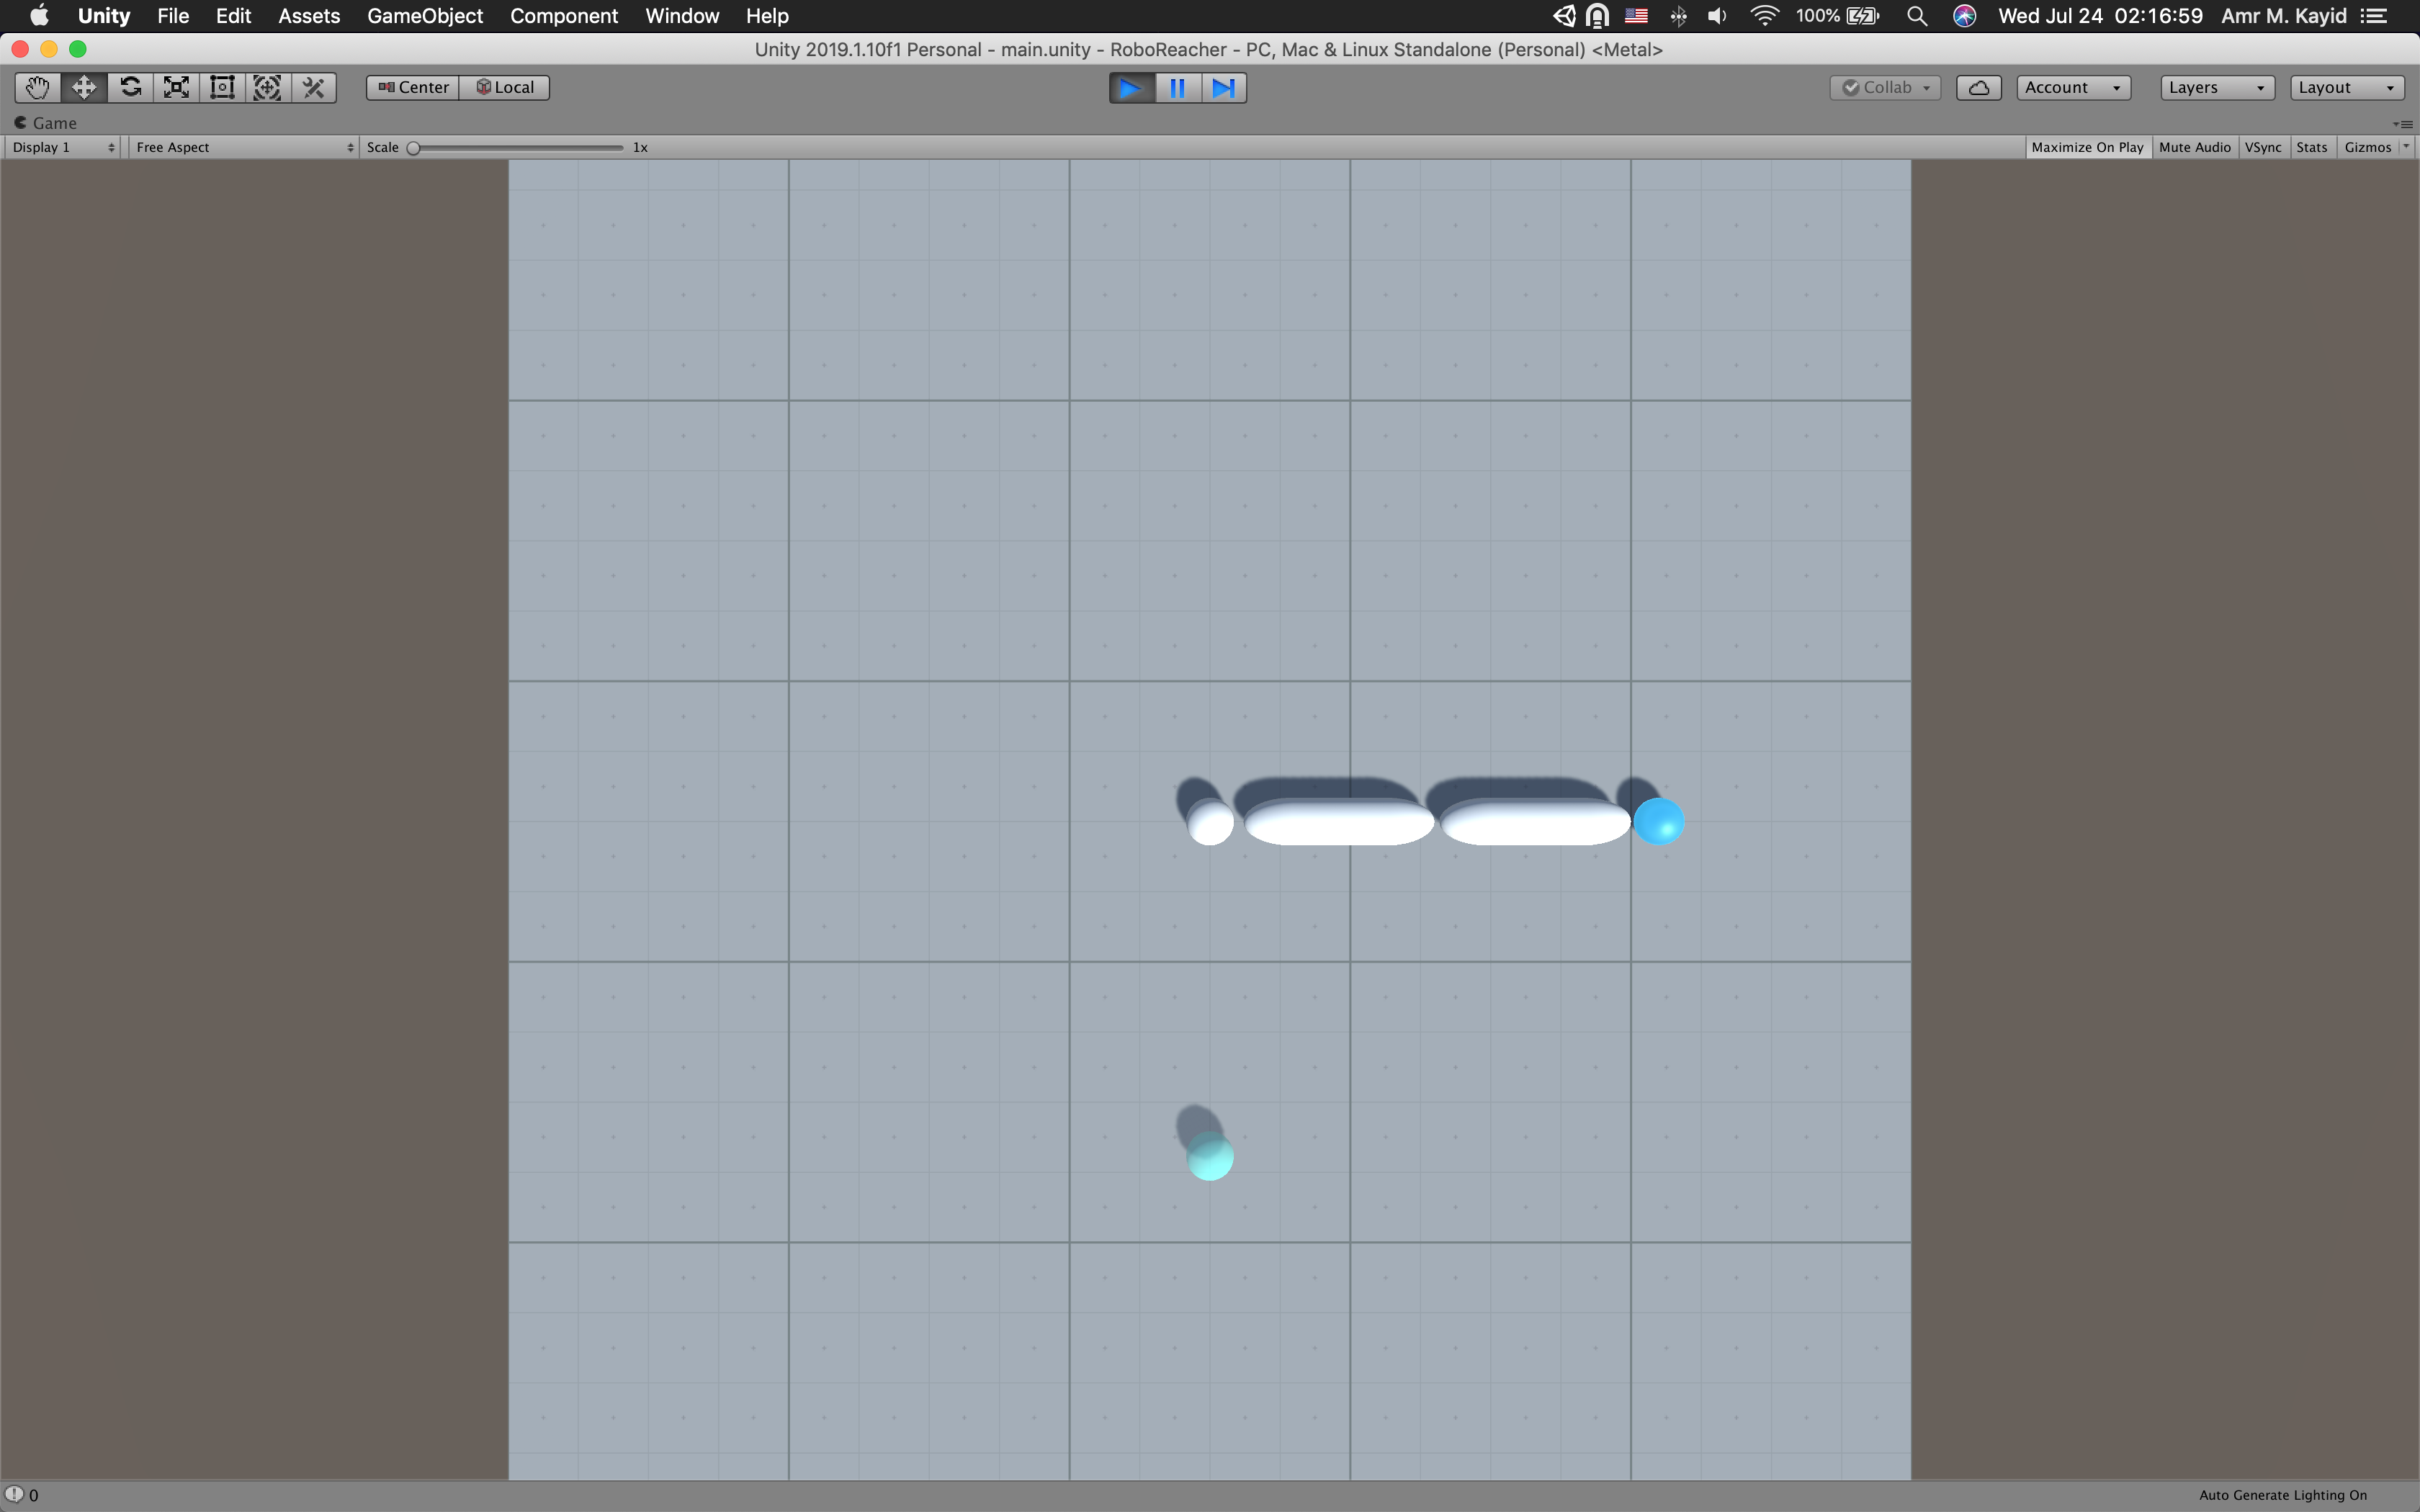
\includegraphics[width=0.7\linewidth]{figures/envs/unity_roboreacher.png}
            \caption{Replicated Gym Reacher Unity Environment}
            \label{fig:unity_reacher}
    \end{center}
\end{figure}


\textbf{Single Agent Reacher:} A robotic arm consist of two linked joints places in 3d plane surrounding it along with a moving sphere (target). The goal of the robotics arm it to reach target sphere and maintain following the point until the end of the episode. 

\begin{figure}[H]
    \begin{center}
            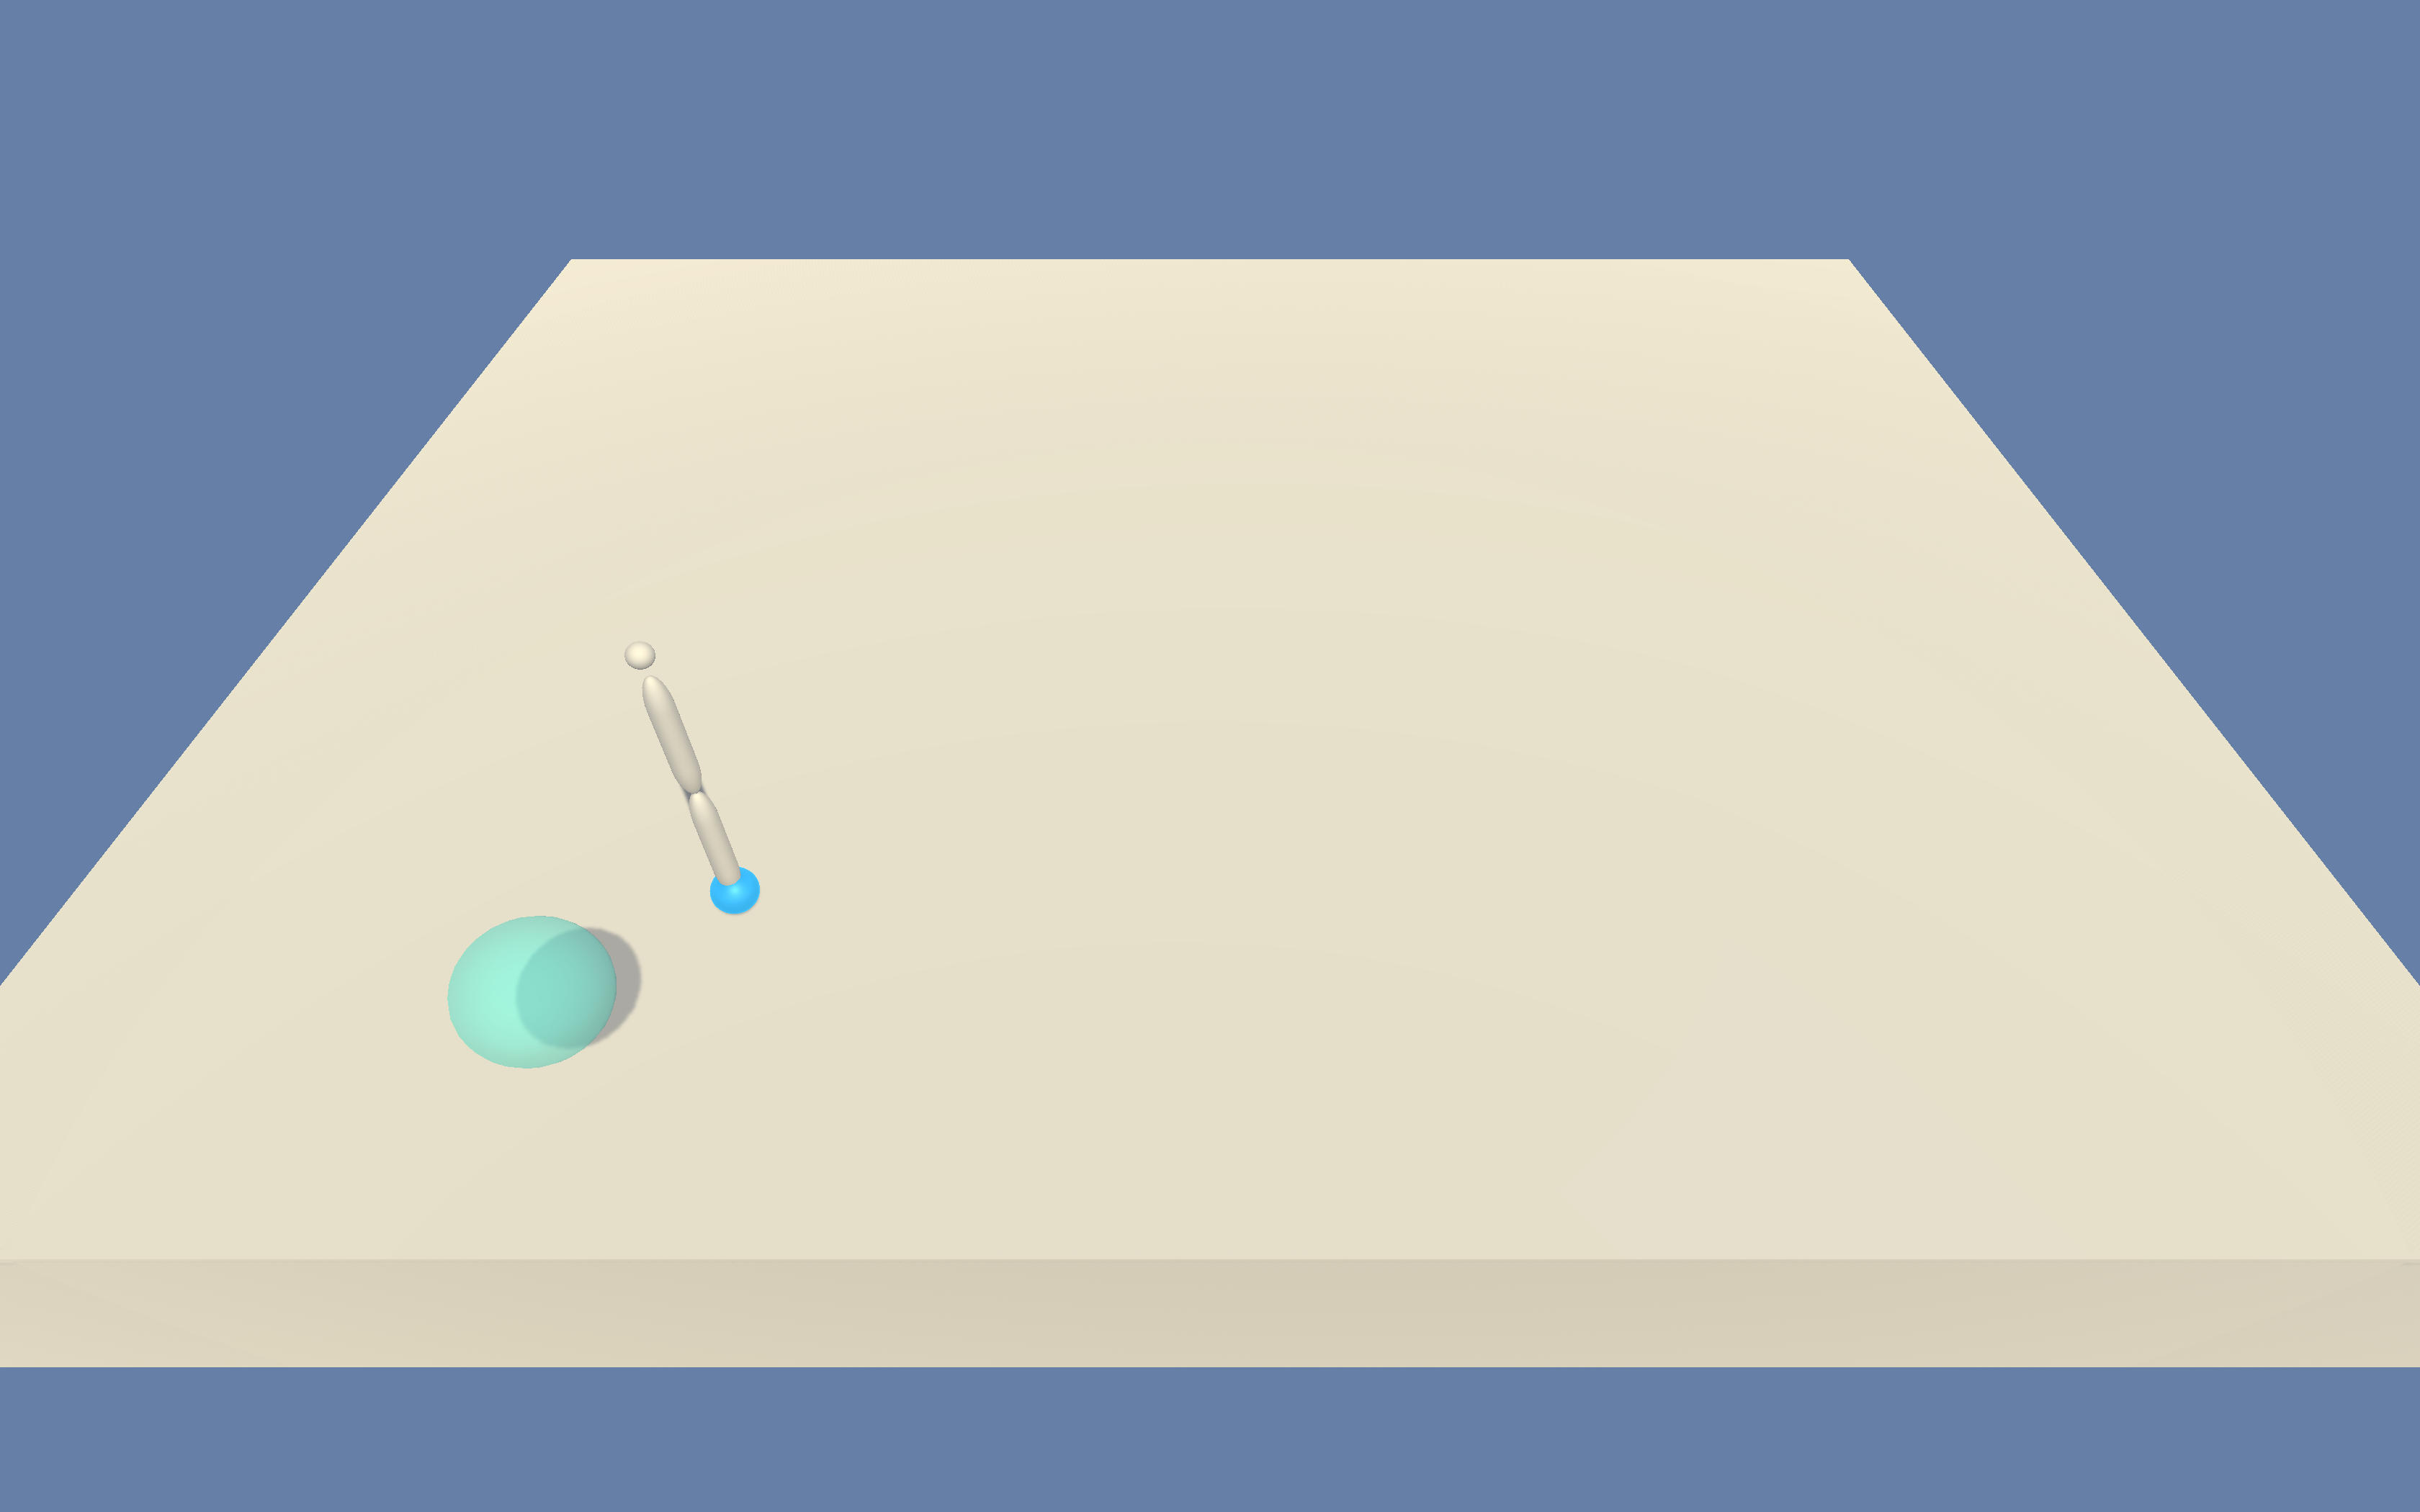
\includegraphics[width=0.7\linewidth]{figures/envs/unity_reacher_1.png}
            \caption{Unity Reacher Environment}
            \label{fig:unity_reacher_1}
    \end{center}
\end{figure}

\textbf{Multi-Agent Reacher:} in this environment, \textit{20 Agent} are used to parallelize the training process and collect more experiences and trajectories.

\begin{figure}[H]
    \begin{center}
            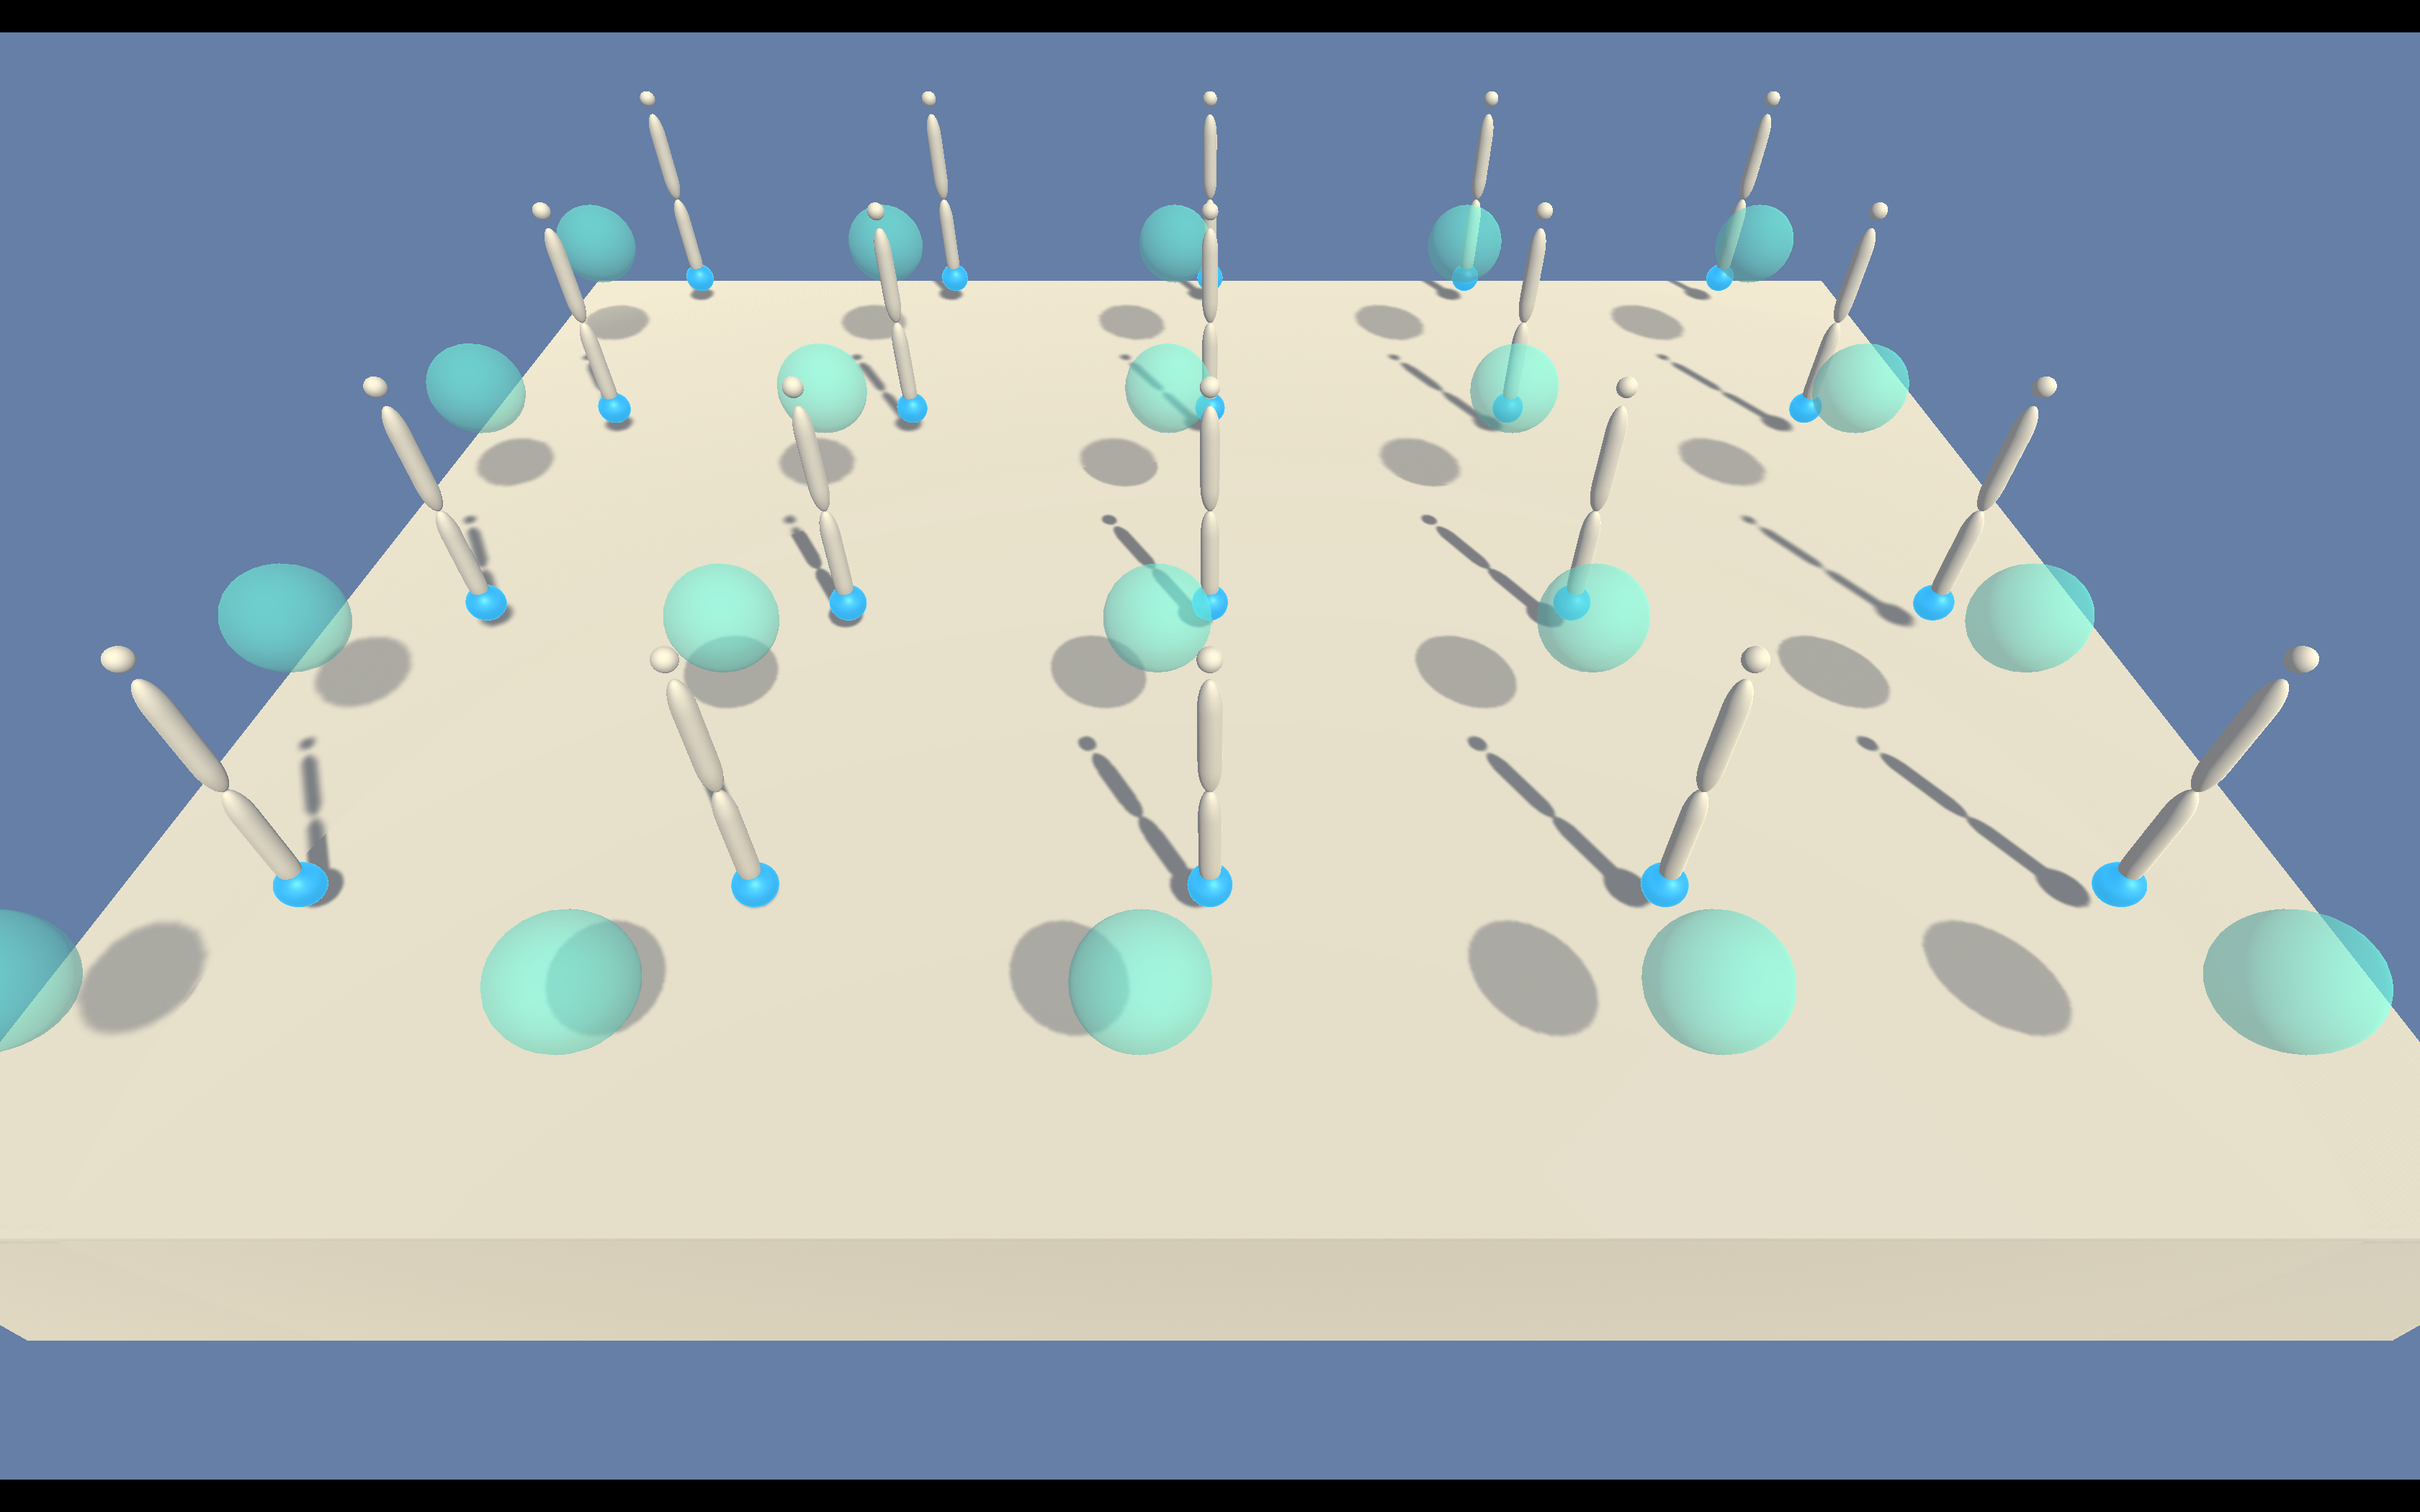
\includegraphics[width=0.7\linewidth]{figures/envs/unity_reacher_20.png}
            \caption{Unity Multi-Agent Reacher Environment}
            \label{fig:unity_reacher_20}
    \end{center}
\end{figure}

% !TeX root = ../../main.tex
% Add the above to each chapter to make compiling the PDF easier in some editors.

\chapter{Setup and Implementation}\label{chapter:setup_and_implementation}

In this chapter, the full details of the setups will be introduced. First, the used software framework will be presented. Then, our environments architecture and integration with the framework will be explained. Then, a brief description for the agents and algorithms will be shown. Lastly, description for all the used environments in our experiments will be provided.

\section{Overview}

Our approach is to setup a distributed learning architecture to run multiple experiments between selected environment and compare the results between training in normal non-distributed and distributed modes. We selected relatively close environment to robotics simulation with continuous observation and action spaces. A new abstract classes is introduced to run with the selected framework and unify the differences between different environments and physics simulators. A selection of the state of the art algorithms is used to train our reinforcement learning agents and compare between the algorithm and the modes for each algorithm.

\section{Software}
\textbf{Ray Framework~\parencite{moritz2018ray}: } Ray is a fast and simple framework for building and running distributed applications. The same code can be run on a single machine to achieve efficient multiprocessing, and it can be used on a cluster for large computations. Ray provide high scalability and a unified API for a variety of applications which is very useful for our experiments. Ray executes tasks asynchronously to achieve parallelism enabling us to run multiple environments in the same experiment to benefit from collection more experiences and trajectories for the agent.

\textbf{OpenAI Gym~\parencite{brockman2016openai}: } openai gym is a toolkit for developing and comparing reinforcement learning algorithms. It supports teaching agents everything from walking to playing games like Pong or Pinball. It has an open source interface to reinforcement learning tasks which provides an easy-to-use suite of reinforcement learning tasks. 

The core gym interface is \textbf{Env}, which is the unified environment interface. 
The following are the methods for the abstracted gym Env:

\begin{itemize}
    \item \textit{\textbf{\colorbox{gray!20}{reset(self)}}}: Reset the environment's state. Returns observation.
    \item \textit{\textbf{\colorbox{gray!20}{step(self, action)}}}: Step the environment by one time-step. Returns observation, reward, done, info.
    \item \textit{\textbf{\colorbox{gray!20}{render(self, mode='human')}}}: Render one frame of the environment. The default mode will do something human friendly, such as pop up a window.
\end{itemize}

\textbf{Unity MLAgents~\parencite{juliani2018unity}: } unity mlagents toolkit is an open-source Unity plugin that enables games and simulations to serve as environments for training intelligent agents. It has more realistic and complex simulation environments. It provides the ability to flexibly configure
the simulation. By taking advantage of Unity as a simulation platform, the toolkit enables the development of learning environments which are rich in sensory and physical complexity, provide compelling cognitive challenges, and support dynamic multi-agent interaction. Agents can be trained using reinforcement learning, imitation learning, neuroevolution, or other machine learning methods through a simple-to-use Python API. They provide implementations of state-of-the-art algorithms to enable game developers and hobbyists to easily train intelligent agents for 2D, 3D and VR/AR games. We are using this to test running multiple agents in the same environment and compare the effect with one agent only. Also, to experiment the transferability between different physics simulators.

\section{Architecture}

At a high level, ray provides an \textbf{\colorbox{gray!20}{Trainer}} class which holds a policy for environment interaction. Through the trainer interface~\ref{fig:ray_trainer}, the policy can be trained, check-pointed, or an action computed. In multi-agent training, the trainer manages the querying and optimization of multiple policies at once. It provides custom resources configurations~\ref{fig:ray_config}, which can control the degree of parallelism used by setting the \colorbox{gray!20}{\texttt{num\_workers}} hyper-parameter for most algorithms. The number of GPUs the driver should use can be set via the \colorbox{gray!20}{\texttt{num\_gpus}} option. Similarly, the resource allocation to workers can be controlled via \colorbox{gray!20}{\texttt{num\_cpus\_per\_worker}}, \colorbox{gray!20}{\texttt{num\_gpus\_per\_worker}}, and \colorbox{gray!20}{\texttt{custom\_resources\_per\_worker}}. The number of GPUs can be a fractional quantity to allocate only a fraction of a GPU. For example, with DQN you can pack five trainers onto one GPU by setting \colorbox{gray!20}{\texttt{num\_gpus}: 0.2}.

\begin{figure}[H]
	\centering
	\begin{subfigure}[b]{0.4\textwidth}
		\centering
		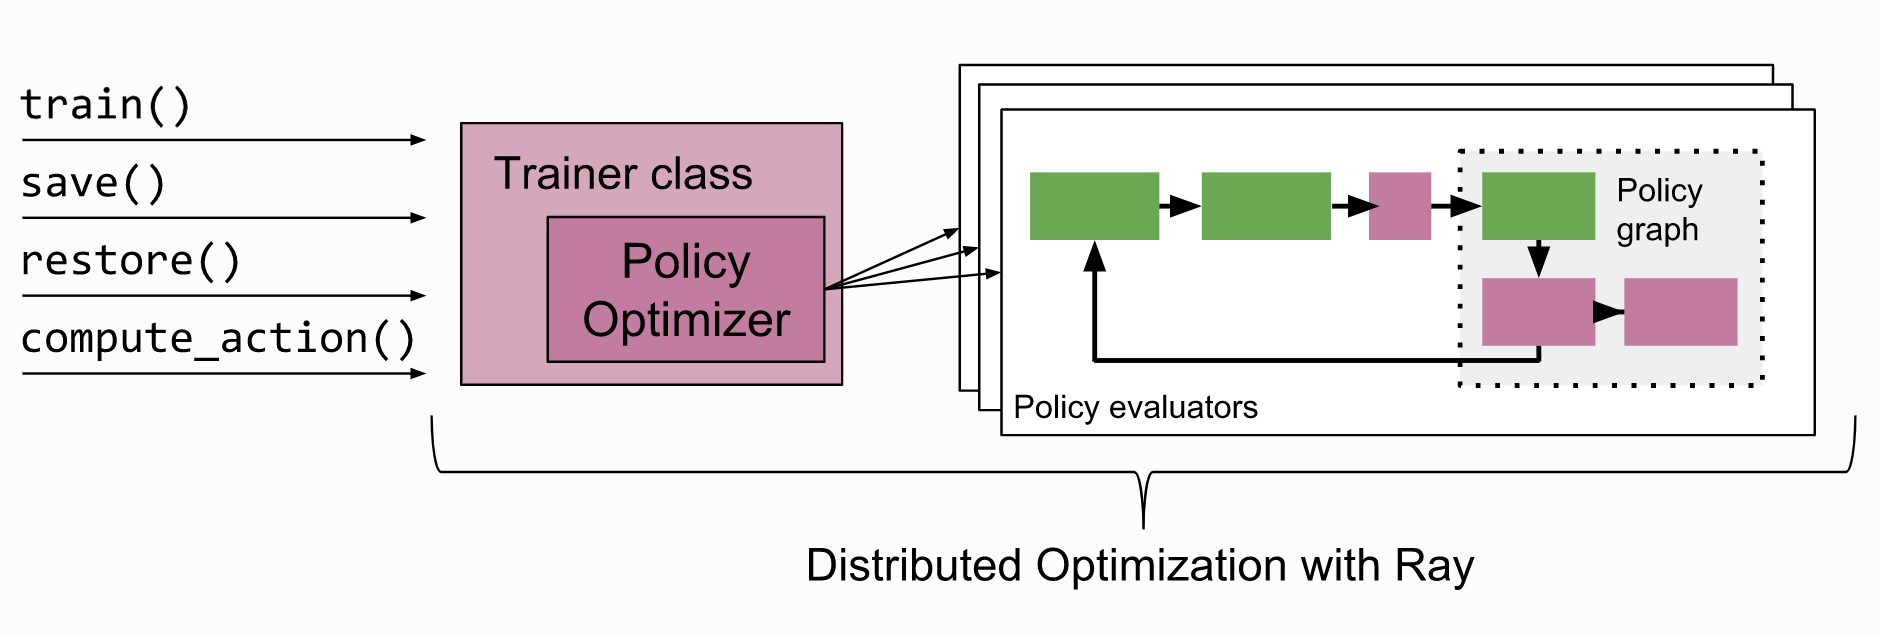
\includegraphics[width=\textwidth]{figures/architecture/ray_trainer.png}
		\caption{Ray Training Process}
		\label{fig:ray_trainer}
    \end{subfigure}
    \hfill
	\begin{subfigure}[b]{0.4\textwidth}
		\centering
		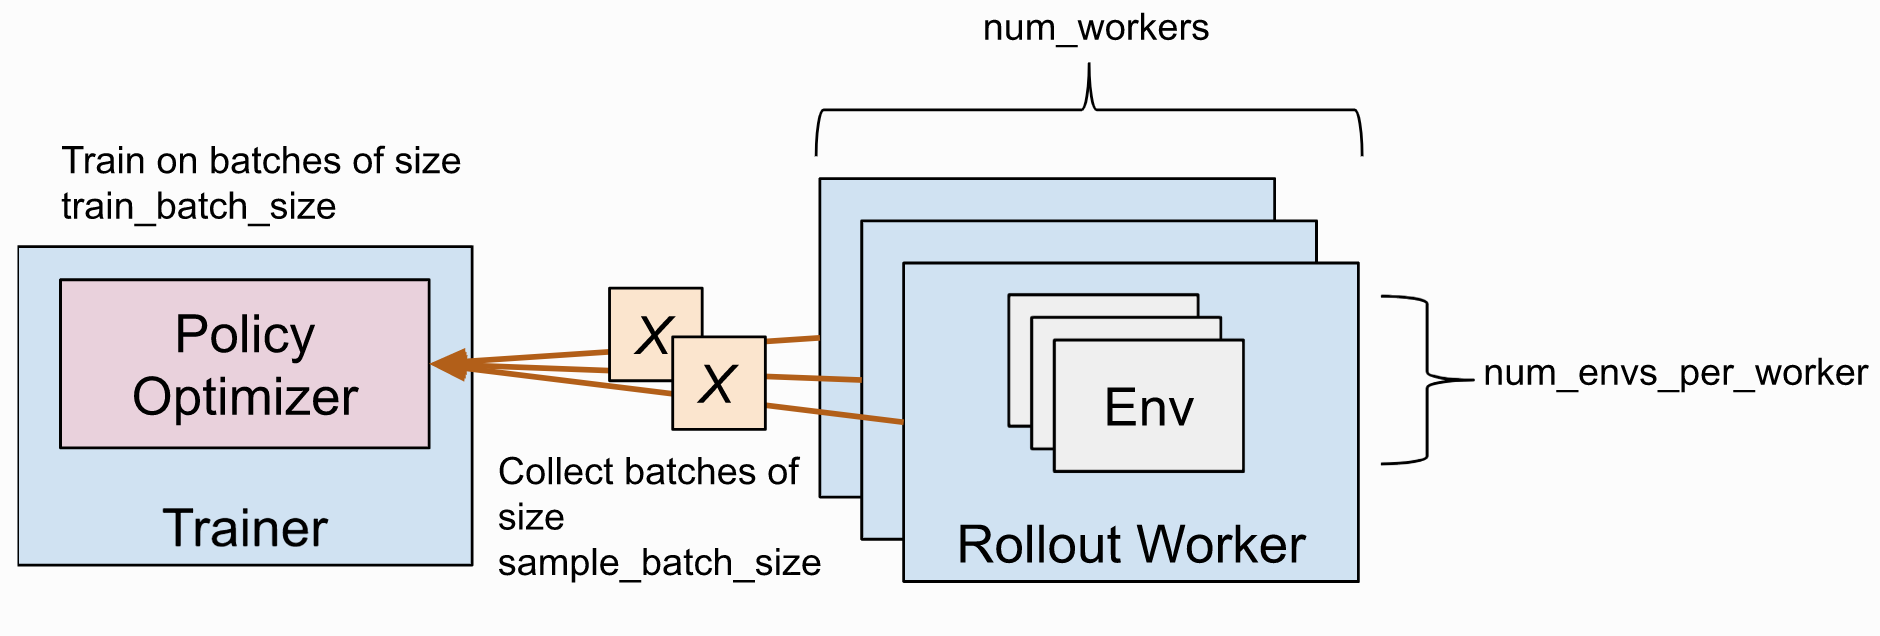
\includegraphics[width=\textwidth]{figures/architecture/ray_config.png}
        \caption{Ray Configurable resources}
		\label{fig:ray_config}
	\end{subfigure}
	\hfill
	   \caption{General Overview of Ray framework~\parencite{moritz2018ray}}
	   \label{fig:ray}
\end{figure}

Since ray support only OpenAI Gym environments along with their provided multi-agent and also batched environments, we had to implement our custom environment to unify between unity mlagents and openai gym environments. Also, we implemented our custom Multi-Agent environments for both used environments as shown in the following figure~\ref{fig:ray_envs}.

\begin{figure}[H]
	\centering
		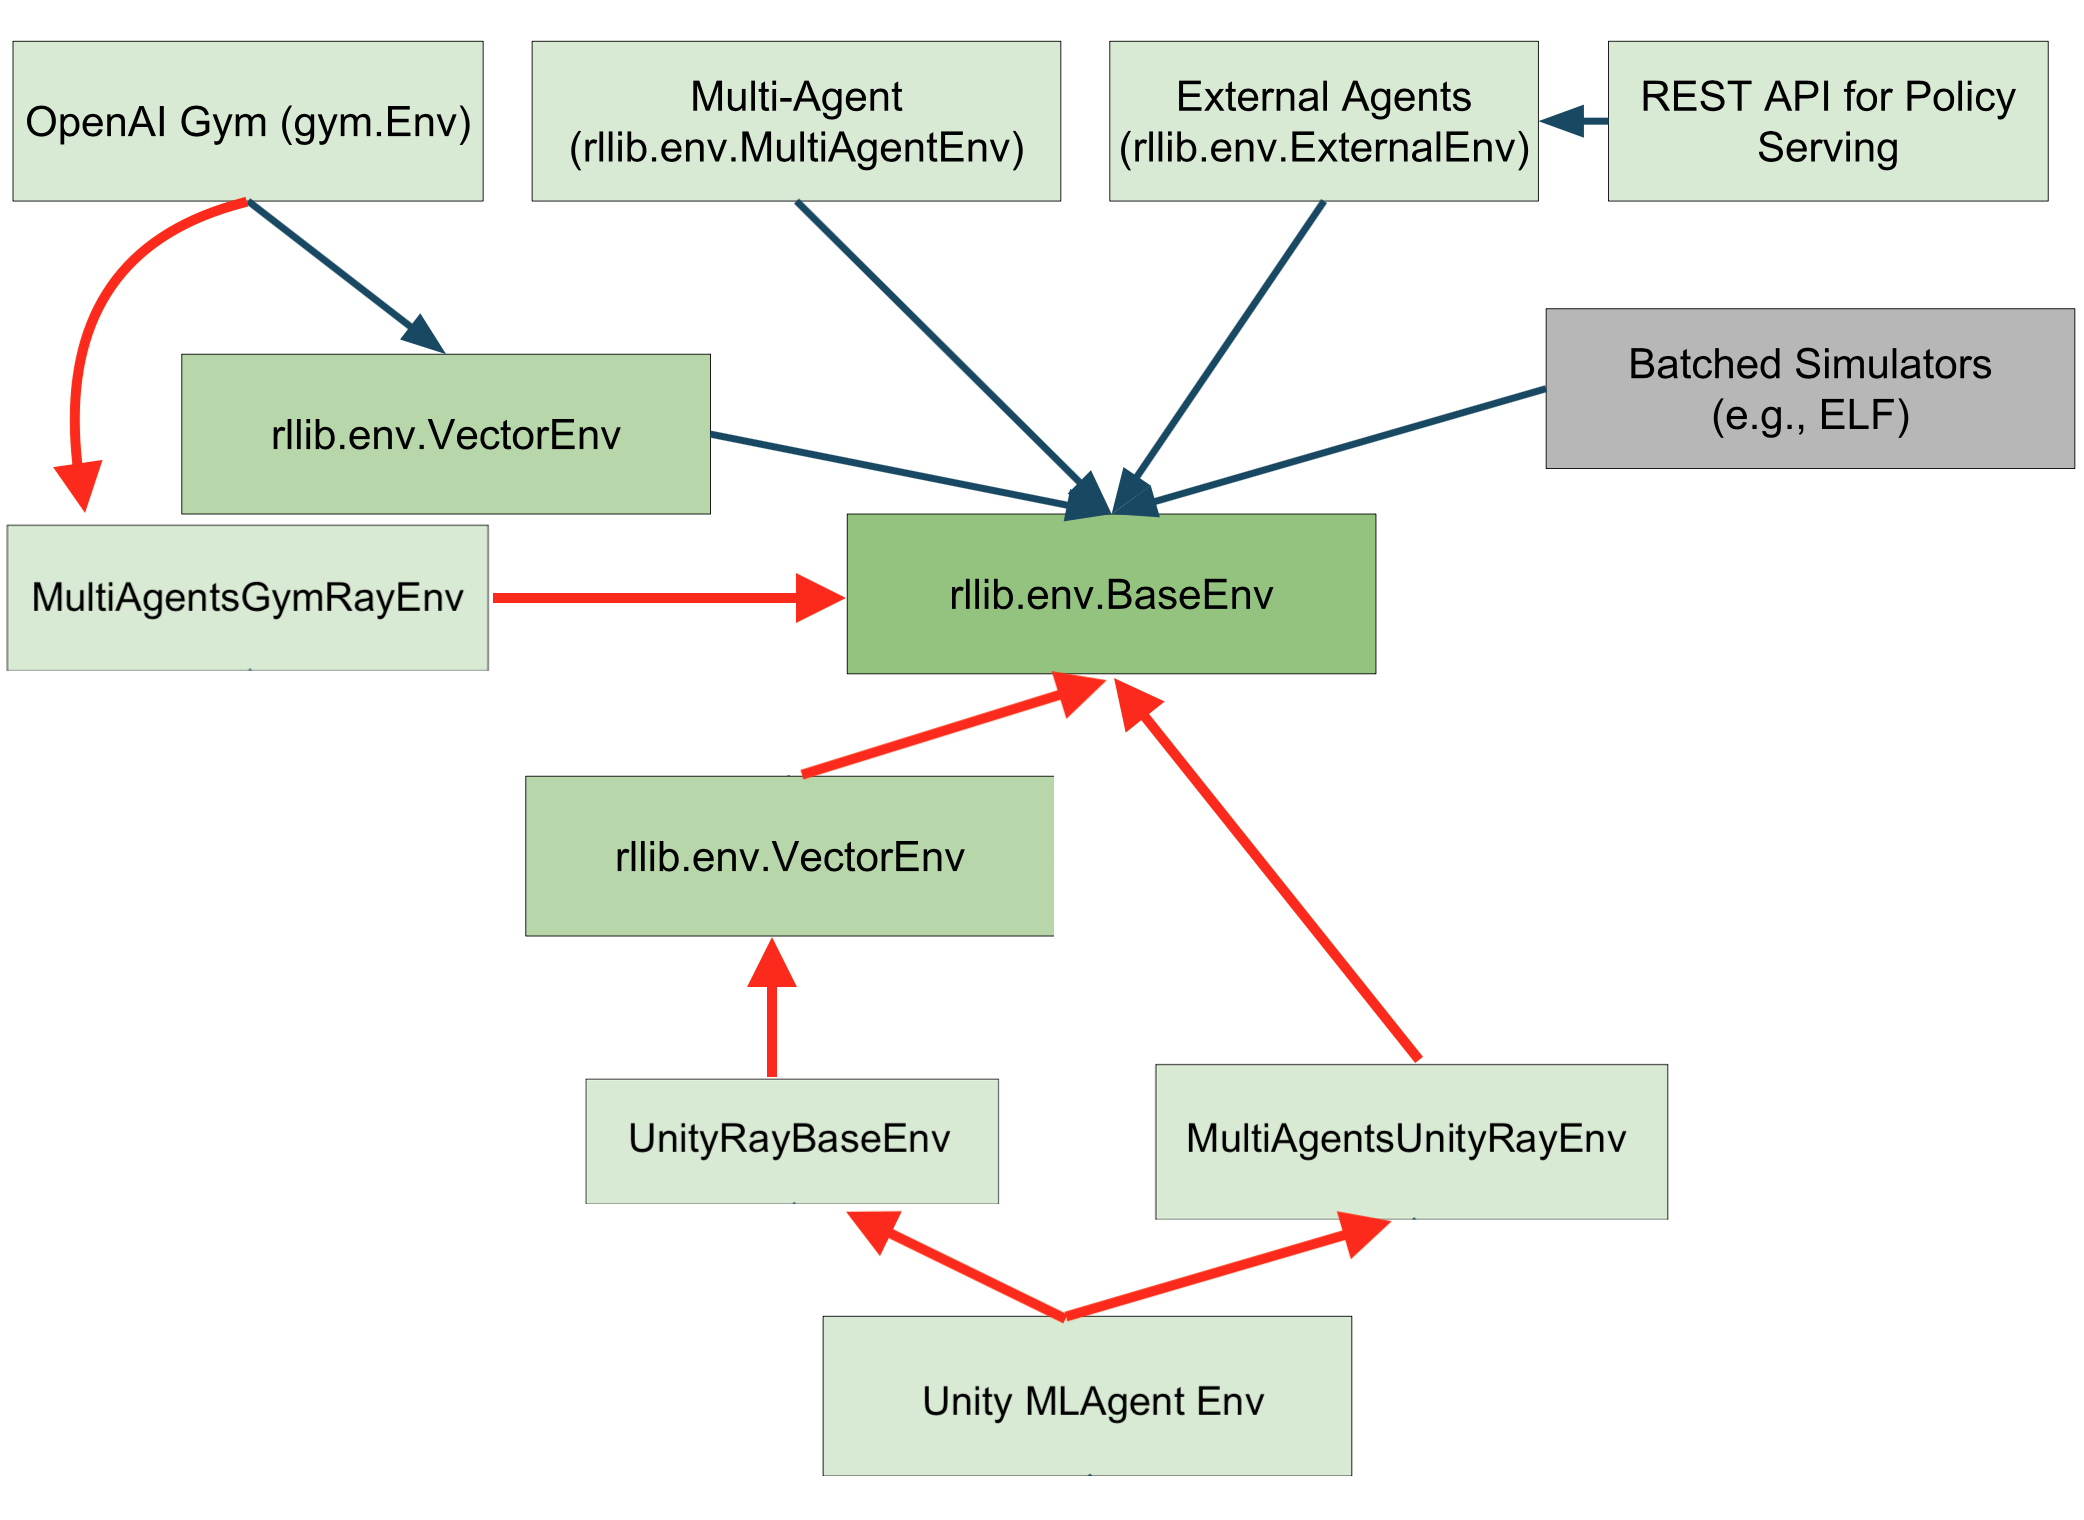
\includegraphics[width=\linewidth]{figures/architecture/ray_envs.png}
		\caption{Our Custom Environments}
		\label{fig:ray_envs}
\end{figure}

\clearpage

Custom environments implementations and methods are described below:

\textbf{UnityRayEnv}:\\
our base unity environment maps the observations and actions from unity mlagents toolkit to be compatible with Ray BaseEnv. Since unity mlagents deals with brains that control the agents and the environments we had to convert it to the required \colorbox{gray!20}{\texttt{observation\_space}} and \colorbox{gray!20}{\texttt{action\_space}} for ray env with the following methods:
\begin{itemize}
    \item \textit{\textbf{\colorbox{gray!20}{\texttt{\_\_init\_\_(self)}}}}: Create the unity environment from the unity build env, convert the observation and action spaces to be ray-compatible.
    \item \textit{\textbf{\colorbox{gray!20}{reset(self)}}}: Reset the environment's state. Returns observation.
    \item \textit{\textbf{\colorbox{gray!20}{step(self, action)}}}: Step the environment by one time-step. Returns observation, reward, done, info.
\end{itemize}

\textbf{MultiAgentsUnityRayEnv}:\\
this class inherit from both \colorbox{gray!20}{\textbf{UnityRayEnv}} and \colorbox{gray!20}{\textbf{MultiAgentEnv}}~\ref{fig:ray_multiagentenv}. The difference from the base environment is in both methods \textit{\textbf{\colorbox{gray!20}{reset(self)}}} and \textit{\textbf{\colorbox{gray!20}{step(self, \texttt{actions\_dict})}}}, where the reset function reset all the observations for each agent that exist in the environment and step function take a dictionary of actions corresponding for each action of a single agent. The same applies to \textbf{MultiAgentsGymRayEnv}.

\begin{figure}[H]
	\centering
		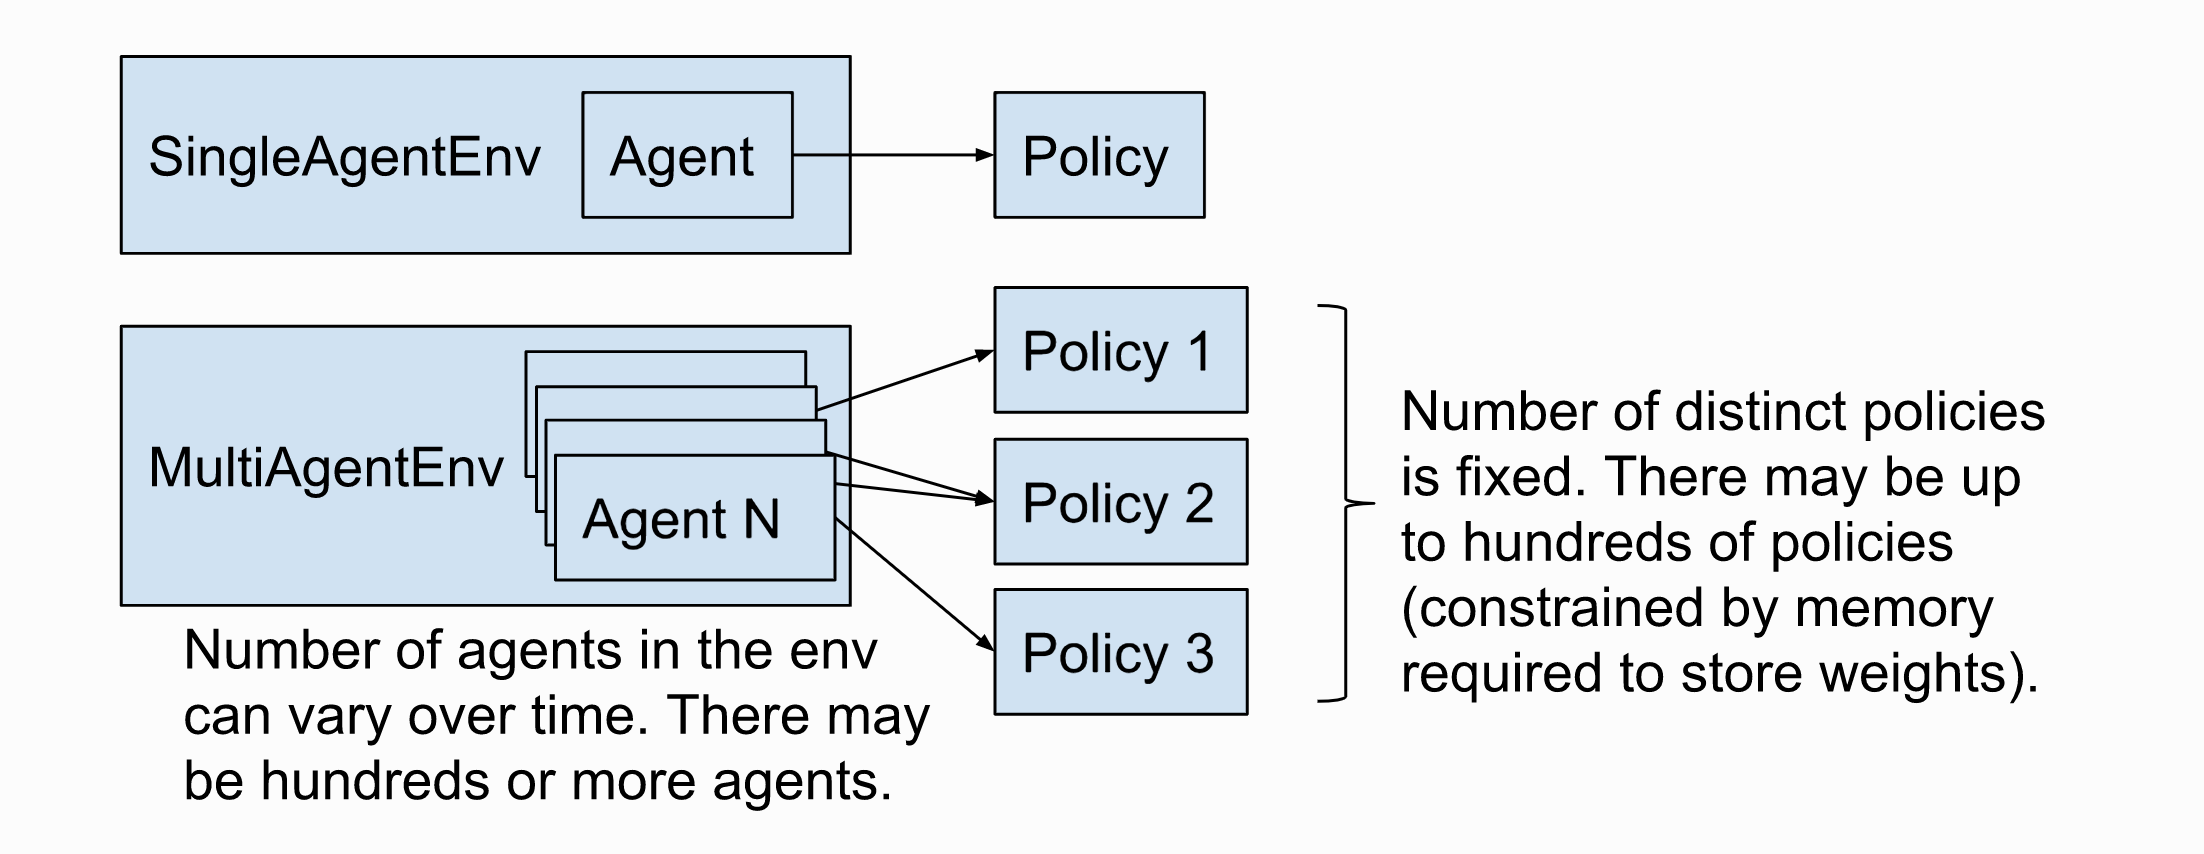
\includegraphics[width=\linewidth]{figures/architecture/ray_multiagentenv.png}
		\caption{Ray MultiAgentEnv}
		\label{fig:ray_multiagentenv}
\end{figure}

\section{Agents and Algorithms}

\begin{itemize}
    \item \textbf{Proximal Policy Optimization (PPO)}: PPO’s clipped objective supports multiple SGD passes over the same batch of experiences. RLlib’s multi-GPU optimizer pins that data in GPU memory to avoid unnecessary transfers from host memory, substantially improving performance over a naive implementation. RLlib’s PPO scales out using multiple workers for experience collection, and also with multiple GPUs for SGD.

    \item \textbf{Distributed Prioritized Experience Replay (Ape-X)}: Ape-X variations of DQN, DDPG, use a single GPU learner and many CPU workers for experience collection. Experience collection can scale to hundreds of CPU workers due to the distributed prioritization of experience prior to storage in replay buffers.

    \item \textbf{Importance Weighted Actor-Learner Architecture (IMPALA)}: In IMPALA, a central learner runs SGD in a tight loop while asynchronously pulling sample batches from many actor processes. RLlib’s IMPALA implementation uses DeepMind’s reference V-trace code. Note that we do not provide a deep residual network out of the box, but one can be plugged in as a custom model. Multiple learner GPUs and experience replay are also supported.
\end{itemize}

\section{Environments and Tasks Description}
Our task is robotic related task, where we have a robotic arm consist of two linked joints \textit{(agent)} and moving sphere \textit{(target)}. The robotic arm and the goal differ according to the environment used. We have a one experiment where is the agent movement is in 2D and the goal of the agent it to reach the target as fast as possible to maximize the given cumulative reward. In the second experiment, the agent can move in 3D and the goal is to keep track of the moving target and move with it along the 3D space.

Following is detailed description for all the environment used in our experiments.

\textbf{OpenAI: Reacher Environment}

Our first and baseline environment is \textit{Reacher Environment}~\ref{fig:openai_reacher}: A robotic arm consist of two linked joints places in a squared arena surrounding it along with a moving sphere (target). The goal of the robotics arm it to reach target sphere and maintain following the point until the end of the episode. 

\begin{figure}[H]
    \begin{center}
            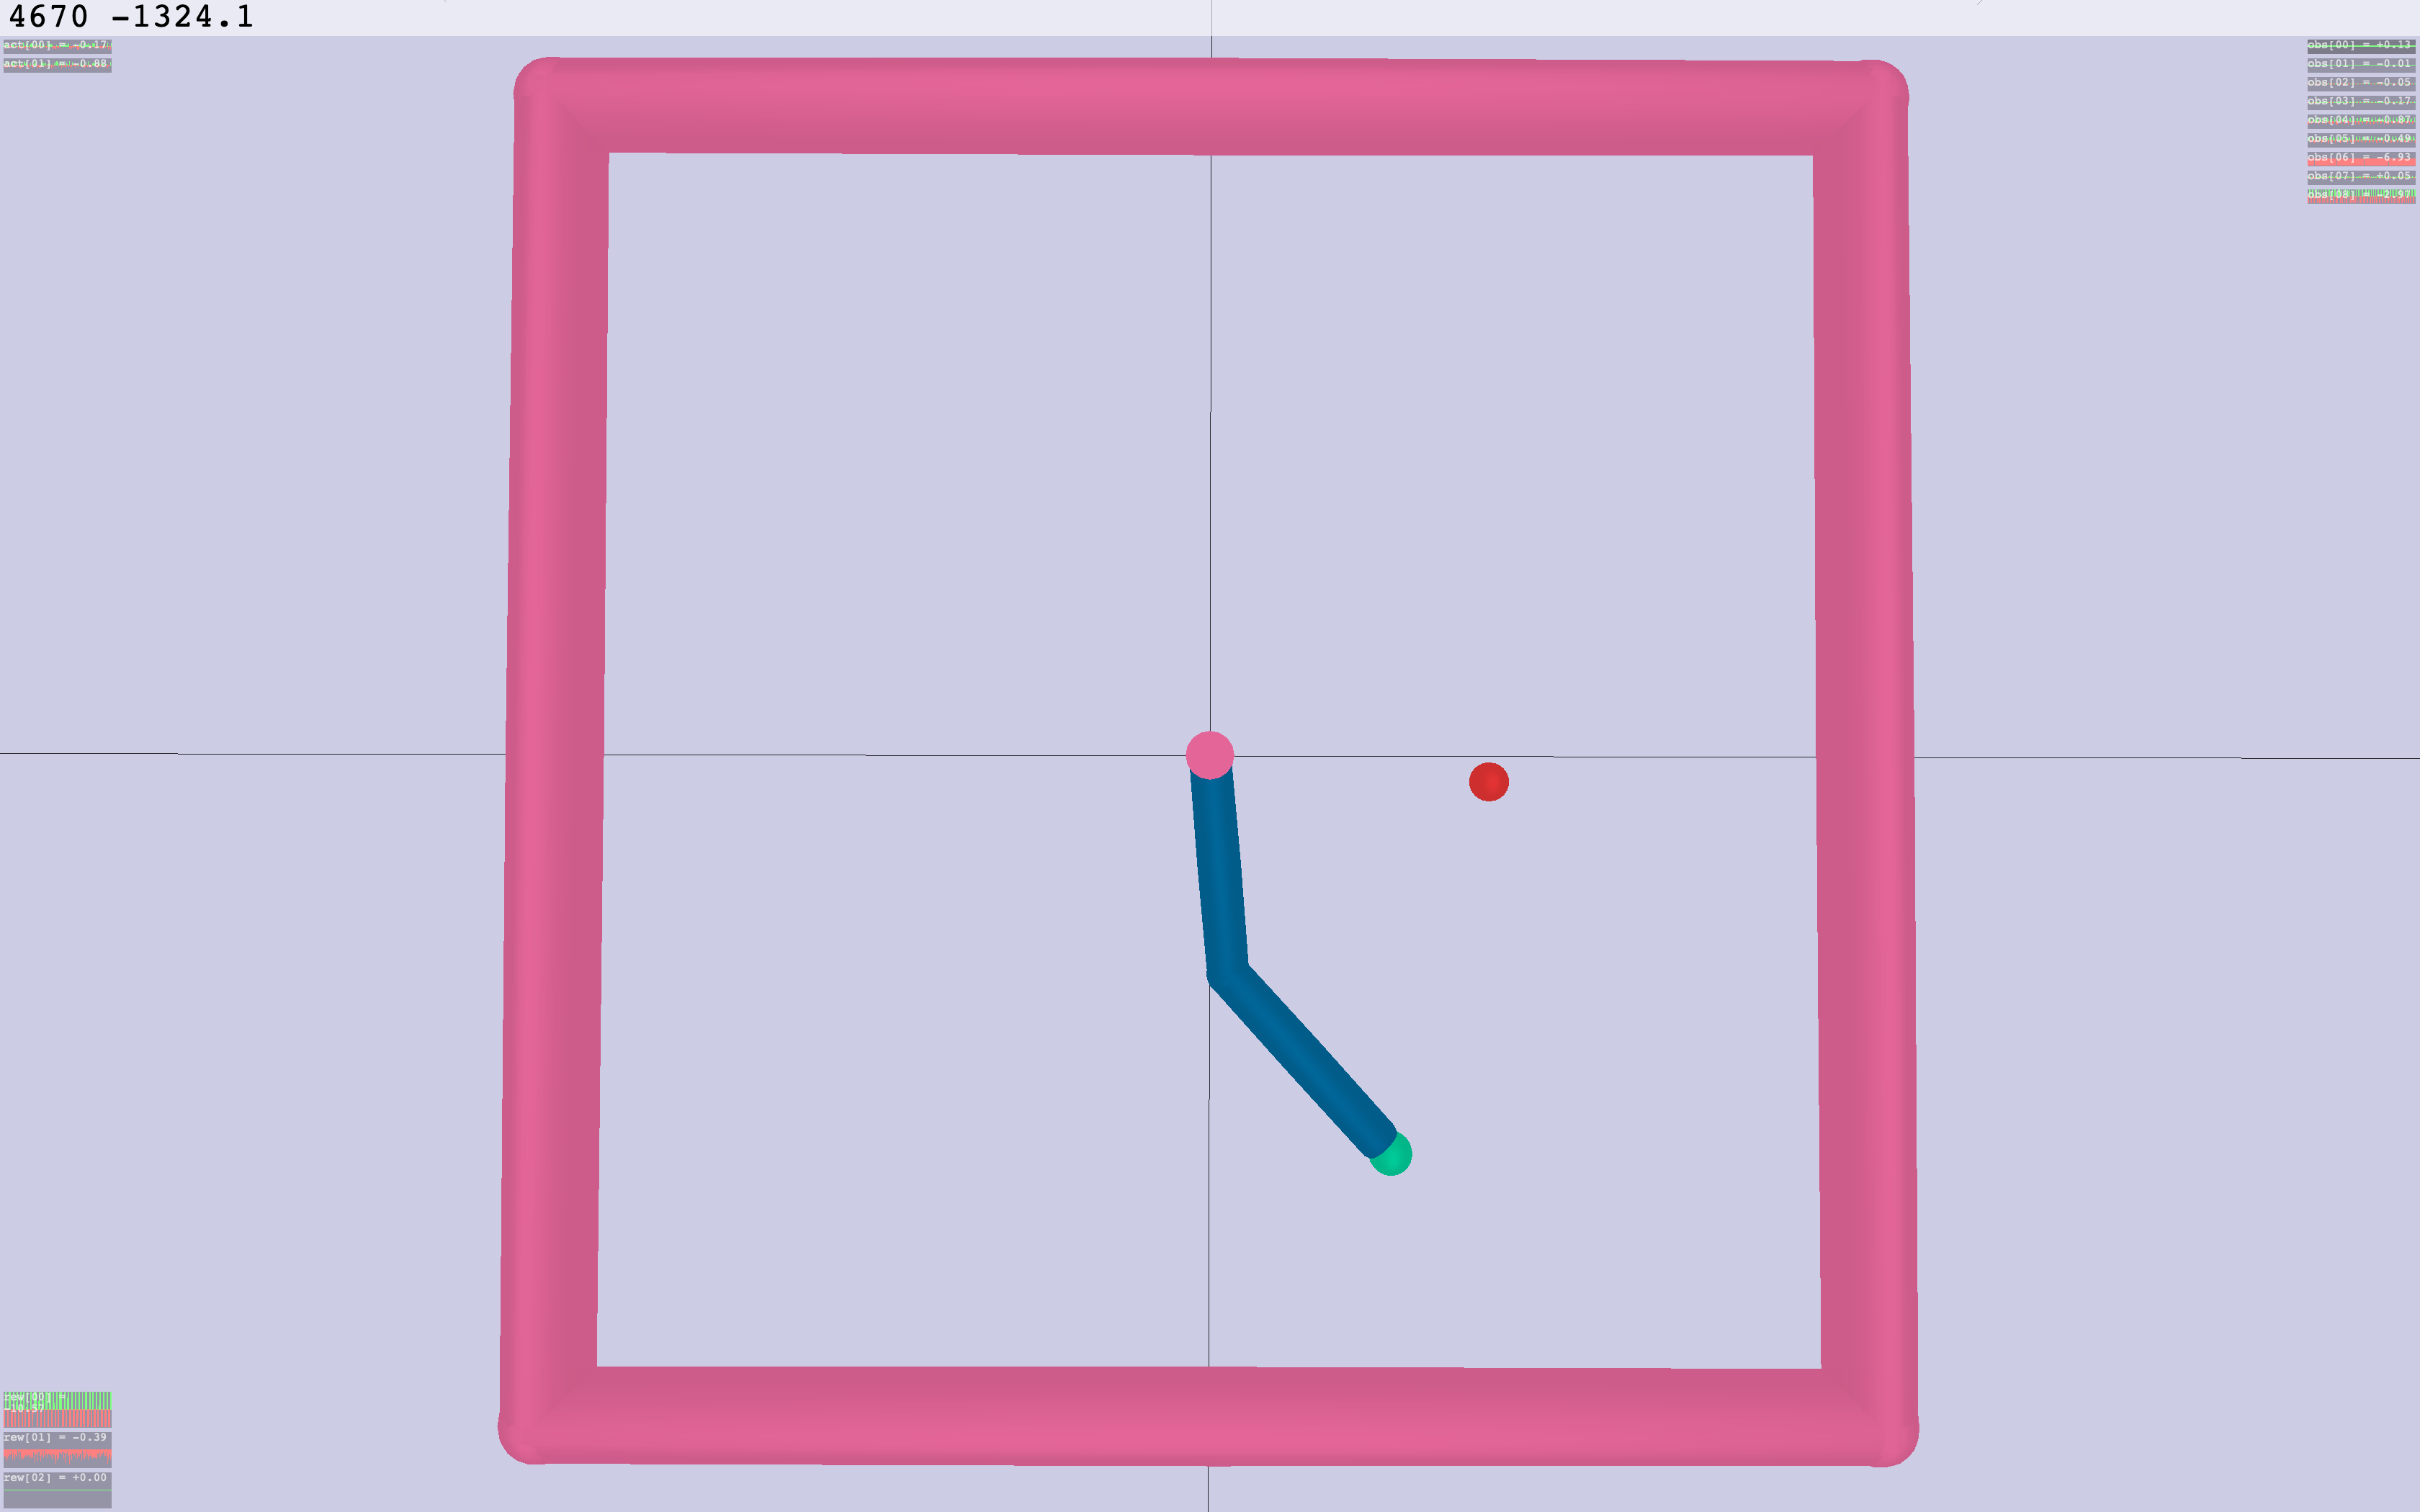
\includegraphics[width=0.7\linewidth]{figures/envs/openai_roboreacher.png}
            \caption{OpenAI Reacher Environment}
            \label{fig:openai_reacher}
    \end{center}
\end{figure}

\begin{table}[!htb]
    \centering
    \begin{subtable}{.4\linewidth}
        \centering
        \begin{tabular}{|c|c|}
        \hline
        \multicolumn{2}{|c|}{{\ul \textit{\textbf{Observation Space}}}}                                                                                   \\ \hline
        \multirow{2}{*}{\textbf{Target Position}}                                                                      & \textit{X Position}              \\ \cline{2-2} 
                                                                                                                    & \textit{Y Position}              \\ \hline
        \multirow{2}{*}{\textbf{Arm to Target Vector}}                                                                 & \textit{Position vector 0}       \\ \cline{2-2} 
                                                                                                                    & \textit{Position vector 1}       \\ \hline
        \multirow{2}{*}{\textbf{\begin{tabular}[c]{@{}c@{}}Current Relative Position\\ of Central Joint\end{tabular}}} & \textit{cosine of central joint} \\ \cline{2-2} 
                                                                                                                    & \textit{sine of central joint}   \\ \hline
        \multirow{2}{*}{\textbf{\begin{tabular}[c]{@{}c@{}}Current Relative Position\\ of Elbow Joint\end{tabular}}}   & \textit{cosine of elbow joint}   \\ \cline{2-2} 
                                                                                                                    & \textit{sine of elbow joint}     \\ \hline
        \end{tabular}
        \caption{Gym Reacher Observation Information}
        \label{tab:gym_reacher_obs}
    \end{subtable}%
    \hfill
    \begin{subtable}{.4\linewidth}
        \centering
        \begin{tabular}{|c|c|}
            \hline
            \multicolumn{2}{|c|}{{\ul \textit{\textbf{Action Space (Continuous)}}}}                             \\ \hline
            \multirow{2}{*}{\textbf{Center Joint Torque}} & \multirow{2}{*}{\textit{range(-1, 1)}} \\
                                                          &                                        \\ \hline
            \multirow{2}{*}{\textbf{Elbow Joint Torque}}  & \multirow{2}{*}{\textit{range(-1, 1)}} \\
                                                          &                                        \\ \hline
            \end{tabular}
            \caption{Gym Reacher Action Information}
            \label{tab:gym_reacher_actions}
    \end{subtable}%
    \caption{Gym Reacher Observation and Action Information}
\end{table}

the reward function is designed based on the distance between the arm and the target along with electricity cost of the torque and angular velocity of the arm with small epsilon amount in case of the joint is stuck. 

\clearpage

\textbf{Unity MLAgents: 2D and 3D Reacher Environment}

We have replicate the same openai gym reacher environment in unity to test the transferability between different physics engines, along with two 3d reacher environment (single and multi-agents) described below:

\textbf{Replicated Gym Env:}

\begin{figure}[H]
    \begin{center}
            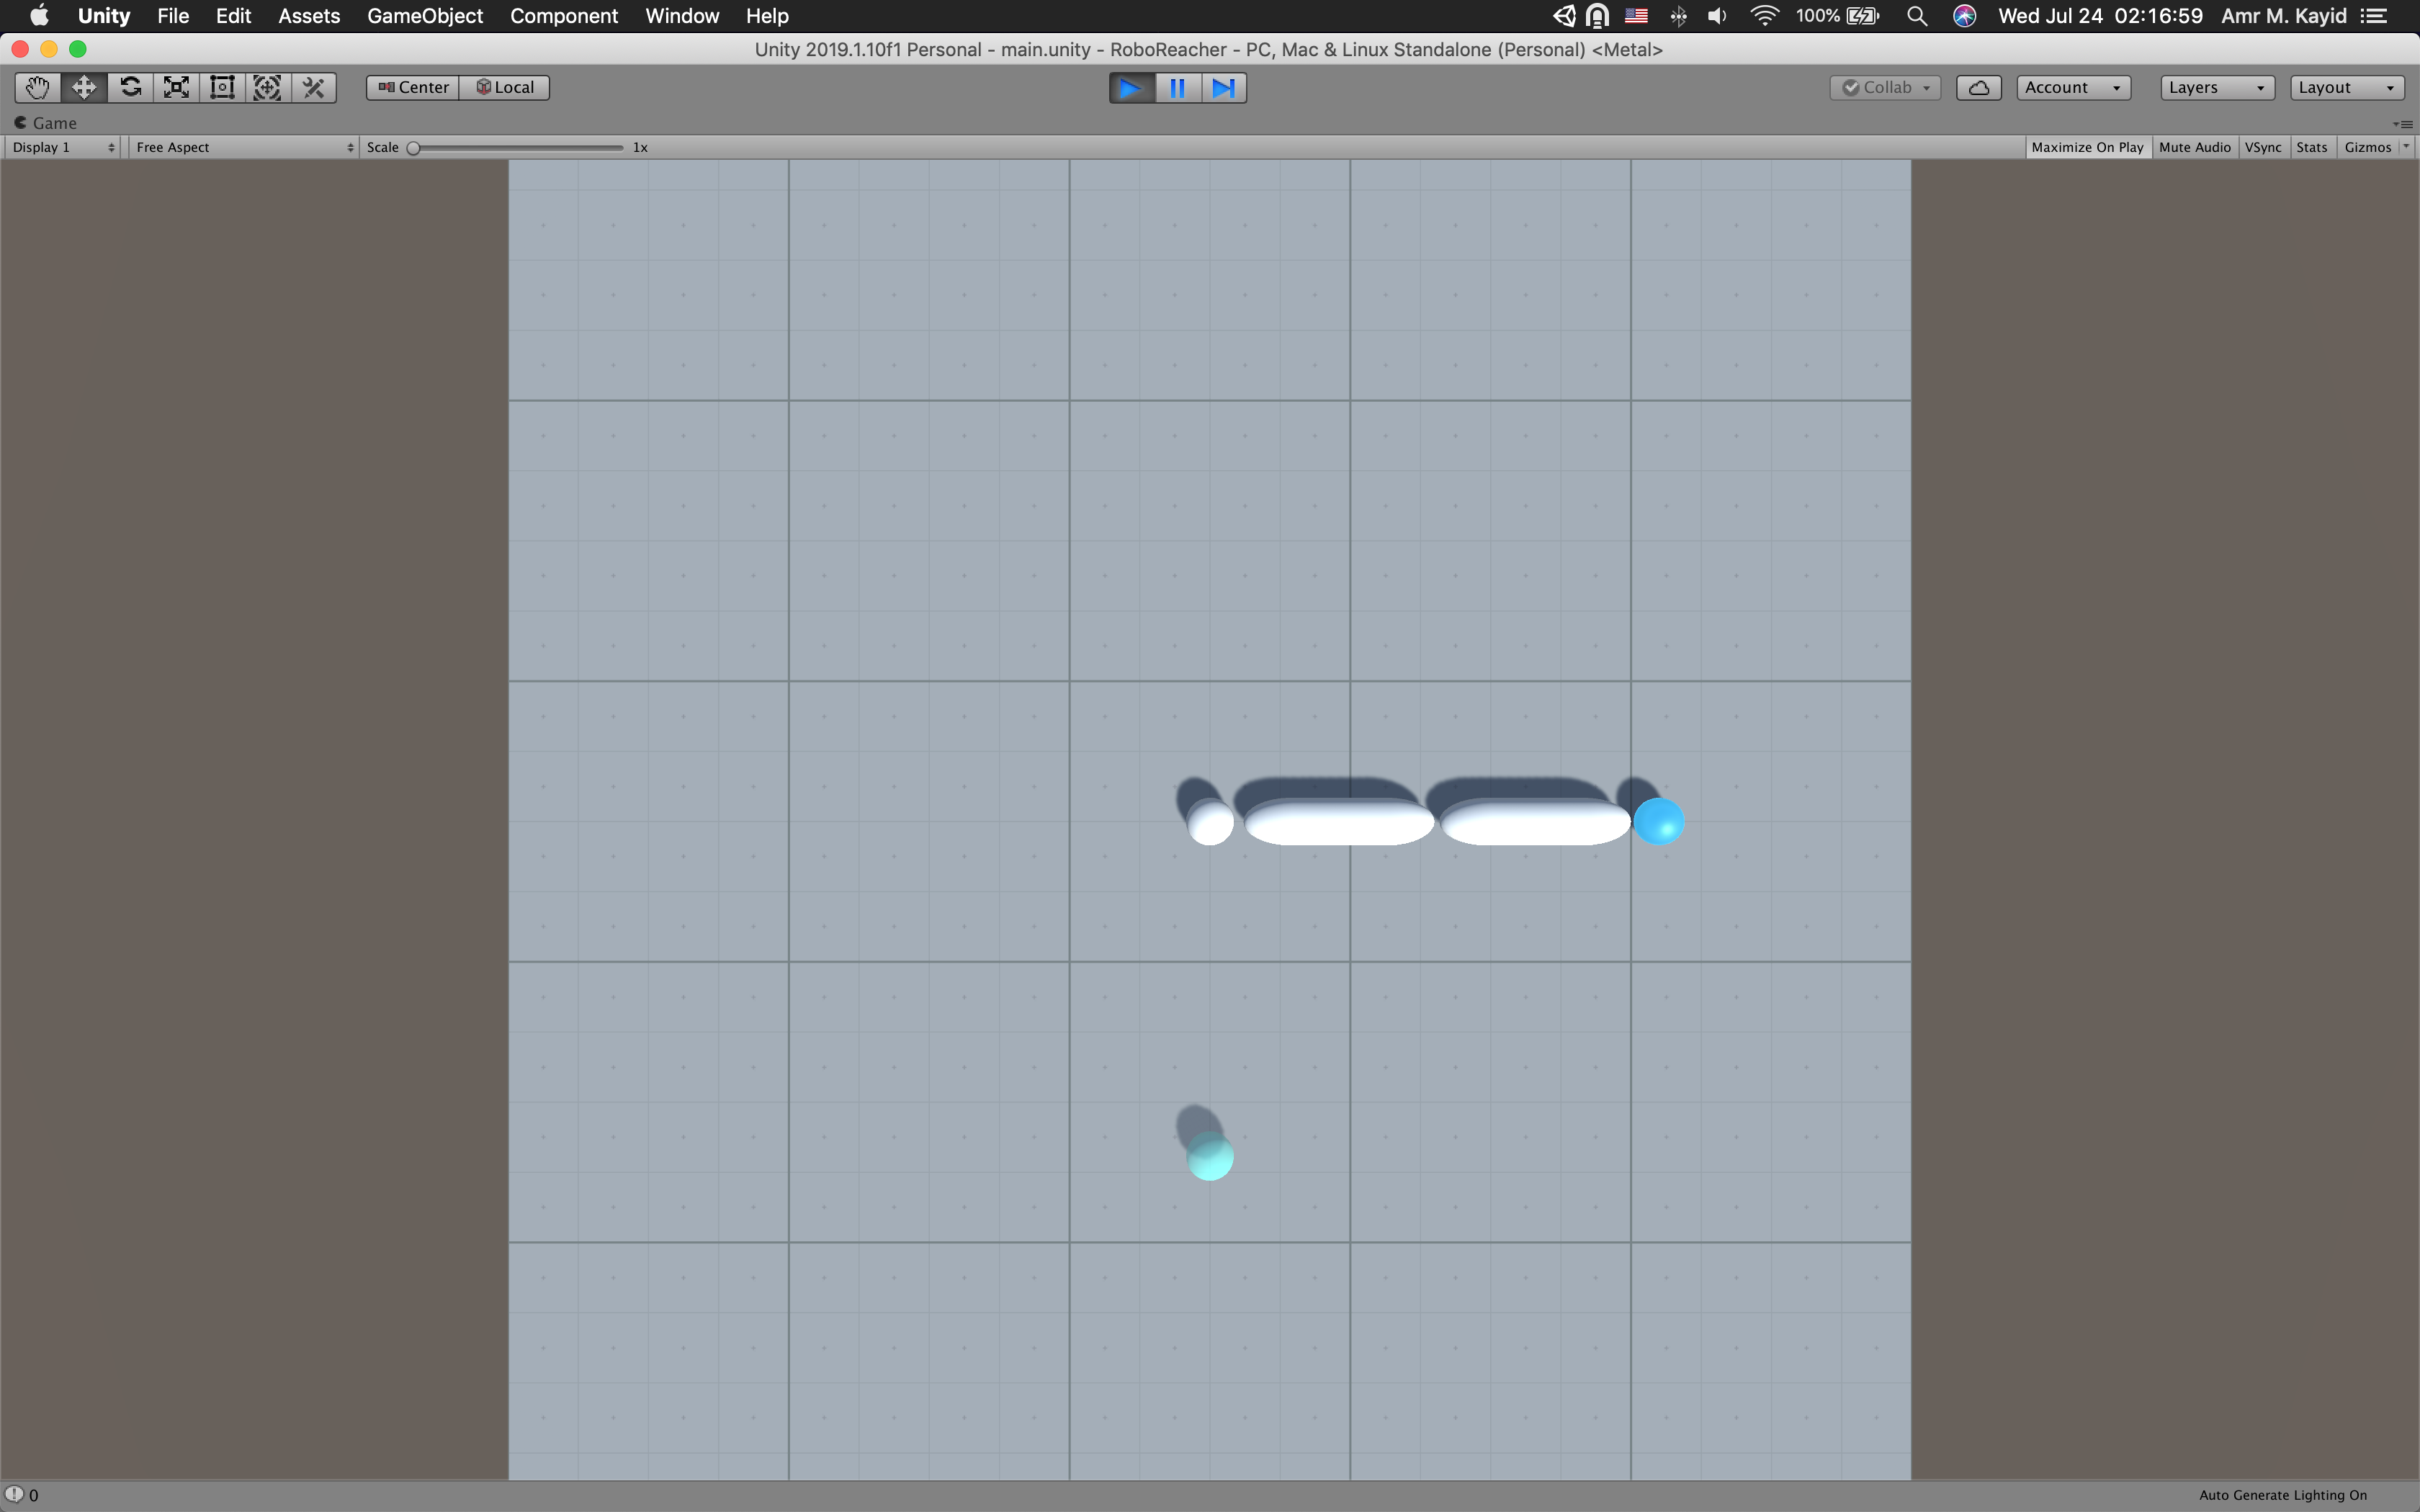
\includegraphics[width=0.7\linewidth]{figures/envs/unity_roboreacher.png}
            \caption{Replicated Gym Reacher Unity Environment}
            \label{fig:unity_reacher}
    \end{center}
\end{figure}


\textbf{Single Agent Reacher:} A robotic arm consist of two linked joints places in 3d plane surrounding it along with a moving sphere (target). The goal of the robotics arm it to reach target sphere and maintain following the point until the end of the episode. 

\begin{figure}[H]
    \begin{center}
            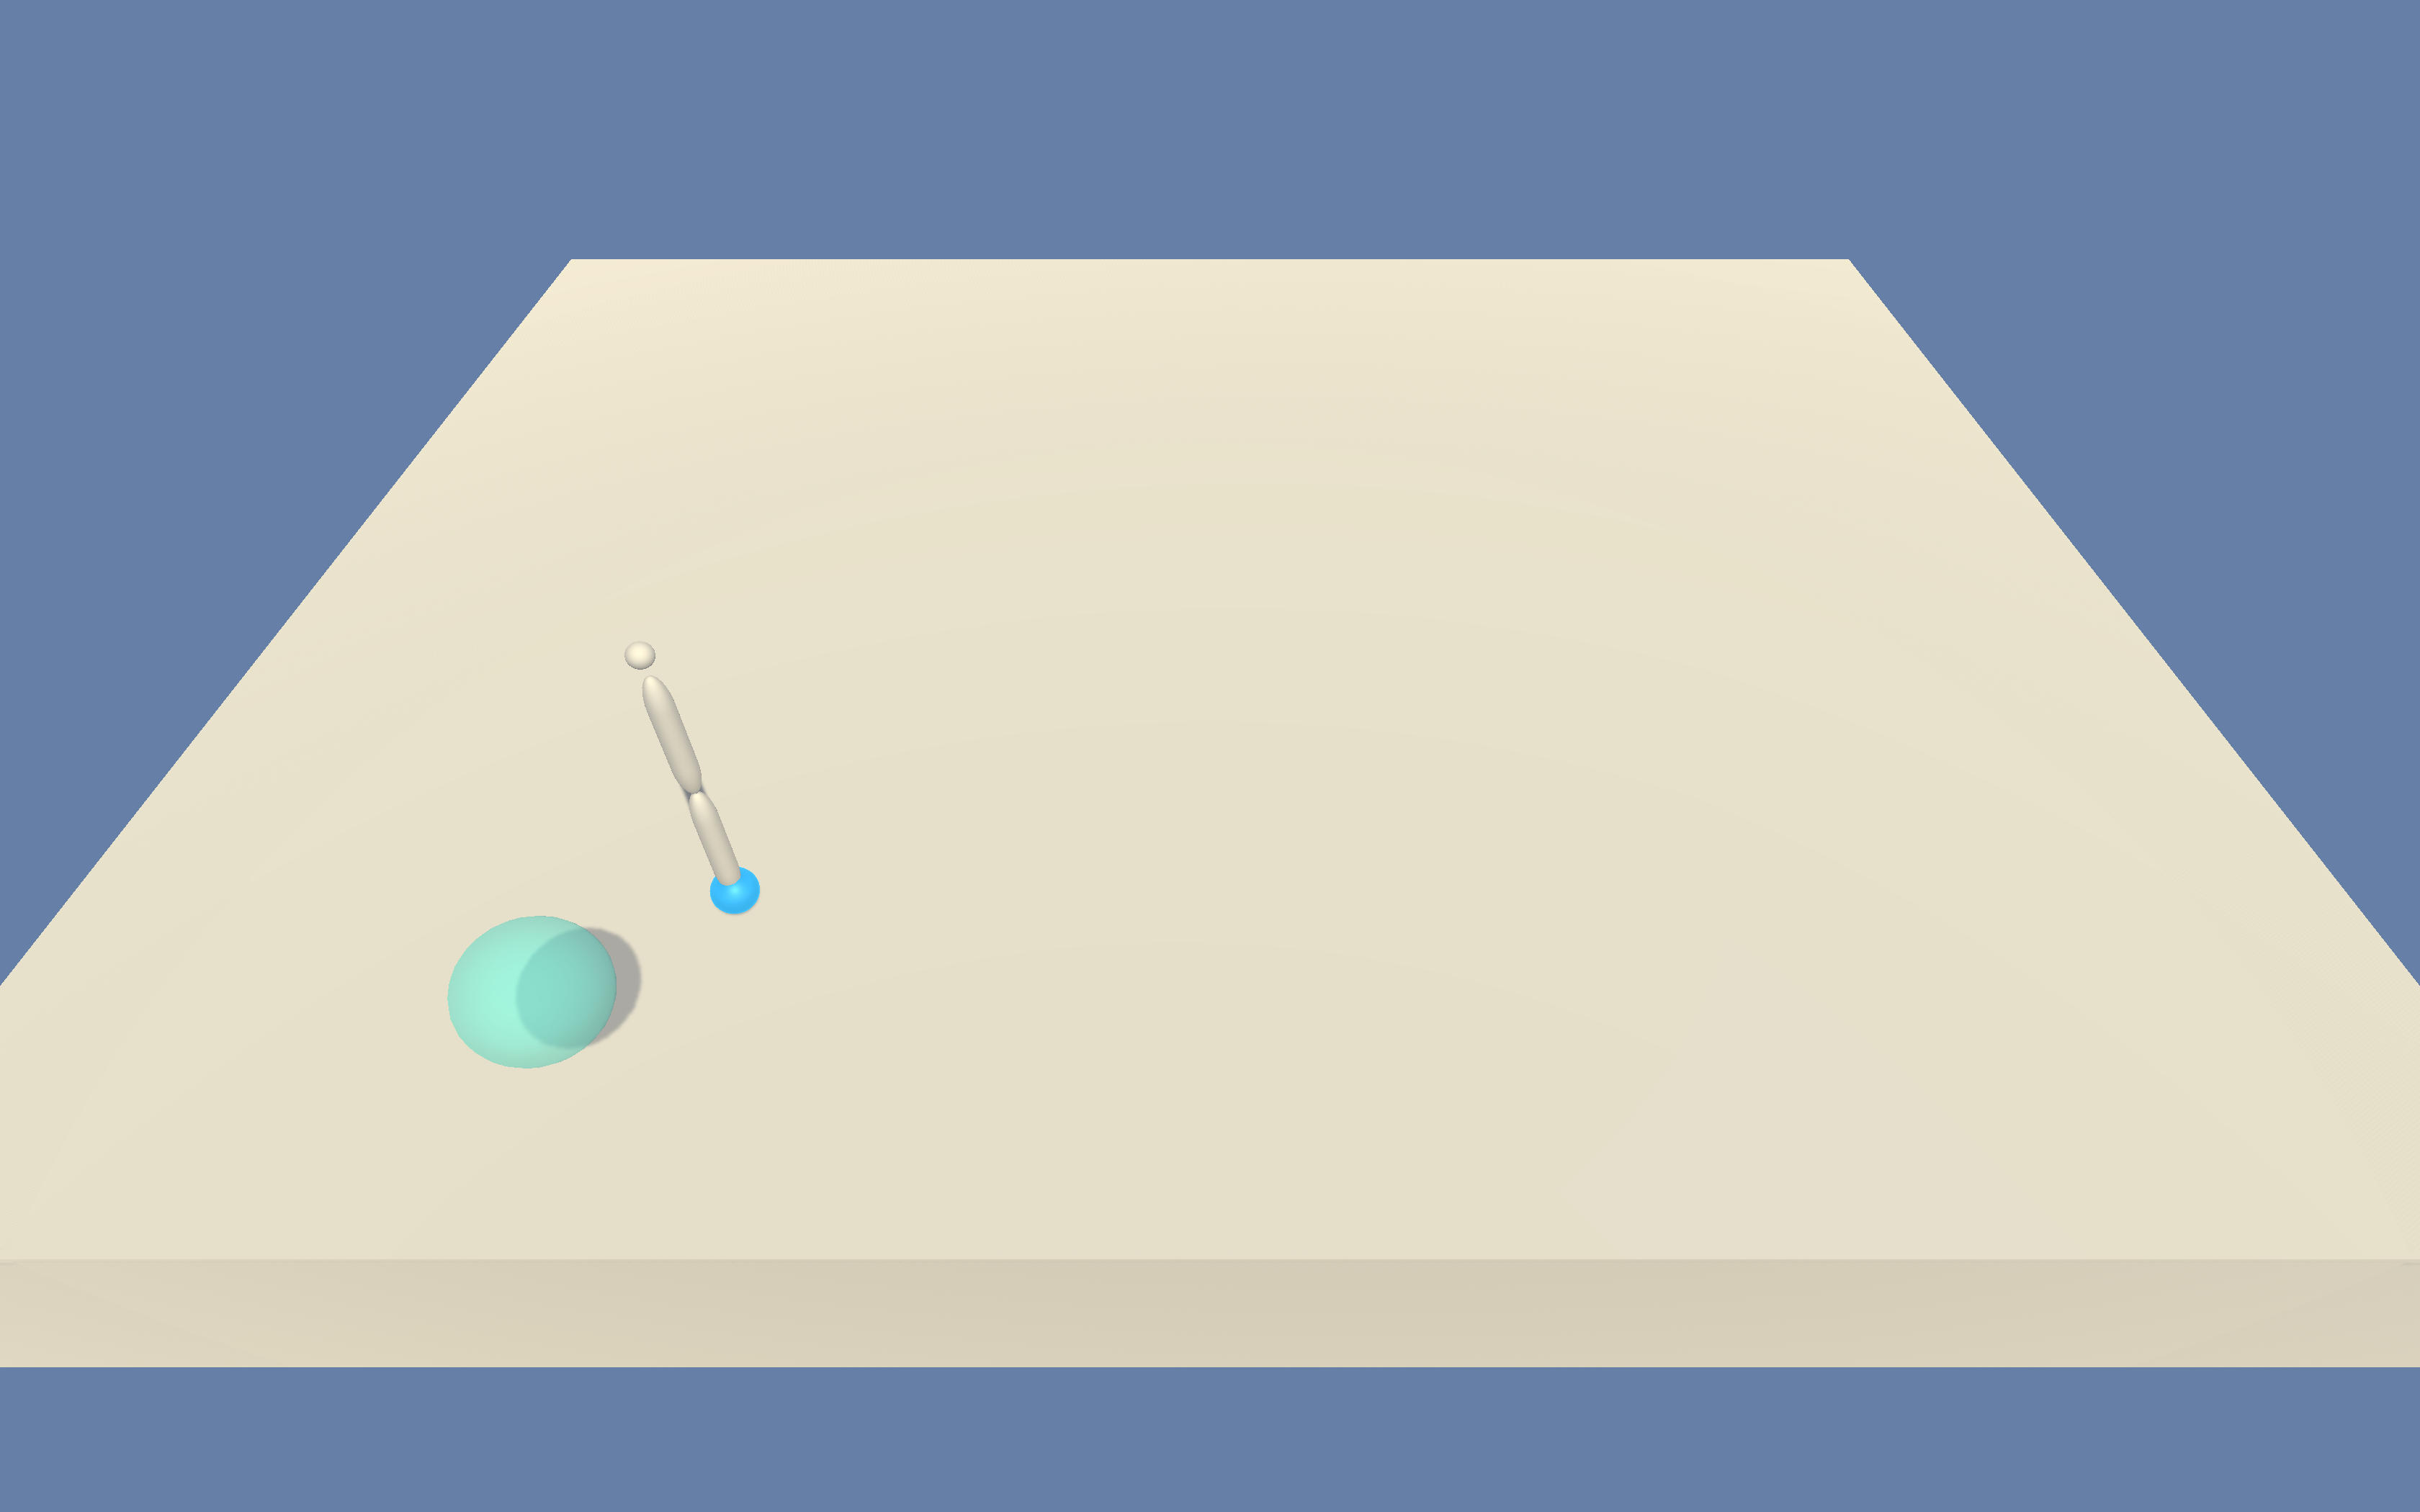
\includegraphics[width=0.7\linewidth]{figures/envs/unity_reacher_1.png}
            \caption{Unity Reacher Environment}
            \label{fig:unity_reacher_1}
    \end{center}
\end{figure}

\textbf{Multi-Agent Reacher:} in this environment, \textit{20 Agent} are used to parallelize the training process and collect more experiences and trajectories.

\begin{figure}[H]
    \begin{center}
            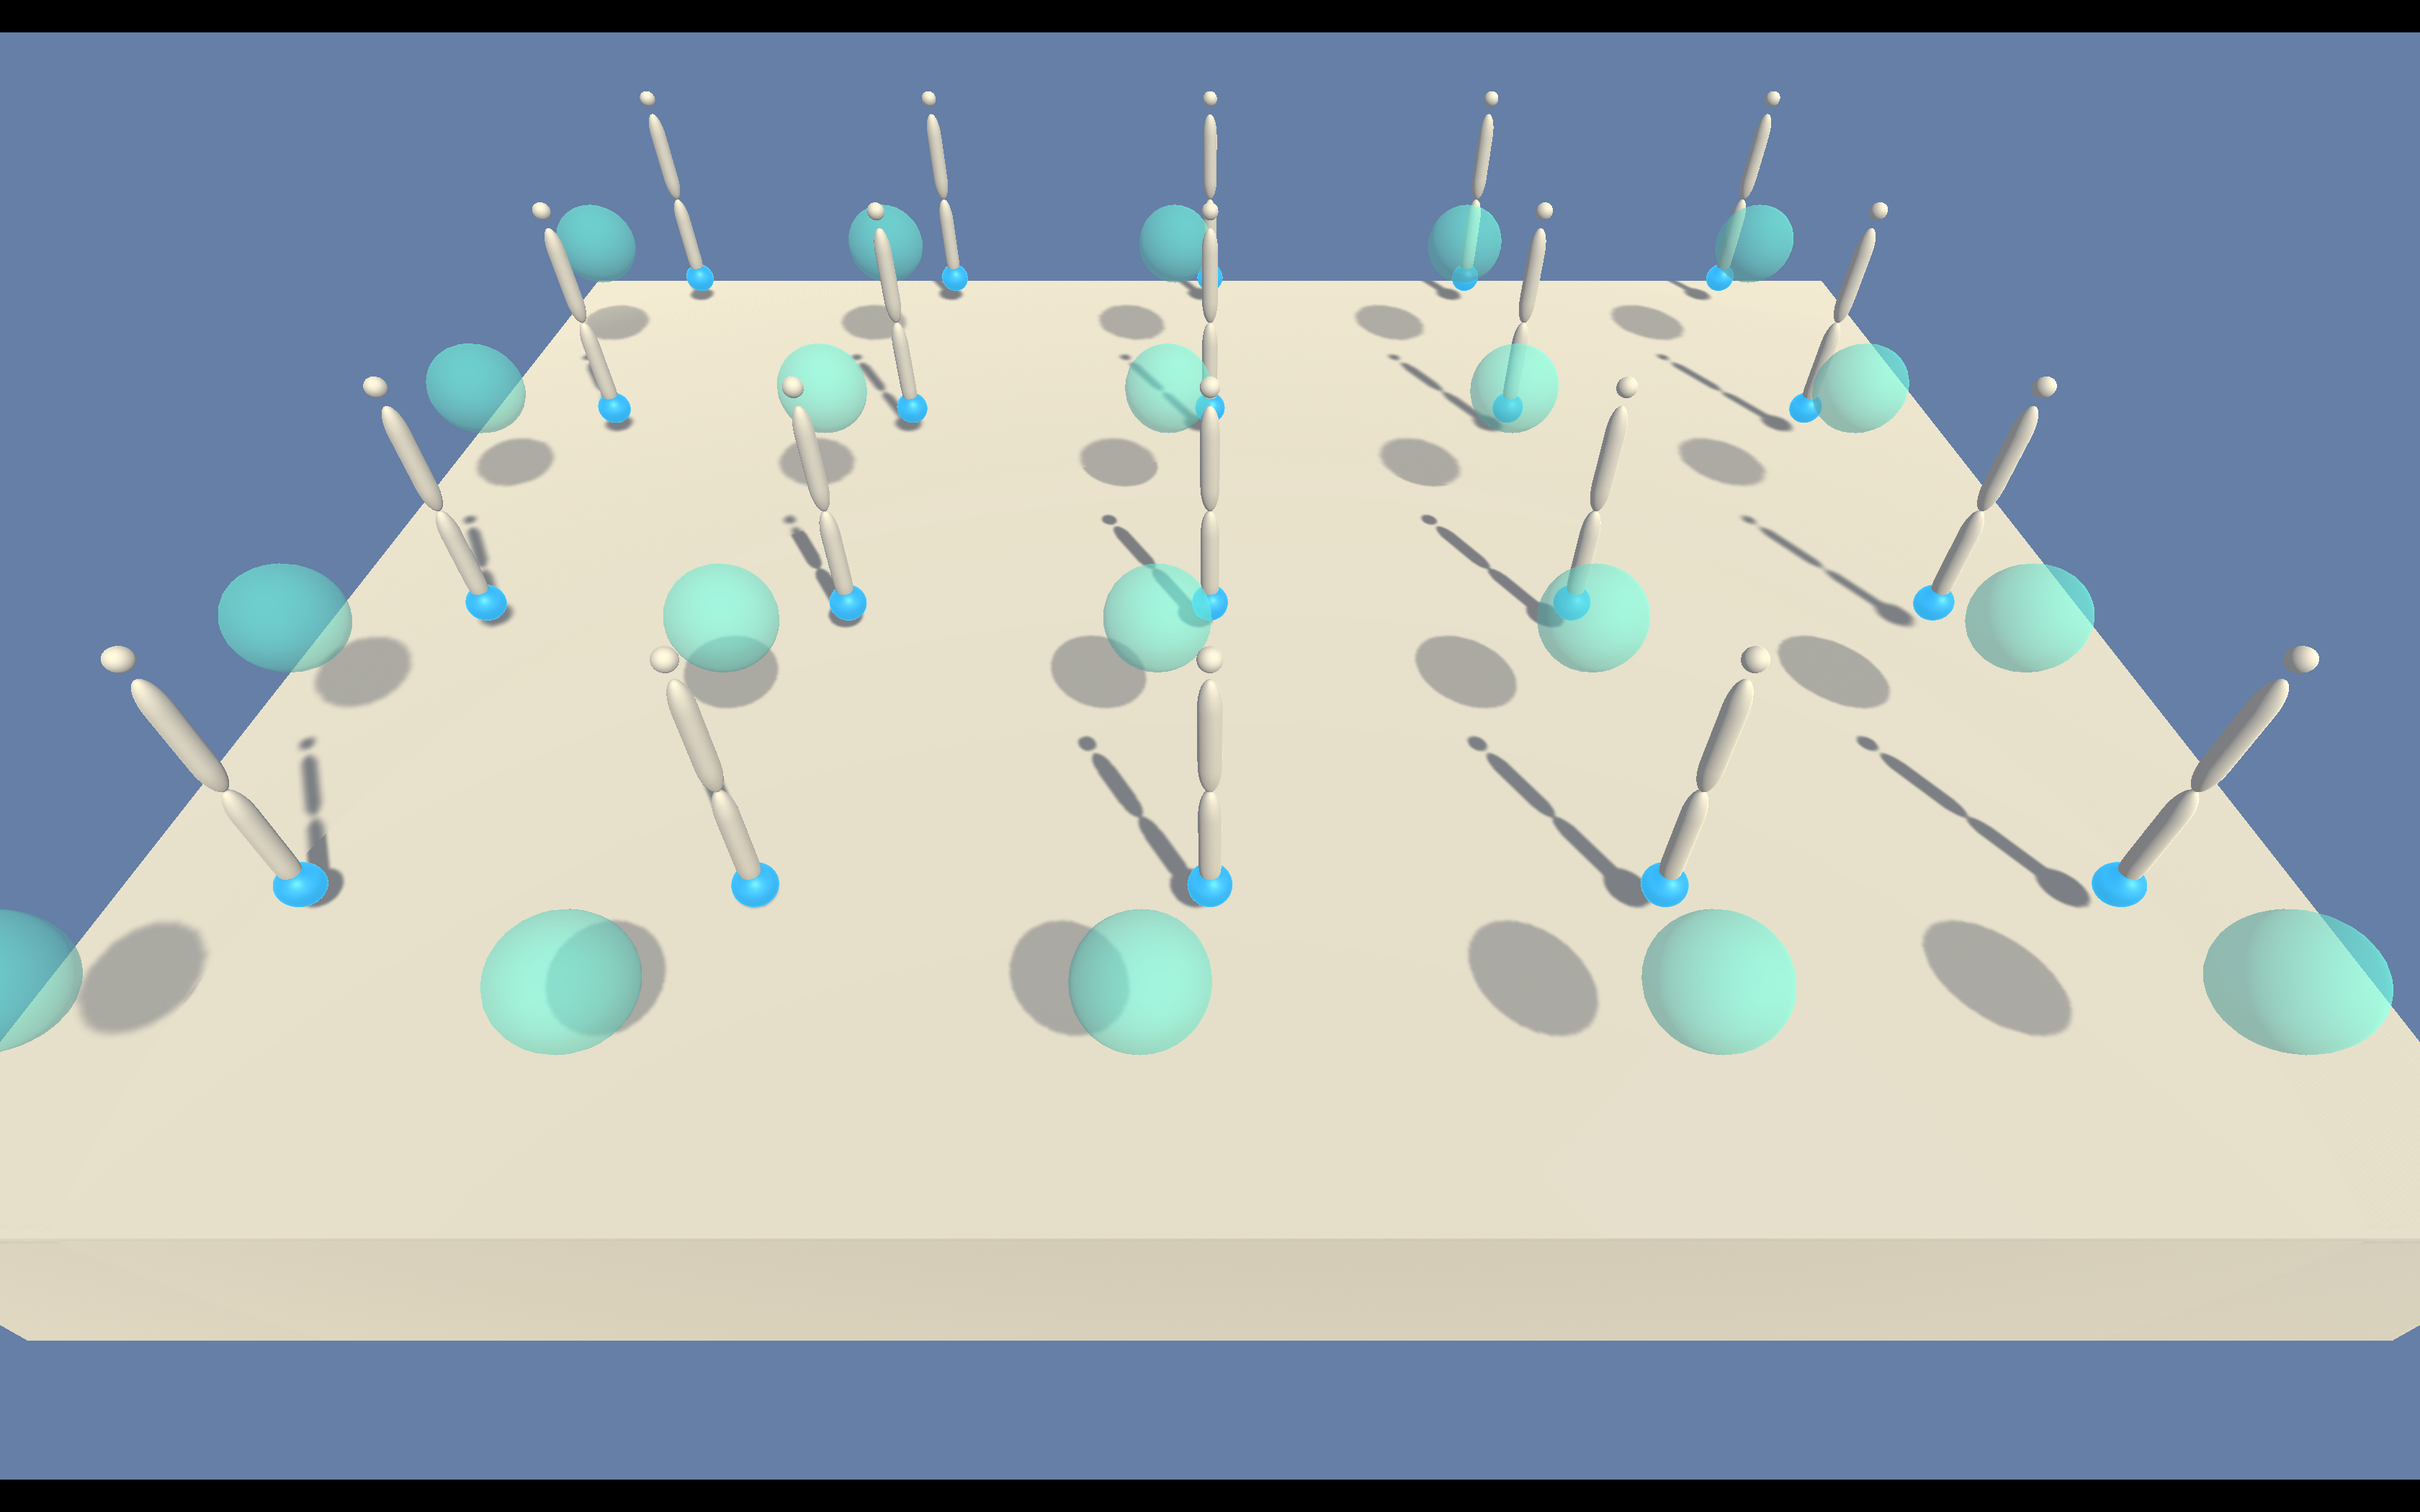
\includegraphics[width=0.7\linewidth]{figures/envs/unity_reacher_20.png}
            \caption{Unity Multi-Agent Reacher Environment}
            \label{fig:unity_reacher_20}
    \end{center}
\end{figure}

% !TeX root = ../../main.tex
% Add the above to each chapter to make compiling the PDF easier in some editors.

\chapter{Setup and Implementation}\label{chapter:setup_and_implementation}

In this chapter, the full details of the setups will be introduced. First, the used software framework will be presented. Then, our environments architecture and integration with the framework will be explained. Then, a brief description for the agents and algorithms will be shown. Lastly, description for all the used environments in our experiments will be provided.

\section{Overview}

Our approach is to setup a distributed learning architecture to run multiple experiments between selected environment and compare the results between training in normal non-distributed and distributed modes. We selected relatively close environment to robotics simulation with continuous observation and action spaces. A new abstract classes is introduced to run with the selected framework and unify the differences between different environments and physics simulators. A selection of the state of the art algorithms is used to train our reinforcement learning agents and compare between the algorithm and the modes for each algorithm.

\section{Software}
\textbf{Ray Framework~\parencite{moritz2018ray}: } Ray is a fast and simple framework for building and running distributed applications. The same code can be run on a single machine to achieve efficient multiprocessing, and it can be used on a cluster for large computations. Ray provide high scalability and a unified API for a variety of applications which is very useful for our experiments. Ray executes tasks asynchronously to achieve parallelism enabling us to run multiple environments in the same experiment to benefit from collection more experiences and trajectories for the agent.

\textbf{OpenAI Gym~\parencite{brockman2016openai}: } openai gym is a toolkit for developing and comparing reinforcement learning algorithms. It supports teaching agents everything from walking to playing games like Pong or Pinball. It has an open source interface to reinforcement learning tasks which provides an easy-to-use suite of reinforcement learning tasks. 

The core gym interface is \textbf{Env}, which is the unified environment interface. 
The following are the methods for the abstracted gym Env:

\begin{itemize}
    \item \textit{\textbf{\colorbox{gray!20}{reset(self)}}}: Reset the environment's state. Returns observation.
    \item \textit{\textbf{\colorbox{gray!20}{step(self, action)}}}: Step the environment by one time-step. Returns observation, reward, done, info.
    \item \textit{\textbf{\colorbox{gray!20}{render(self, mode='human')}}}: Render one frame of the environment. The default mode will do something human friendly, such as pop up a window.
\end{itemize}

\textbf{Unity MLAgents~\parencite{juliani2018unity}: } unity mlagents toolkit is an open-source Unity plugin that enables games and simulations to serve as environments for training intelligent agents. It has more realistic and complex simulation environments. It provides the ability to flexibly configure
the simulation. By taking advantage of Unity as a simulation platform, the toolkit enables the development of learning environments which are rich in sensory and physical complexity, provide compelling cognitive challenges, and support dynamic multi-agent interaction. Agents can be trained using reinforcement learning, imitation learning, neuroevolution, or other machine learning methods through a simple-to-use Python API. They provide implementations of state-of-the-art algorithms to enable game developers and hobbyists to easily train intelligent agents for 2D, 3D and VR/AR games. We are using this to test running multiple agents in the same environment and compare the effect with one agent only. Also, to experiment the transferability between different physics simulators.

\section{Architecture}

At a high level, ray provides an \textbf{\colorbox{gray!20}{Trainer}} class which holds a policy for environment interaction. Through the trainer interface~\ref{fig:ray_trainer}, the policy can be trained, check-pointed, or an action computed. In multi-agent training, the trainer manages the querying and optimization of multiple policies at once. It provides custom resources configurations~\ref{fig:ray_config}, which can control the degree of parallelism used by setting the \colorbox{gray!20}{\texttt{num\_workers}} hyper-parameter for most algorithms. The number of GPUs the driver should use can be set via the \colorbox{gray!20}{\texttt{num\_gpus}} option. Similarly, the resource allocation to workers can be controlled via \colorbox{gray!20}{\texttt{num\_cpus\_per\_worker}}, \colorbox{gray!20}{\texttt{num\_gpus\_per\_worker}}, and \colorbox{gray!20}{\texttt{custom\_resources\_per\_worker}}. The number of GPUs can be a fractional quantity to allocate only a fraction of a GPU. For example, with DQN you can pack five trainers onto one GPU by setting \colorbox{gray!20}{\texttt{num\_gpus}: 0.2}.

\begin{figure}[H]
	\centering
	\begin{subfigure}[b]{0.4\textwidth}
		\centering
		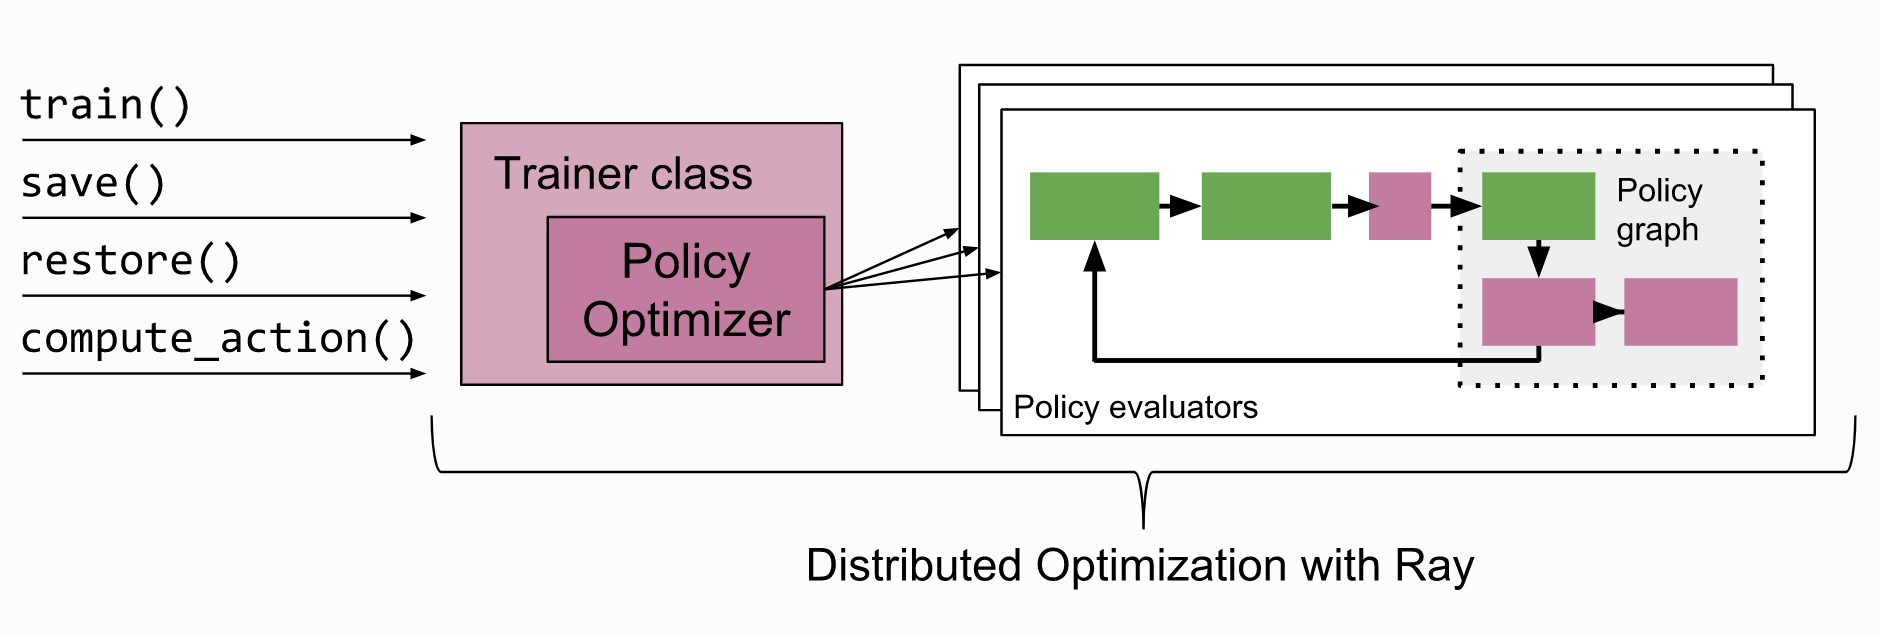
\includegraphics[width=\textwidth]{figures/architecture/ray_trainer.png}
		\caption{Ray Training Process}
		\label{fig:ray_trainer}
    \end{subfigure}
    \hfill
	\begin{subfigure}[b]{0.4\textwidth}
		\centering
		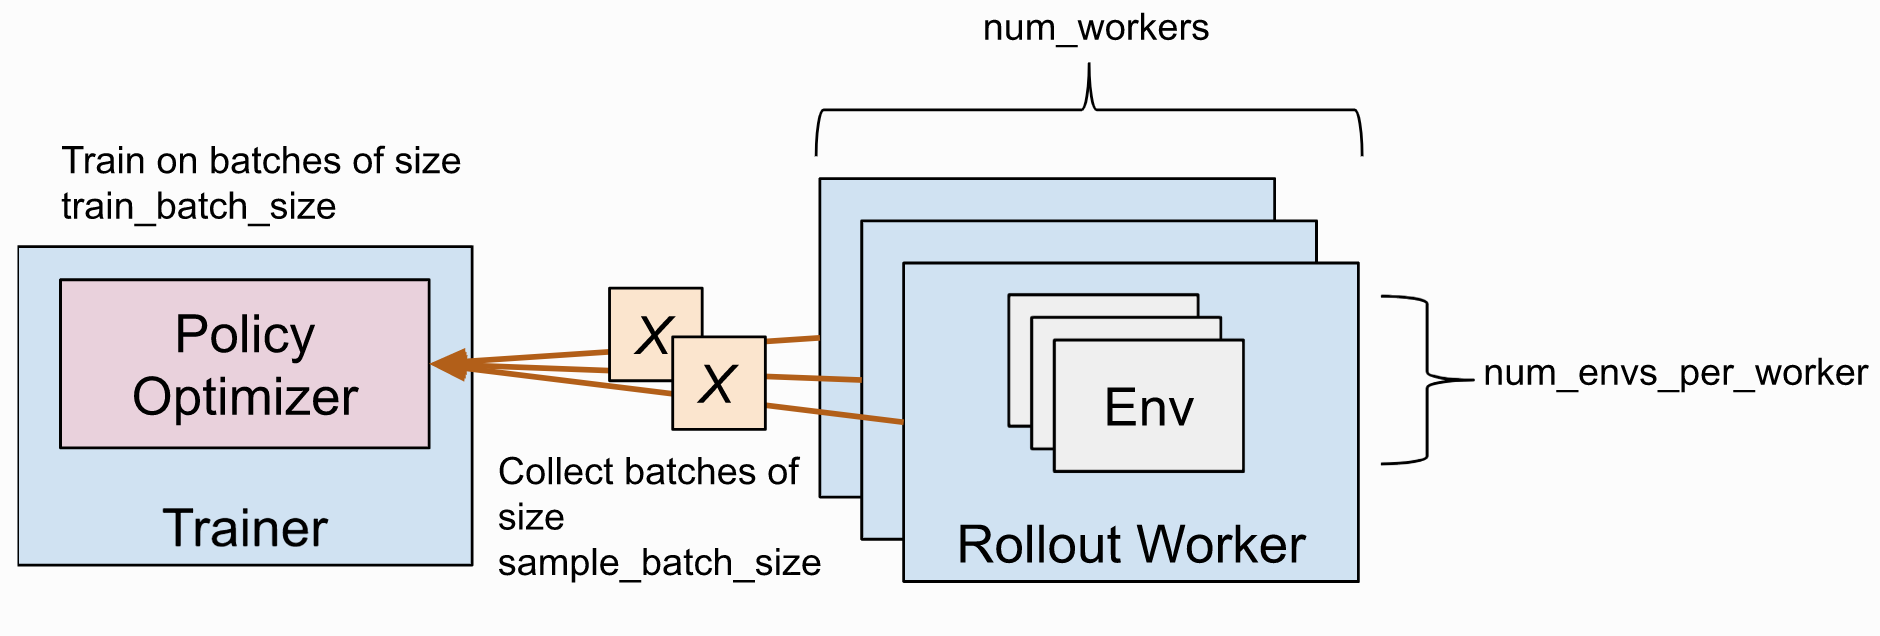
\includegraphics[width=\textwidth]{figures/architecture/ray_config.png}
        \caption{Ray Configurable resources}
		\label{fig:ray_config}
	\end{subfigure}
	\hfill
	   \caption{General Overview of Ray framework~\parencite{moritz2018ray}}
	   \label{fig:ray}
\end{figure}

Since ray support only OpenAI Gym environments along with their provided multi-agent and also batched environments, we had to implement our custom environment to unify between unity mlagents and openai gym environments. Also, we implemented our custom Multi-Agent environments for both used environments as shown in the following figure~\ref{fig:ray_envs}.

\begin{figure}[H]
	\centering
		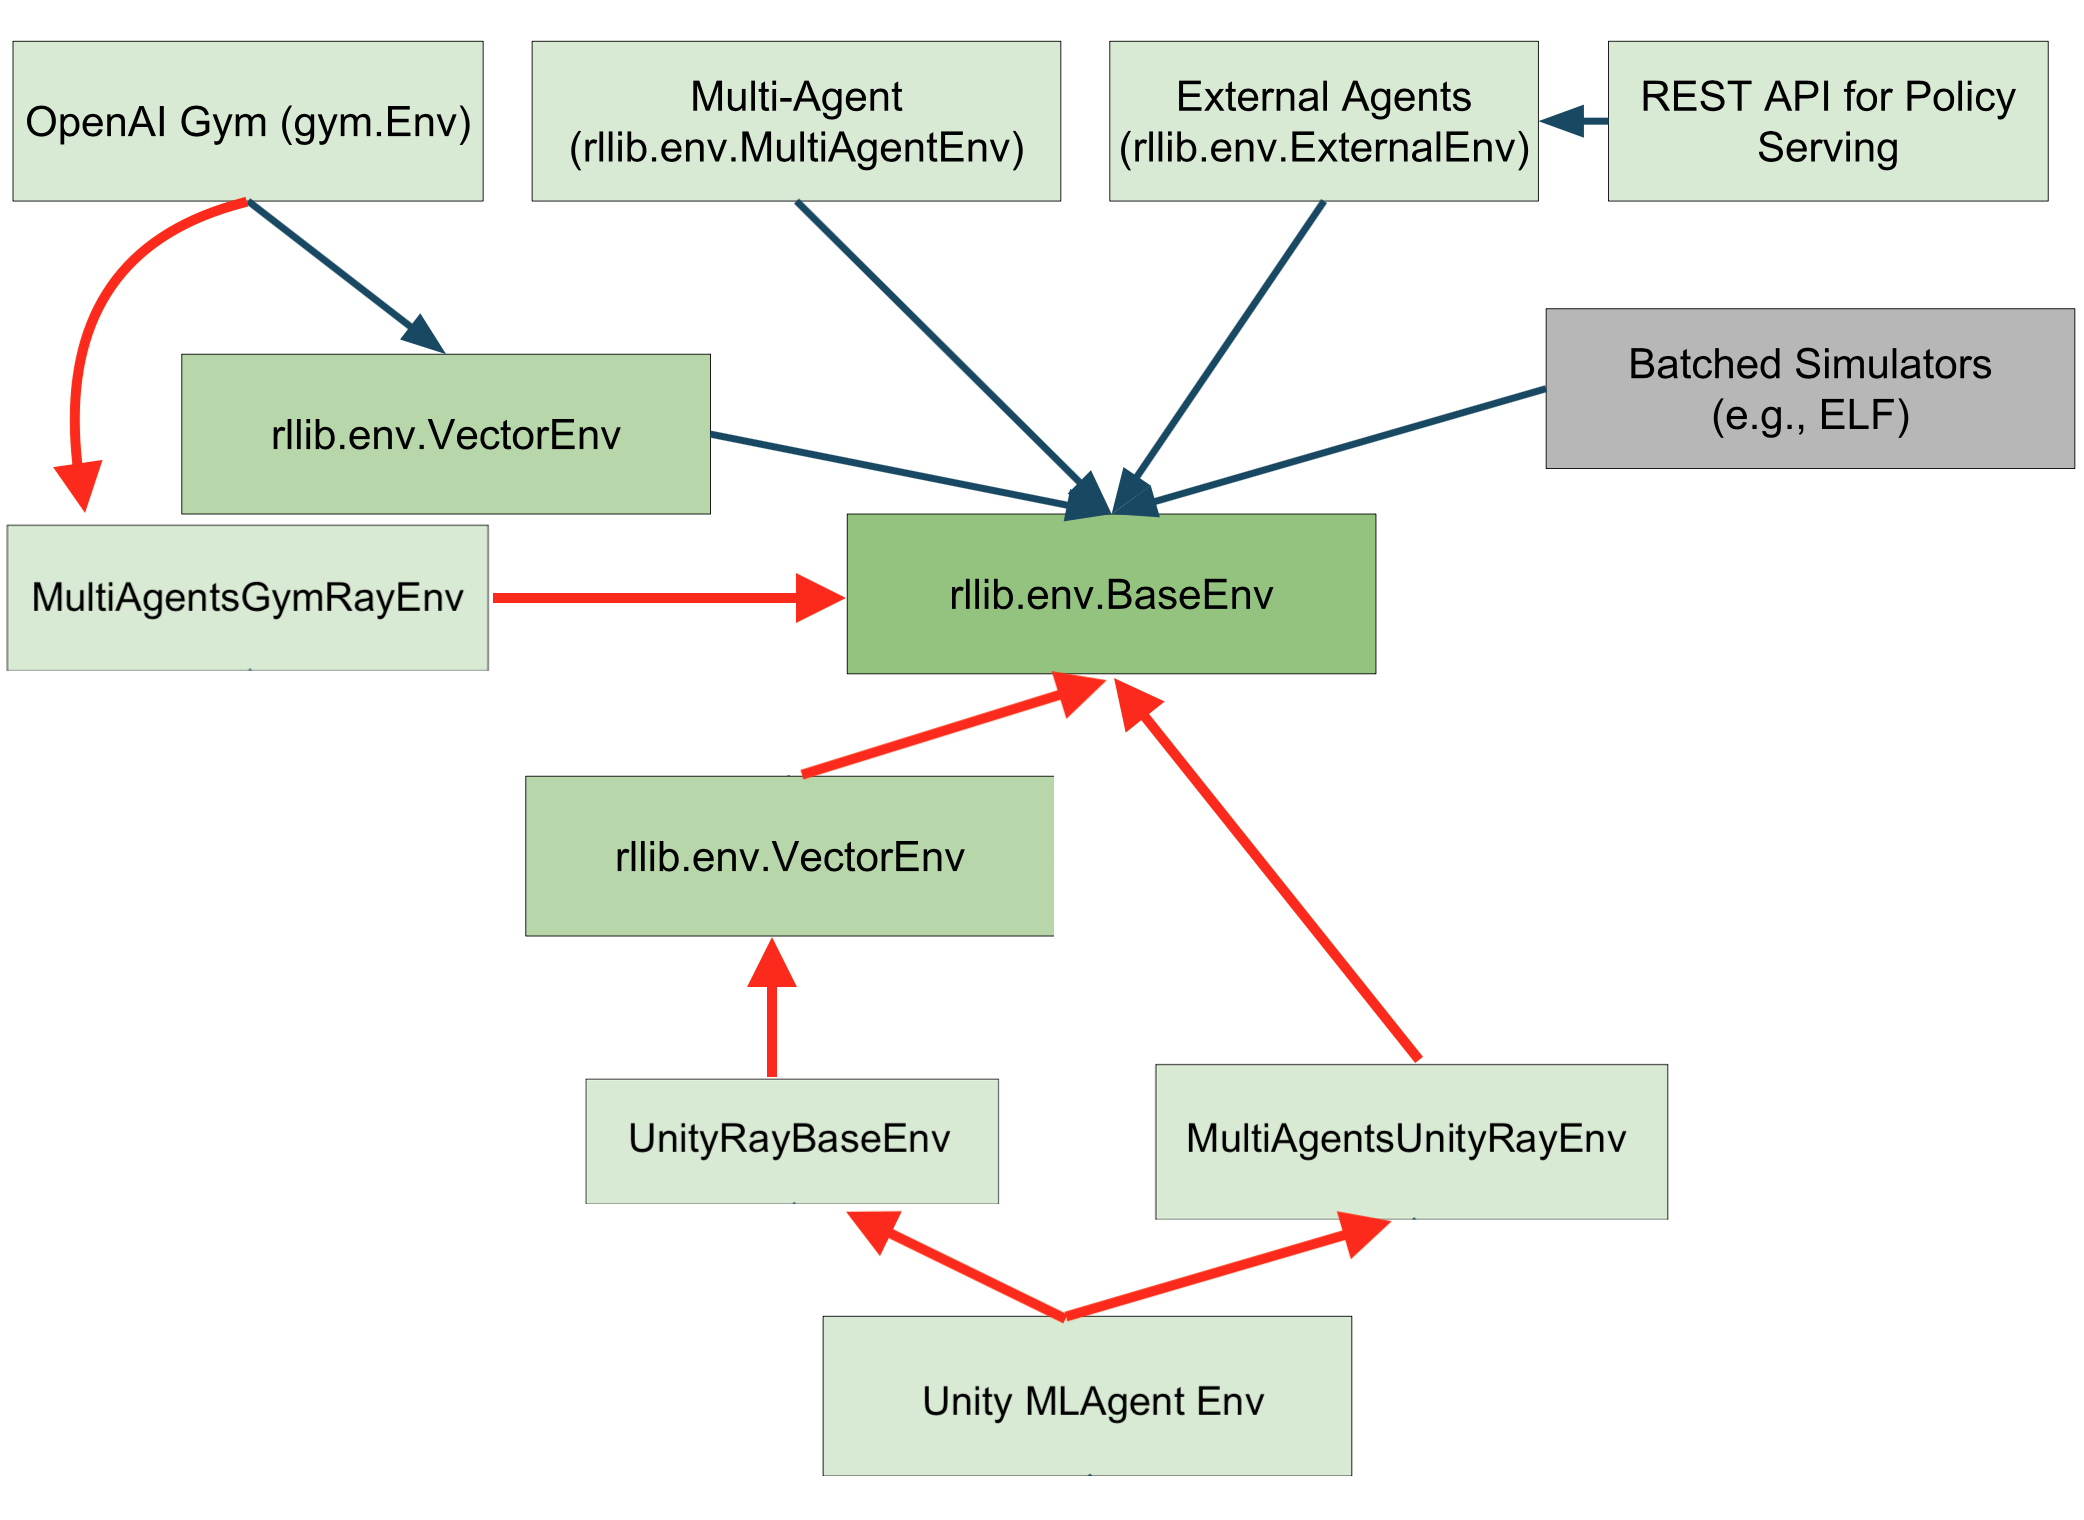
\includegraphics[width=\linewidth]{figures/architecture/ray_envs.png}
		\caption{Our Custom Environments}
		\label{fig:ray_envs}
\end{figure}

\clearpage

Custom environments implementations and methods are described below:

\textbf{UnityRayEnv}:\\
our base unity environment maps the observations and actions from unity mlagents toolkit to be compatible with Ray BaseEnv. Since unity mlagents deals with brains that control the agents and the environments we had to convert it to the required \colorbox{gray!20}{\texttt{observation\_space}} and \colorbox{gray!20}{\texttt{action\_space}} for ray env with the following methods:
\begin{itemize}
    \item \textit{\textbf{\colorbox{gray!20}{\texttt{\_\_init\_\_(self)}}}}: Create the unity environment from the unity build env, convert the observation and action spaces to be ray-compatible.
    \item \textit{\textbf{\colorbox{gray!20}{reset(self)}}}: Reset the environment's state. Returns observation.
    \item \textit{\textbf{\colorbox{gray!20}{step(self, action)}}}: Step the environment by one time-step. Returns observation, reward, done, info.
\end{itemize}

\textbf{MultiAgentsUnityRayEnv}:\\
this class inherit from both \colorbox{gray!20}{\textbf{UnityRayEnv}} and \colorbox{gray!20}{\textbf{MultiAgentEnv}}~\ref{fig:ray_multiagentenv}. The difference from the base environment is in both methods \textit{\textbf{\colorbox{gray!20}{reset(self)}}} and \textit{\textbf{\colorbox{gray!20}{step(self, \texttt{actions\_dict})}}}, where the reset function reset all the observations for each agent that exist in the environment and step function take a dictionary of actions corresponding for each action of a single agent. The same applies to \textbf{MultiAgentsGymRayEnv}.

\begin{figure}[H]
	\centering
		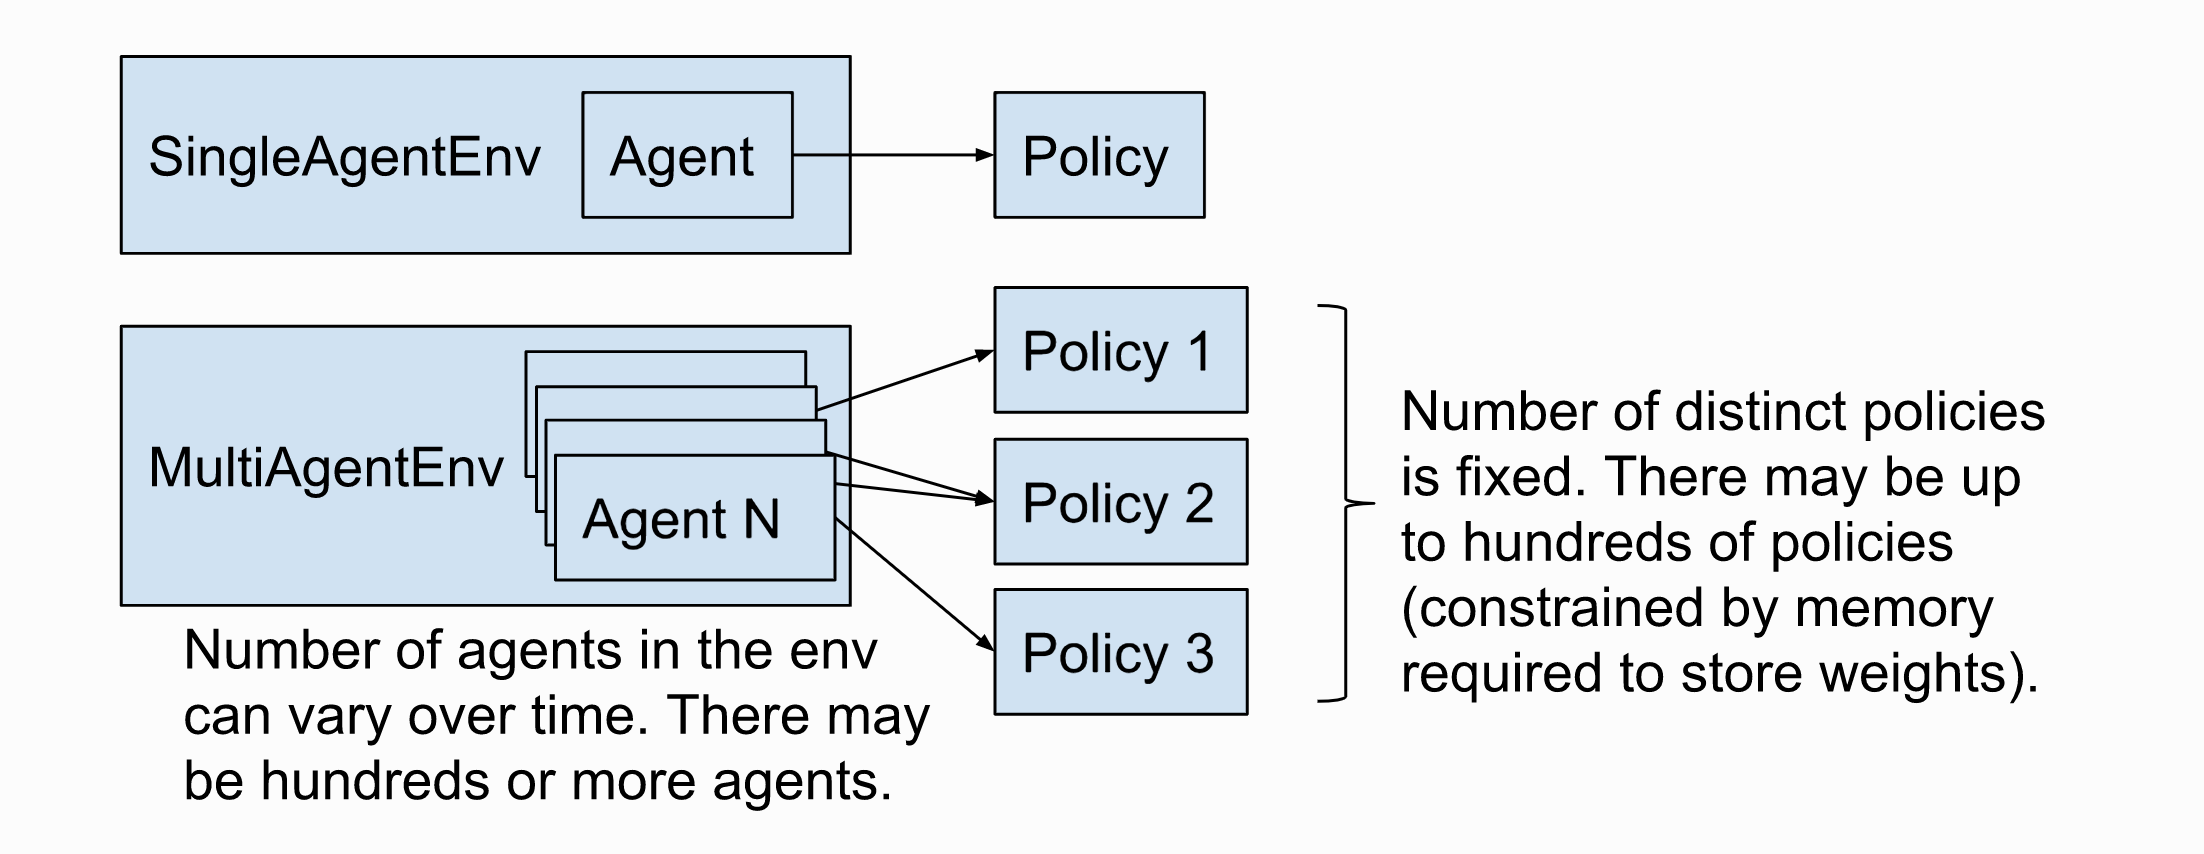
\includegraphics[width=\linewidth]{figures/architecture/ray_multiagentenv.png}
		\caption{Ray MultiAgentEnv}
		\label{fig:ray_multiagentenv}
\end{figure}

\section{Agents and Algorithms}

\begin{itemize}
    \item \textbf{Proximal Policy Optimization (PPO)}: PPO’s clipped objective supports multiple SGD passes over the same batch of experiences. RLlib’s multi-GPU optimizer pins that data in GPU memory to avoid unnecessary transfers from host memory, substantially improving performance over a naive implementation. RLlib’s PPO scales out using multiple workers for experience collection, and also with multiple GPUs for SGD.

    \item \textbf{Distributed Prioritized Experience Replay (Ape-X)}: Ape-X variations of DQN, DDPG, use a single GPU learner and many CPU workers for experience collection. Experience collection can scale to hundreds of CPU workers due to the distributed prioritization of experience prior to storage in replay buffers.

    \item \textbf{Importance Weighted Actor-Learner Architecture (IMPALA)}: In IMPALA, a central learner runs SGD in a tight loop while asynchronously pulling sample batches from many actor processes. RLlib’s IMPALA implementation uses DeepMind’s reference V-trace code. Note that we do not provide a deep residual network out of the box, but one can be plugged in as a custom model. Multiple learner GPUs and experience replay are also supported.
\end{itemize}

\section{Environments and Tasks Description}
Our task is robotic related task, where we have a robotic arm consist of two linked joints \textit{(agent)} and moving sphere \textit{(target)}. The robotic arm and the goal differ according to the environment used. We have a one experiment where is the agent movement is in 2D and the goal of the agent it to reach the target as fast as possible to maximize the given cumulative reward. In the second experiment, the agent can move in 3D and the goal is to keep track of the moving target and move with it along the 3D space.

Following is detailed description for all the environment used in our experiments.

\textbf{OpenAI: Reacher Environment}

Our first and baseline environment is \textit{Reacher Environment}~\ref{fig:openai_reacher}: A robotic arm consist of two linked joints places in a squared arena surrounding it along with a moving sphere (target). The goal of the robotics arm it to reach target sphere and maintain following the point until the end of the episode. 

\begin{figure}[H]
    \begin{center}
            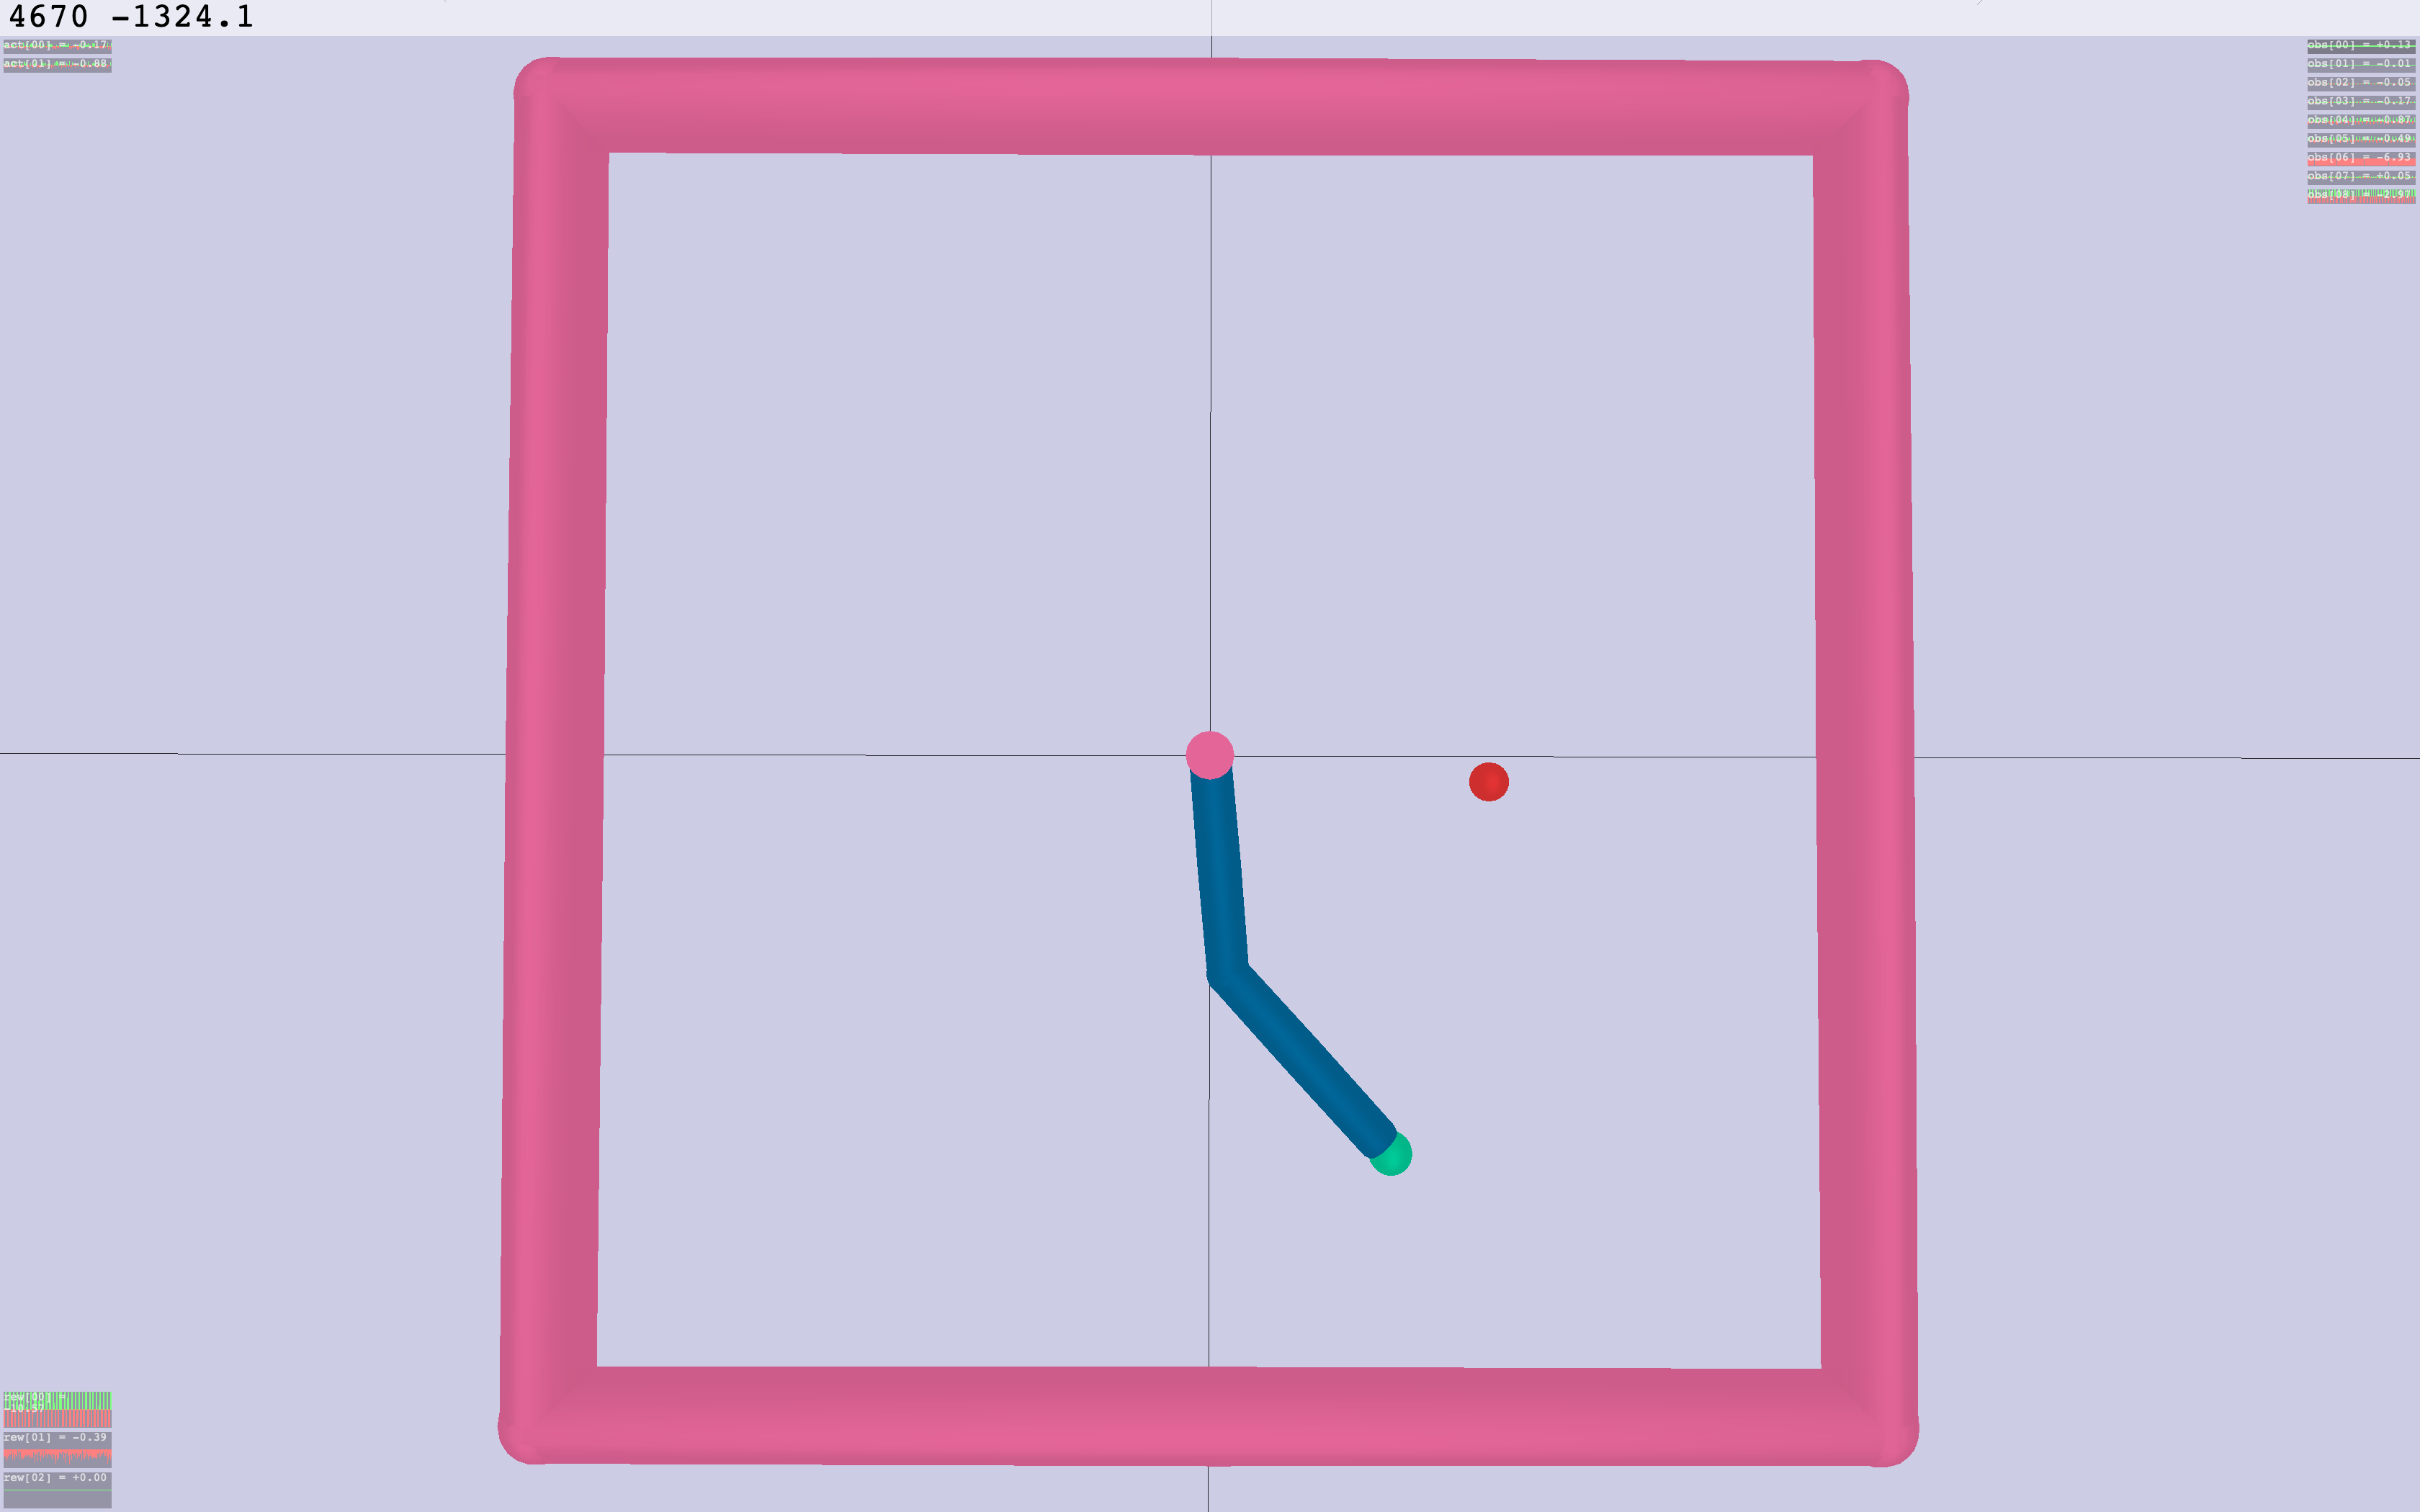
\includegraphics[width=0.7\linewidth]{figures/envs/openai_roboreacher.png}
            \caption{OpenAI Reacher Environment}
            \label{fig:openai_reacher}
    \end{center}
\end{figure}

\begin{table}[!htb]
    \centering
    \begin{subtable}{.4\linewidth}
        \centering
        \begin{tabular}{|c|c|}
        \hline
        \multicolumn{2}{|c|}{{\ul \textit{\textbf{Observation Space}}}}                                                                                   \\ \hline
        \multirow{2}{*}{\textbf{Target Position}}                                                                      & \textit{X Position}              \\ \cline{2-2} 
                                                                                                                    & \textit{Y Position}              \\ \hline
        \multirow{2}{*}{\textbf{Arm to Target Vector}}                                                                 & \textit{Position vector 0}       \\ \cline{2-2} 
                                                                                                                    & \textit{Position vector 1}       \\ \hline
        \multirow{2}{*}{\textbf{\begin{tabular}[c]{@{}c@{}}Current Relative Position\\ of Central Joint\end{tabular}}} & \textit{cosine of central joint} \\ \cline{2-2} 
                                                                                                                    & \textit{sine of central joint}   \\ \hline
        \multirow{2}{*}{\textbf{\begin{tabular}[c]{@{}c@{}}Current Relative Position\\ of Elbow Joint\end{tabular}}}   & \textit{cosine of elbow joint}   \\ \cline{2-2} 
                                                                                                                    & \textit{sine of elbow joint}     \\ \hline
        \end{tabular}
        \caption{Gym Reacher Observation Information}
        \label{tab:gym_reacher_obs}
    \end{subtable}%
    \hfill
    \begin{subtable}{.4\linewidth}
        \centering
        \begin{tabular}{|c|c|}
            \hline
            \multicolumn{2}{|c|}{{\ul \textit{\textbf{Action Space (Continuous)}}}}                             \\ \hline
            \multirow{2}{*}{\textbf{Center Joint Torque}} & \multirow{2}{*}{\textit{range(-1, 1)}} \\
                                                          &                                        \\ \hline
            \multirow{2}{*}{\textbf{Elbow Joint Torque}}  & \multirow{2}{*}{\textit{range(-1, 1)}} \\
                                                          &                                        \\ \hline
            \end{tabular}
            \caption{Gym Reacher Action Information}
            \label{tab:gym_reacher_actions}
    \end{subtable}%
    \caption{Gym Reacher Observation and Action Information}
\end{table}

the reward function is designed based on the distance between the arm and the target along with electricity cost of the torque and angular velocity of the arm with small epsilon amount in case of the joint is stuck. 

\clearpage

\textbf{Unity MLAgents: 2D and 3D Reacher Environment}

We have replicate the same openai gym reacher environment in unity to test the transferability between different physics engines, along with two 3d reacher environment (single and multi-agents) described below:

\textbf{Replicated Gym Env:}

\begin{figure}[H]
    \begin{center}
            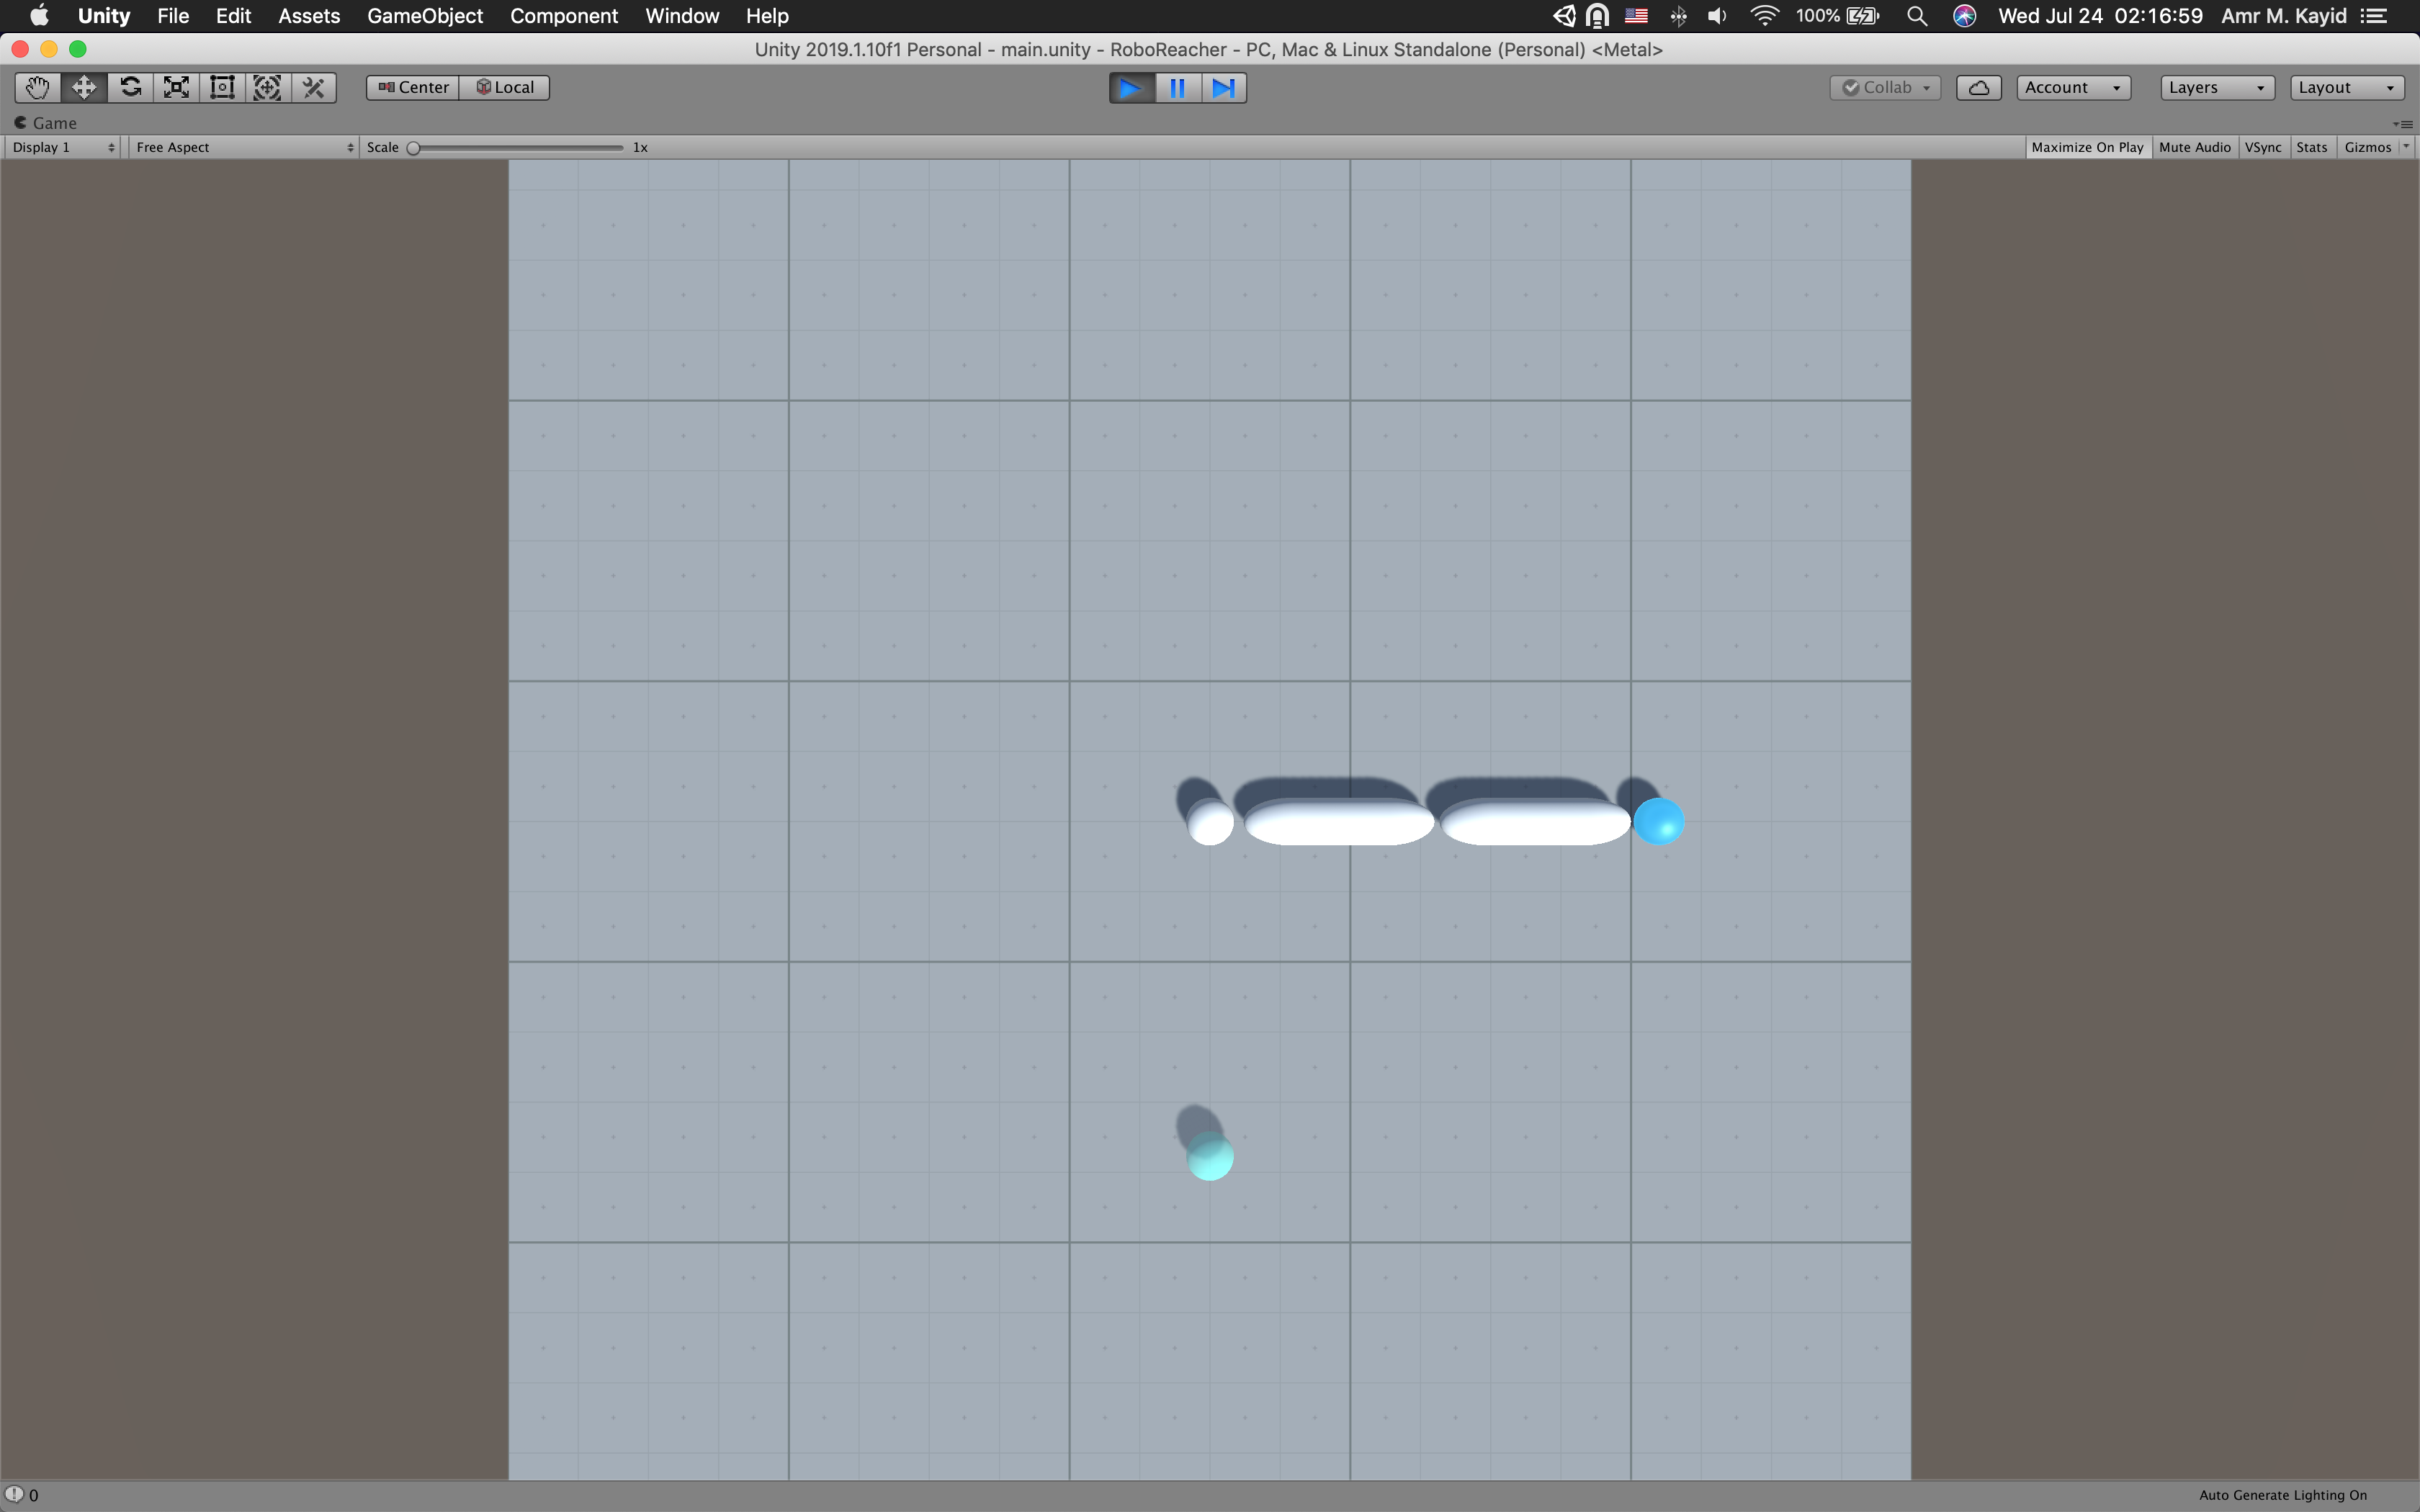
\includegraphics[width=0.7\linewidth]{figures/envs/unity_roboreacher.png}
            \caption{Replicated Gym Reacher Unity Environment}
            \label{fig:unity_reacher}
    \end{center}
\end{figure}


\textbf{Single Agent Reacher:} A robotic arm consist of two linked joints places in 3d plane surrounding it along with a moving sphere (target). The goal of the robotics arm it to reach target sphere and maintain following the point until the end of the episode. 

\begin{figure}[H]
    \begin{center}
            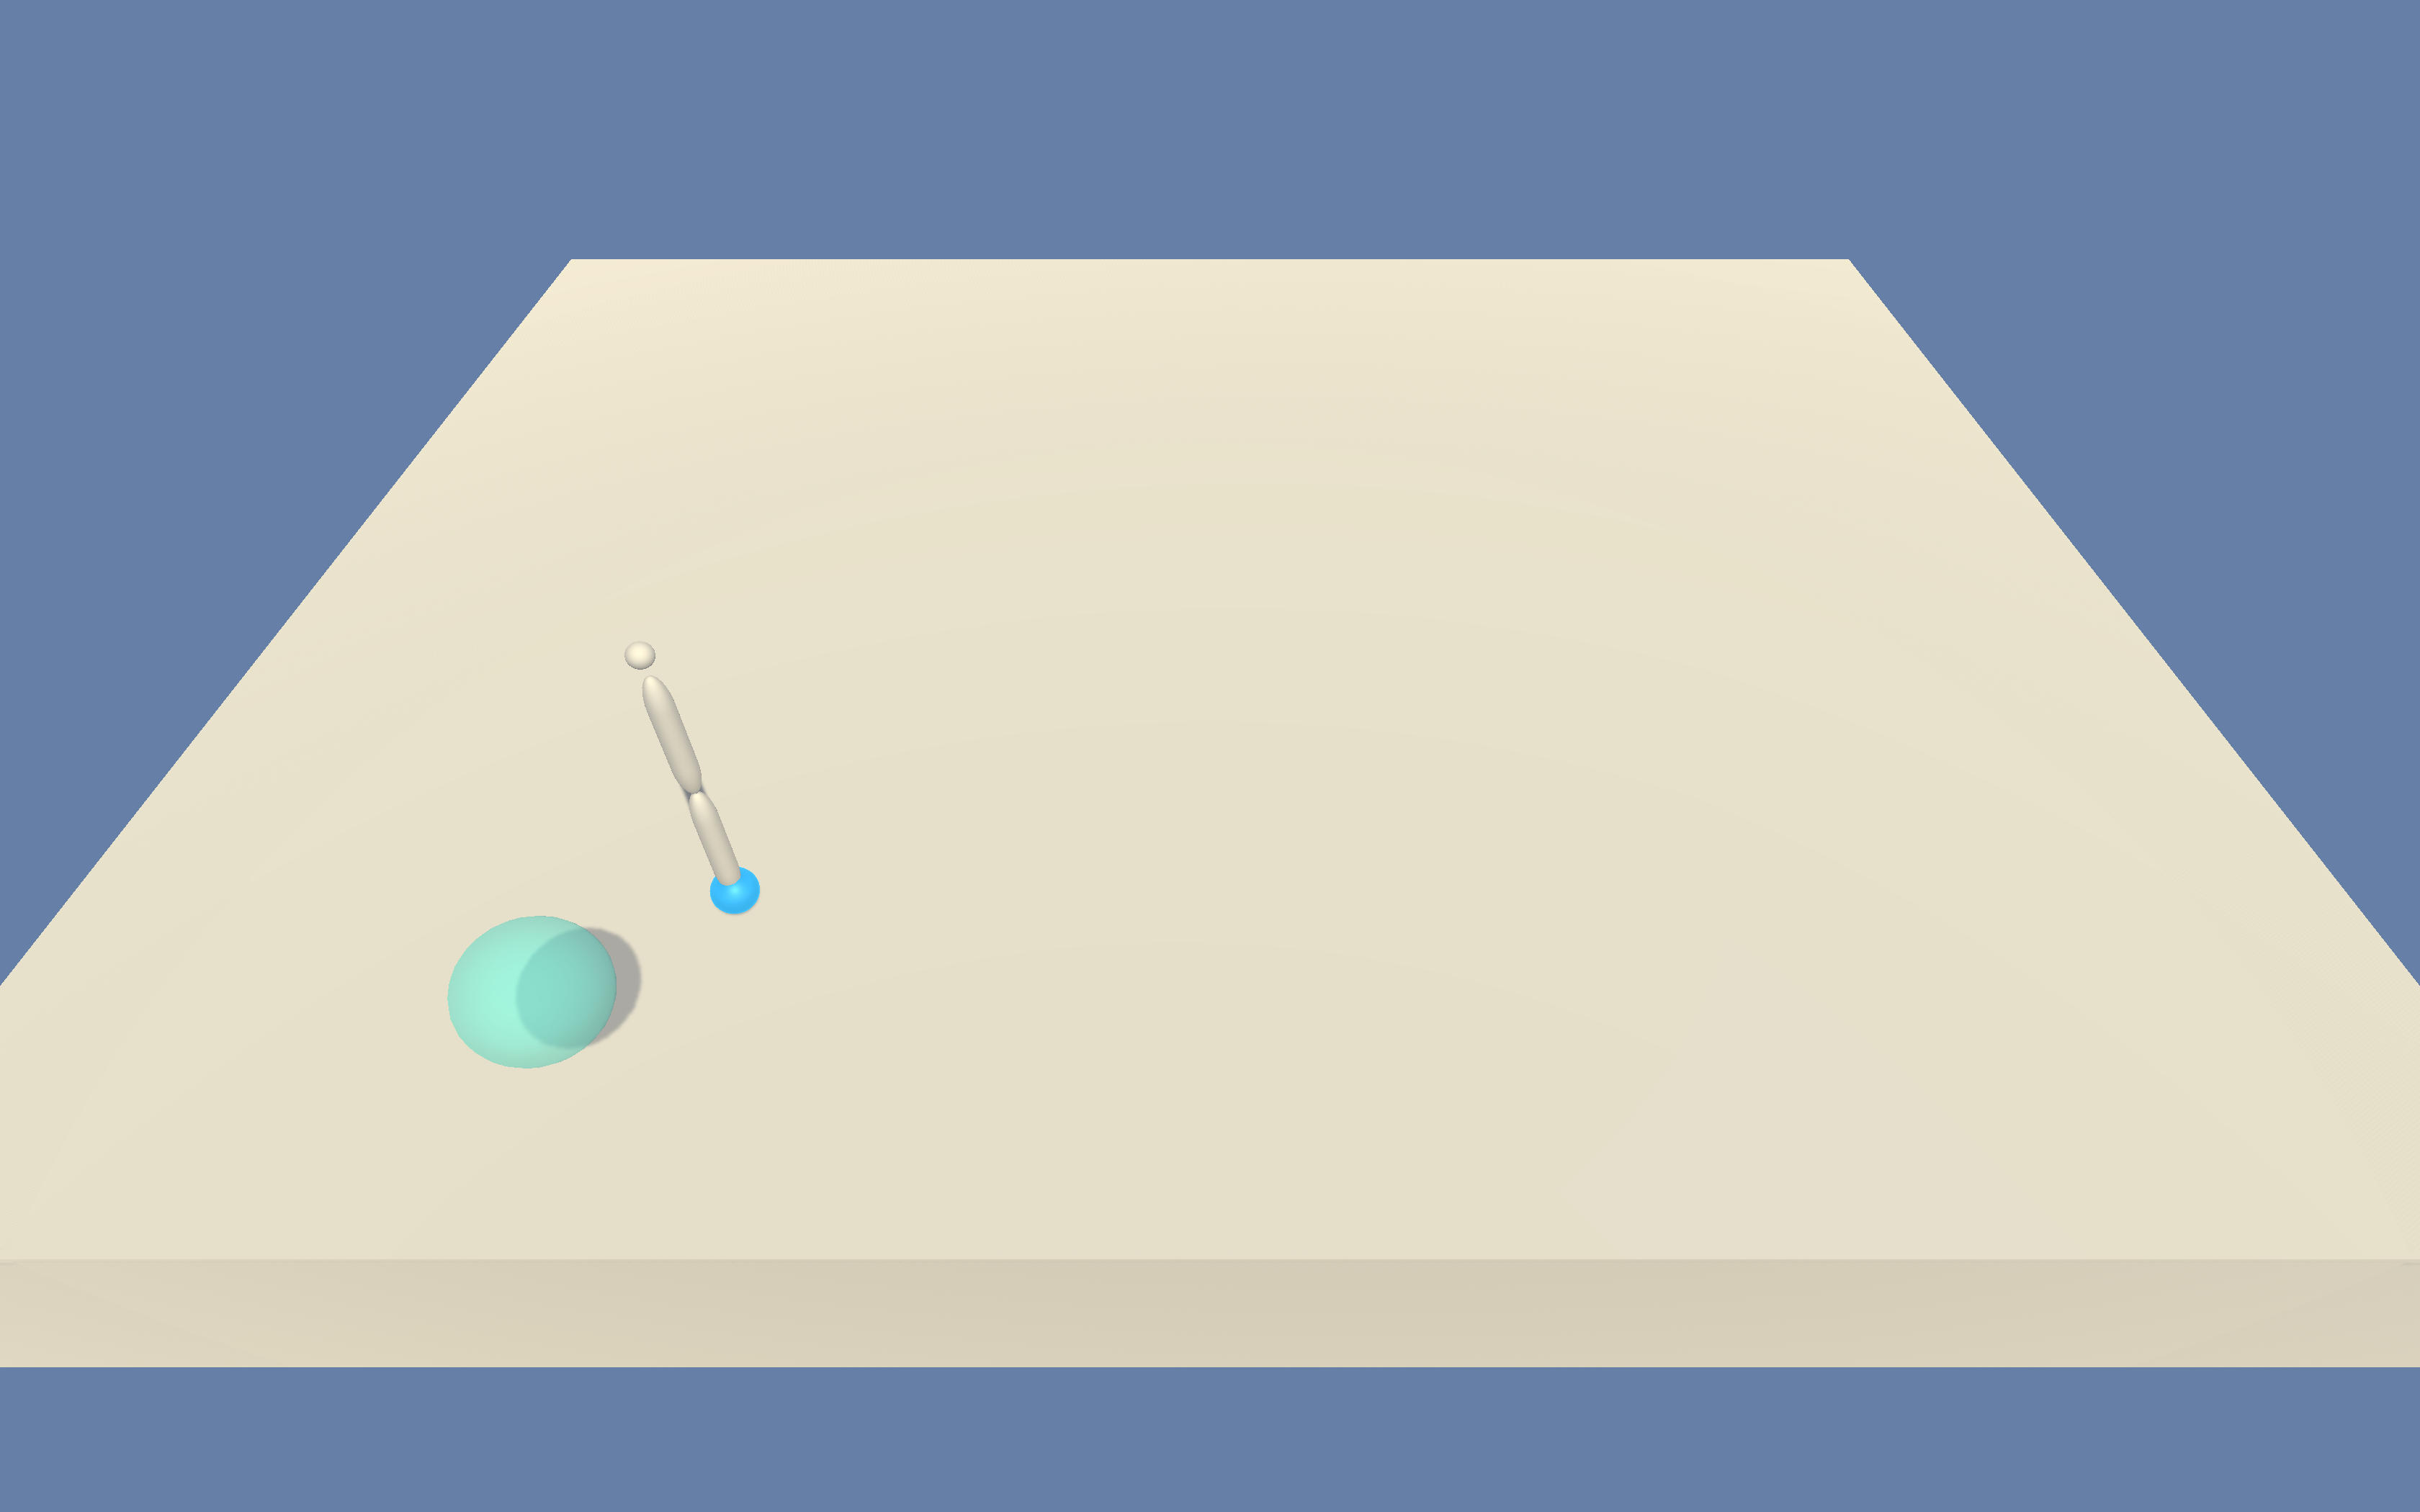
\includegraphics[width=0.7\linewidth]{figures/envs/unity_reacher_1.png}
            \caption{Unity Reacher Environment}
            \label{fig:unity_reacher_1}
    \end{center}
\end{figure}

\textbf{Multi-Agent Reacher:} in this environment, \textit{20 Agent} are used to parallelize the training process and collect more experiences and trajectories.

\begin{figure}[H]
    \begin{center}
            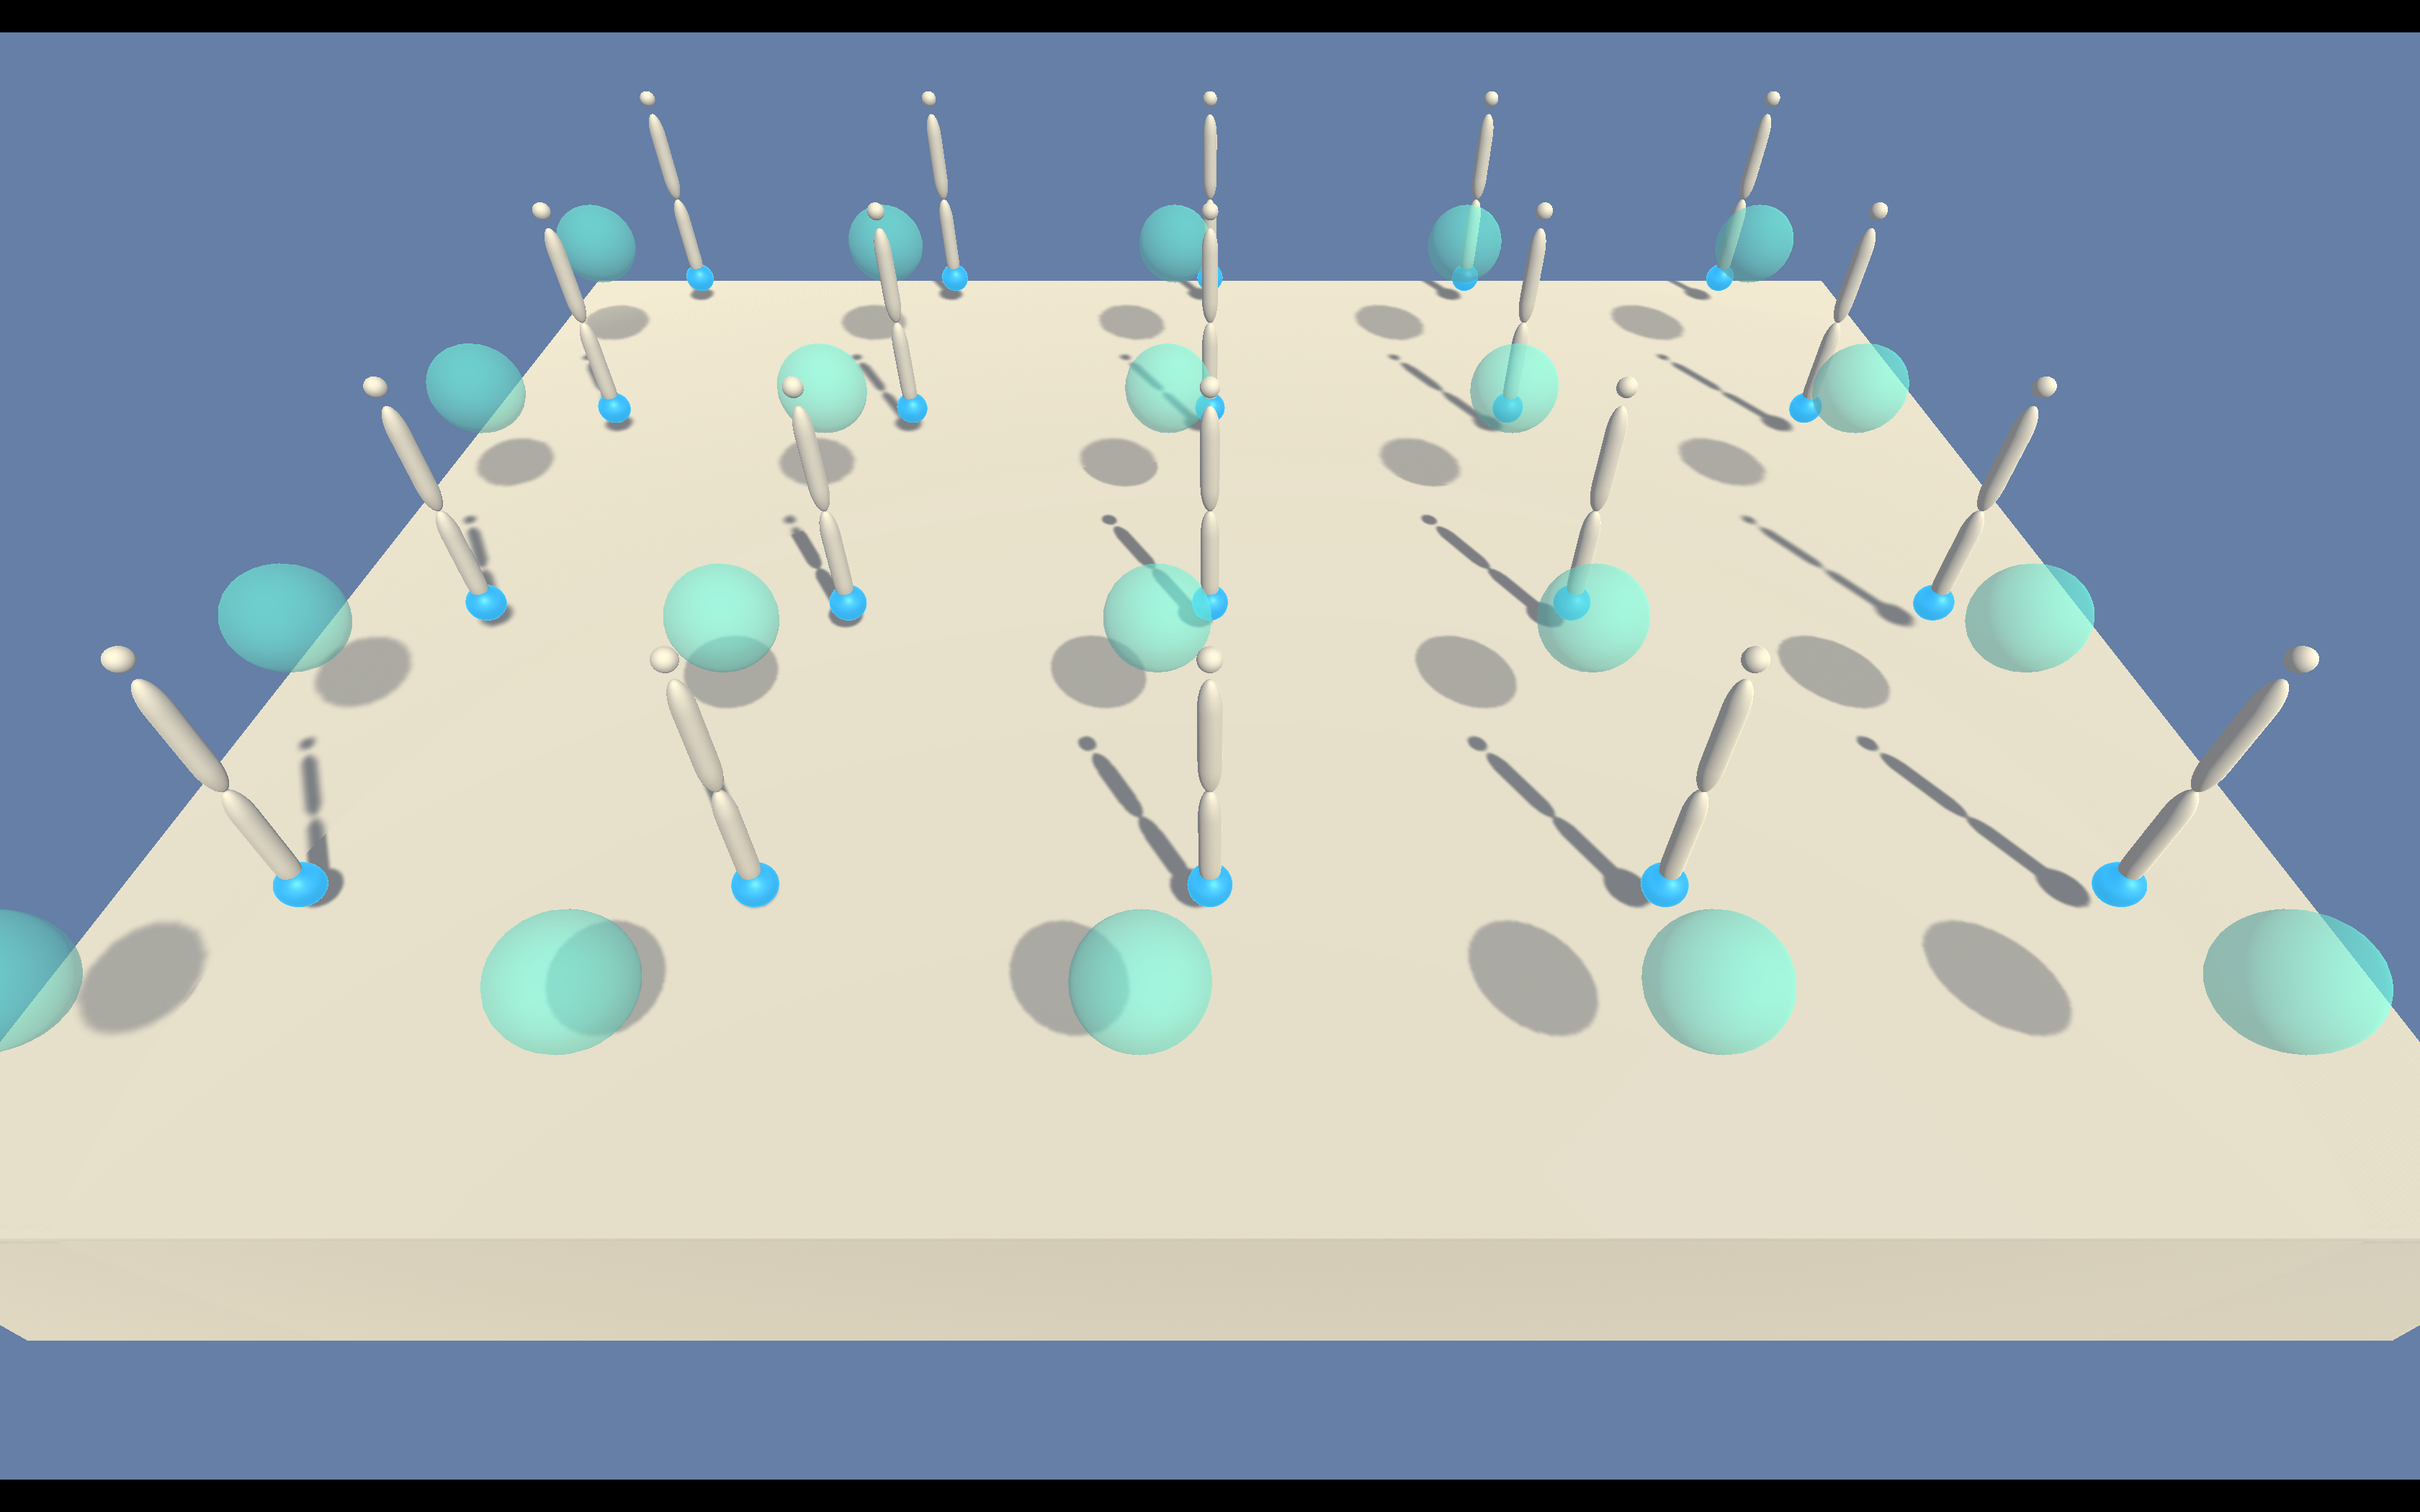
\includegraphics[width=0.7\linewidth]{figures/envs/unity_reacher_20.png}
            \caption{Unity Multi-Agent Reacher Environment}
            \label{fig:unity_reacher_20}
    \end{center}
\end{figure}



\chapter*{List of Abbreviations}
\addcontentsline{toc}{chapter}{List of Abbreviations}

\textbf{RL} - Reinforcement Learning

\noindent
\textbf{AGI} - Artificial General Intelligence

\noindent
\textbf{AI} - Artificial Intelligence

\noindent
\textbf{MCTS} - Monte-Carlo Tree Search 

\noindent
\textbf{TPU} - Tensor Processing Units

\noindent
\textbf{GPUs} - Graphical Processing Units 

\noindent
\textbf{CPU} - Central Processing Unit

\noindent
\textbf{MDP} - Markov Decision Processes

\noindent
\textbf{DRL} - Deep Reinforcement Learning

\noindent
\textbf{DQN} - Deep Q Network

\noindent
\textbf{DPG} - Deterministic Policy Gradient

\noindent
\textbf{DDPG} - Deep Deterministic Policy Gradient

\noindent
\textbf{PPO} - Proximal Policy Optimization

\noindent
\textbf{A2C} - Advanced Actor-Critic

\noindent
\textbf{A3C} - Asynchronous Advanced Actor Critic

\noindent
\textbf{NN} - Neural Network

\noindent
\textbf{SGD} - Stochastic Gradient Descent

\noindent
\textbf{Gorila} - General Reinforcement Learning Architecture

\noindent
\textbf{Ape-X} - Distributed Prioritized Experience Replay

\noindent
\textbf{IMPALA} - Importance Weighted Actor-Learner Architectures

\noindent
\textbf{} - 

\noindent
\textbf{} - 

\appendix{}

\chapter{Appendix}

If there are several additions you want to add, but they do not fit into the thesis itself, they belong here.

\section{Detailed Addition}

Even sections are possible, but usually only used for several elements in, e.g.\ tables, images, etc.

% \chapter{Figures}
% \section{Example 1}
% \cmark
% \section{Example 2}
% \xmark

\microtypesetup{protrusion=false}
\listoffigures{}
\listoftables{}
\microtypesetup{protrusion=true}
\printglossaries
\printbibliography{}

\end{document}
